% REV_P0 PREVIEW (2026-11-24): independent P0 scientific-text revision of the
% CellCharter research unit. V1 (…_v1_20261122) and layout V2 (…_layout_v2_20261123)
% remain unchanged. Typesetting settings are copied from layout V2; the appendix is
% the unchanged layout-V2 appendix (no E4 figure, caption or path changes).
% NOT compiled in the assistant session (no XeLaTeX on that machine).
% Not the user's full Master's dissertation; must be integrated into the school template.
\documentclass[UTF8,a4paper,12pt]{ctexart}
\usepackage[margin=2.4cm]{geometry}
\usepackage{amsmath,amssymb}
\usepackage{booktabs,tabularx,longtable}
\usepackage{graphicx,float}
\usepackage{caption}
\usepackage{url}
\usepackage[hidelinks]{hyperref}
\setlength{\parindent}{2em}
\setlength{\parskip}{0.08em}
\raggedbottom
\renewcommand{\arraystretch}{1.14}
\setcounter{secnumdepth}{3}
\begin{document}
% REV_P0 2026-11-24：由 cellcharter_study_introduction_module_v1_20261122.tex 派生；V1保持不变。
% 本轮只改写与CellCharter原作者已有DLPFC工作的重叠定位；证据见 REV_P0_20261124/REV_P0_EVIDENCE_TABLE_20261124.md。
% CellCharter研究专题引言模块（非整篇硕士毕业论文统一第一章）
% 可以根据导师确定的毕业论文总结构并入总论或专章绪论。
% 本文只覆盖第三篇空间聚类研究；不替代其他科研工作的引言。
\section{研究动机、目的与主要内容}
\label{sec:cc-intro-module-v1}

\subsection{研究动机}
随着空间转录组技术的发展，研究者能够把基因表达与组织采样位置联合分析，进而划分与分子特征和组织结构相关的空间域。然而，空间域划分的质量并不由算法名称单独决定。使用表达还是空间增强表示、引入多少层邻域信息、采用何种聚类数选择规则，以及用哪一类指标评价结果，都会影响聚类分析所得结论。

现有空间聚类框架已经提出多尺度邻域聚合、空间图表示学习与空间先验建模等机制。CellCharter作为其中一种成熟方法，可以在已有单点表示上叠加多层邻域信息\cite{varrone2024}。其原作者已在同一套12张DLPFC切片上完成基准比较：以151507、151672、151673三张切片调参，在其余9张切片上评价ARI；调参网格包括2、3、4层邻域，最终选用4层邻域、5000个高变基因和5维scVI潜变量\cite{varrone2024,cellcharteranalyses2024}。因此，“邻域层数会影响DLPFC聚类ARI”并非本研究的首次观察。但在实际数据分析中，扩大邻域表示范围与增加输入维数常常同时发生；若只比较单一数据集或少量随机初始化，容易将由聚类数、样本差异或标签粒度引起的变化误判成表示机制的必然优势。

空间转录组聚类还存在评价目标不同的问题。ARI和NMI比较预测分区与参考层标注的一致性，却不直接告诉研究者真实层间交界处是否发生边界错位或漏检。对于具有明确皮层分层的DLPFC和组织区域结构复杂的乳腺癌，这类差异在解释模型输出时尤其需要被单独记录。

\subsection{研究目的}
本研究不以提出一种新的空间聚类神经网络为目标，而是将已经公开的CellCharter表示与GMM聚类流程视为分析对象，通过一套尽量可复核的多条件评价，考察如下问题：在固定样本与聚类配置时，邻域深度和特征块组合的变化如何影响聚类分区；在不依赖参考类别数确定K时，上述观察是否稳定；整体ARI/NMI和严格空间边界指标是否提供一致的判断；结果与成熟基线相比处于什么水平，以及在另一组织患者队列上具有怎样的异质性。

由于这些问题涉及不同层级的实验比较，本研究分别定义Oracle-K与K-blind两类K设置，并保留原始预测、技术种子、参考mask及文件来源SHA。所有分析仅以已执行的实验为事实基础；对于研究完成后追加的诊断性评价，单独标注其为事后分析，不能将其当作前瞻性独立验证设计。

\subsection{研究内容}
为回答上述问题，本研究围绕12张DLPFC切片及6例乳腺癌Visium样本开展分阶段实验。

首先，基于已形成的scVI低维表达表示和CellCharter四层空间邻域聚合缓存，在DLPFC上比较5D至25D的累计特征与多种等维15D特征组合，并在10个技术种子上评价聚类结果。在5000个高变基因、5维潜变量条件下，累计15D、20D、25D分别对应原作者调参网格中的2、3、4层邻域，其中25D即原作者单切片基准的最终配置，可用于对照原作者已发表的结果；5D（不聚合）、10D（1层）和非连续的等维15D组合不在原作者网格中。其次，在同一冻结输入上设定固定K网格和无标签AutoK两类补充实验，分析聚类结果对簇数选择方式的敏感性。

再次，利用原有预测及六邻接阵列坐标，对严格空间边界的正确检出、误报和漏检进行重新审查，并分别提供1-hop、2-hop容差的事后敏感性评价。随后，在同一DLPFC切片上纳入非空间GMM、Leiden以及成熟空间方法BANKSY和BayesSpace，明确不同模型的原生数据处理及K选择差别。最后，在6名乳腺癌患者的独立数据上重新执行同类特征及基线流程，检查跨患者效果方向、低表现样本和方法间负结果。

\subsection{研究工作特点与论文组织}
本研究的主要特点是将多尺度特征、聚类数设置、边界评价、技术随机性与独立组织队列放在同一可追溯证据框架内；同时明确区分成熟方法与本文自行完成的实验分析，避免把已有邻域聚合操作写成新的算法结构。相对于原作者的DLPFC工作，本研究的新增内容限于以下几项：在全部12张切片、10个GMM种子上补充0层与1层累计特征以及非连续等维15D块替换（2--4层的比较与原作者调参网格重叠，仅样本范围和重复结构不同）；预设固定K网格；逐切片的无标签AutoK选K及其事后评分；ARI/NMI之外的严格与容差空间边界评价；双K策略下的成熟基线对照；以及乳腺癌6例患者的外部复核。上述内容均为实证评价，不构成新的聚类方法。具体结果并不以全部评价指标同向改善为前提，边界定位、不同患者的表现以及基线的局限都将作为真实结果完整呈现。

本专题的相关方法背景见后续研究背景部分，实际数据与技术路线见研究方法部分，完整结果和负面观察见实验结果与分析部分。上述内容可作为毕业论文中的一个独立研究专题，最终章节编号与其同其他论文工作的衔接由学位论文整体结构确定。

\clearpage
% REV_P0 2026-11-24：由 chapter_02_background_rewrite_v1_20261122.tex 派生；V1保持不变。
% 本轮已核对CellCharter原文正文、Methods、Fig.1、Extended Data Fig.1--2、10页Supplementary Information
% 及官方仓库CSOgroup/cellcharter_analyses（commit fd63ac5）；旧的“未核对补充材料”声明已改写。
% 第三篇CellCharter毕业论文第二章相关研究（2026-11-22）新版首稿
% 不覆盖历史chapter_02_background_integrated.tex；正文依赖主模板提供\cite。
% 参考文献条目在 thesis_cellcharter_verified_references_20261122.bib。
% 核查范围：已有项目11月11日文献证据矩阵 + 官网2026-11-22核对的BANKSY、BayesSpace、Leiden和Wu原文。
% 未逐项核对CellCharter的所有Supplement尺度消融，不能由“未报告”推断“没有前人做过”。
\section{研究背景与相关工作}
\label{sec:cc-background-rewrite-v1}

\subsection{空间转录组与组织空间域识别的研究需求}
\label{subsec:cc-st-background-v1}

基因表达谱为理解组织细胞状态、发育分化及疾病相关微环境提供了分子证据，但在不保留空间位置信息的测序设计中，细胞或组织区域间的原始相邻关系较难直接恢复。空间转录组测序通过将表达读数与组织中的采样坐标关联，使研究者能够同时考察表达相似性和空间结构。空间域识别（spatial domain identification）旨在将具有相近分子或空间特征的观测单位归入不同区域，所获得的聚类结果可用于探索组织分层、邻近细胞相互作用与肿瘤微环境等问题。

空间域聚类与一般表达聚类既有联系，也存在评价上的差别。对于表达聚类，两个来自相隔较远组织位置的spot可以因为表达相似而被分在同一个簇；对于空间域识别，同一簇在空间上是否连续、簇间交界能否对应真实组织结构，同样是具有解释价值的问题。反之，高度强调空间连续性也可能使小范围结构与清晰层间交界在模型输出中变得不易区分。因此，较高的总体聚类一致性并不自动意味着准确的空间边界定位，二者应有相互独立的评价证据。

人类背外侧前额叶皮层（dorsolateral prefrontal cortex，DLPFC）具有可观察的皮层分层结构，是空间域方法常用的真实数据场景。Maynard等发表了包含3位供体、12张Visium切片的DLPFC空间表达资料，并开展组织分层和表达结构研究\cite{maynard2021}。这些数据可用于检验模型是否能够恢复已有参考组织层，但应特别注意其采样结构：来自同一供体的不同切片并非彼此独立的生物学重复。此外，组织层的参考标注可能受到切片质量、标注来源和层间过渡区域的影响，不应把所有参考标签视为完美且无误差的绝对真值。

本研究除DLPFC外，还在另一种组织来源中评价方法流程。Wu等发布了人类乳腺癌的单细胞和空间分辨图谱，其公开数据中包含六例用于Visium空间分析的乳腺癌样本及相关空间元数据\cite{wu2021}。不同于皮层的层级结构，乳腺癌组织区域具有另一套病理标注语义，因此跨数据集比较的重点应是方法在新组织队列上的表现和患者异质性，而不是将DLPFC的ARI绝对值与乳腺癌的ARI绝对值直接比较后推断某一种组织更易分析。

\subsection{表达降维与空间信息的引入}
\label{subsec:cc-expression-v1}

空间表达矩阵通常维数较高，不同基因在测序深度、零计数比例和技术噪声方面存在差异。直接在全部基因上进行聚类，可能使计算成本和不稳定性同时增加。scVI（single-cell variational inference）是既有的概率深度生成建模框架，可从表达计数中学习适合下游分析的低维潜变量\cite{lopez2018}。本研究使用scVI作为已发表的表达表征工具，并将其5维潜变量作为单spot的基础特征，不涉及设计新的变分推断目标或神经网络结构。

只使用单spot表达，可能无法利用临近区域的组织上下文。空间聚类因而常将表达表示与组织坐标结合：一类方法首先通过表达构建低维表示，再从空间邻域聚合相邻点特征；另一类方法直接利用空间图或原生空间统计模型完成联合聚类。在具体实现上，不同方法可能使用空间最近邻、固定物理网格、像素坐标、阵列坐标或空间先验。它们所使用的空间结构虽然来源于同一组织，却并非一定是可互换的模型输入。因此，比较不同算法时应在统一样本和评价mask的前提下保留方法自身的输入定义，并避免宣称所有算法在完全相同特征与计算预算下受到控制。

SEDR（spatially embedded deep representation）等方法通过深度表示学习把空间联系纳入聚类过程。Xu等提出的SEDR框架包含掩码自监督表示学习与空间图表示等环节，说明“把空间信息引入表达表示”并不是单一模型的特有设计\cite{xu2024}。对本研究而言，其后续DLPFC参考标注的部分整理文件与SEDR相关公开分析资料有数据层面的联系，但标注文件存在于SEDR资料中不等于这些标签由SEDR模型生成，更不意味着标签由本研究重新人工标记。使用参考标签进行方法评价，应另行追溯其原始来源和加工过程。

\subsection{CellCharter及多尺度邻域表征}
\label{subsec:cc-cellcharter-v1}

CellCharter是由Varrone等提出的成熟空间生态位识别、表征及比较框架\cite{varrone2024}。其公开软件支持以已有表示为输入，对不同层数的空间邻域进行特征聚合，并将中心观测单位及多层邻域特征共同用于下游分析。官方软件接口提供聚合层数等参数，使研究者可以基于同一初始表达嵌入构建多尺度表示。本研究采用其公开实现及相应聚类功能，不将该邻域聚合算子本身表述为新提出的方法。

对于某一切片的$N$个spot，假设每个spot的scVI基础表示为5维，则可以把相应的CellCharter输出按顺序写为
\begin{equation}
H=[L_0\mid L_1\mid L_2\mid L_3\mid L_4]
\in\mathbb{R}^{N\times25},\quad L_\ell\in\mathbb{R}^{N\times5}.
\end{equation}
其中$L_0$对应原始基础表示，其余块与软件输出的不同邻域层相对应。在本项目中，该分块结构允许从同一25维冻结缓存中提取5D、10D、15D、20D、25D累计组合，也允许构造不同但维度相同的15D组合。后者适合检查“使用哪一层邻域块”是否与整体聚类和局部组织边界表现相关，但不能自动分离输入尺度、维数、空间拓扑和聚类数变化的全部效应。

多尺度空间信息的构建并非只有CellCharter一种途径。例如，m2ST的研究已讨论多尺度图表示及尺度信息的融合问题\cite{zhang2025}。已有工作还将不同尺度的贡献作为可调对象，说明仅提出“更深邻域可能有用”或者“按不同尺度拼接特征”，不足以建立新的核心算法贡献。本研究因此采用实证评价的定位：明确固定不同维度、等维替换、K选择规则和评价指标，关注在真实数据中哪些结论相对稳定、哪些条件会出现方向相反的结果。

\subsubsection{原作者在DLPFC上已完成的工作}
\label{subsubsec:cc-prior-dlpfc-rev-p0}
CellCharter原文已使用本研究所用的同一套12张DLPFC Visium切片进行基准比较\cite{varrone2024}，与本研究直接相关的内容如下：
\begin{enumerate}
  \item \textbf{调参与测试划分。}原文Methods中“Benchmarking comparison of CellCharter with existing tools”一节规定：每位供体随机选1张切片（151507、151672、151673）组成调参集，用网格搜索、每组参数5次重复、取调参集平均ARI最大者确定超参数；其余9张切片作为测试集，每张重复10次，仅以ARI评价，未标注spot参与聚类、不参与评分。Extended Data Fig.~1e、1f对比了“在同一数据上调参和测试”与“调参集与测试集分离”两种做法。
  \item \textbf{邻域层数已被调参。}Supplementary Information“Hyperparameter tuning: grid search”一节列出CellCharter的候选值：高变基因$\{500,1000,2000,5000\}$，选5000；潜变量维度$\{5,10,15\}$，选5；邻域层数$\{2,3,4\}$，选4。官方仓库\texttt{src/benchmarking/CellCharter/tuning.py}与\texttt{ARI\_CellCharter\_tuning.csv}给出这一网格的逐格ARI\cite{cellcharteranalyses2024}。因此在5000高变基因、5维潜变量条件下，2--4层邻域对ARI的影响已有原作者在3张调参切片上的评价。
  \item \textbf{单切片与联合聚类。}原作者统一要求各方法输出7个簇（Results正文）；但官方单切片脚本\texttt{individual.py}对151669--151672设$K=5$、其余设$K=7$，与本研究的Oracle-K相同。原文的主要性能结论来自9张测试切片的\textbf{联合聚类}（Fig.~1d、1e；Extended Data Fig.~1h）。在\textbf{单切片}聚类中，原文报告STAGATE表现最好（Extended Data Fig.~1g）\cite{dong2022stagate}。
  \item \textbf{无标签选K。}CellCharter的选K规则是：对每个候选K重复拟合GMM，按K、$K-1$、$K+1$的Fowlkes--Mallows指数\cite{fowlkes1983}判断稳定性（原文Fig.~1a及Methods“Cluster stability”）。在DLPFC上，原作者对全部12张切片\textbf{联合}运行该规则（候选2--20，10次重复），稳定性峰值为$n=9$。同一设置下BIC的全局最小值在$n=19$，AIC与负对数似然没有清晰拐点（Fig.~1h；Extended Data Fig.~2b；Supplementary Information中关于cluster stability与AIC/BIC/NLL比较的一节）。
\end{enumerate}

据此，本研究与原作者工作的重叠和差异如下。重叠部分包括：25D配置、Oracle-K设置、ARI评价，以及2--4层邻域对ARI影响的比较方向。本研究另外完成的部分包括：0层与1层累计特征和非连续等维15D组合；在全部12张切片上每切片10个GMM种子的重复结构；预设固定K网格（E3c）；\textbf{逐切片}的稳定性AutoK及其事后ARI/NMI；严格与容差空间边界指标；BANKSY与BayesSpace双K臂对照；乳腺癌外部队列。原作者的无标签选K是在联合样本上作示例，而不是逐切片的标签评分。本研究不作“首次发现聚合尺度影响聚类性能”的声明；对于“既有研究未评估空间边界”，本研究只核对了CellCharter原文与官方仓库，不能推广到全部文献。

\subsection{成熟聚类基线与不同K选择方式}
\label{subsec:cc-baselines-background-v1}

非空间GMM是常见的概率混合聚类思路，能够将低维表达表示划分成若干统计成分；但在本项目的非空间基线中，其输入不包含显式组织坐标。以BIC等似然准则为GMM选K时，结果容易偏向更多簇；CellCharter原作者在DLPFC联合数据上也观察到BIC建议的簇数（$n=19$）明显多于稳定性峰值（$n=9$）\cite{varrone2024}。Leiden是一种图社区发现算法，Traag等针对图社区划分提出了保证社区连通性的改进方法\cite{traag2019}。当Leiden用于表达近邻图时，其邻居关系主要由表达表征建立，并不自动等于组织中的物理空间六邻接。二者作为非空间对照，有助于描述额外引入空间表示后可能出现的评价差异。

BANKSY通过融合自身表达及邻域信息构建空间增强的表示，并可结合下游聚类完成空间域识别；其原始研究还展示了组织域分割和细胞类型分析等任务\cite{singhal2024}。BayesSpace则采用低维表达与空间先验相结合的统计模型进行空间聚类，并可支持更精细的空间区域推断\cite{zhao2021}。这两种方法依赖不同的原生空间表示和参数选择程序，不能因为都引入了空间信息就认定它们的计算量或聚类数选择机制等价。

除了模型本身，预测簇数$K$的确定方式也会显著影响结果解释。若直接以人工参考标签的类别数量设置$K$，这实际上使用了标签类别数先验，本文称之为\textit{Oracle-K}。即使模型拟合过程没有读入每个spot的参考层标签，该类别数量仍会影响最终输出。相对地，\textit{K-blind}表示在决定K或无监督分辨率时不使用人工参考层类别信息，例如依据稳定性或BIC的预设规则，或采用固定分辨率。两者应分表呈现，不能把Oracle-K的表现误写成完全无标签的真实部署能力。

不同原生方法也存在选K判据的适用条件。以BayesSpace为例，其\texttt{qTune}给出不同候选q的平均伪对数似然，官方使用说明建议\textbf{在\texttt{qPlot}曲线的拐点（elbow）附近选q}\cite{bayesspacevignette}。本研究冻结的K-blind规则是取平均伪对数似然最大的q，\textbf{与官方建议不一致}；该规则在本研究数据上频繁选中搜索上界（见第\ref{subsec:cellcharter-e5a-v1}节）。原冻结结果全部保留，不在观察结果后更换判据。这一问题属于对照协议的系统性缺陷，会降低BayesSpace在K-blind条件下的可比性，不能当作随机波动处理。

\subsection{聚类指标、空间边界与参考标注的评价问题}
\label{subsec:cc-evaluation-background-v1}

ARI（adjusted Rand index）和NMI（normalized mutual information）是比较预测聚类与参考标签的一类常用指标，二者均不依赖预测簇名称本身的编号。ARI具有机会校正的随机划分参照，NMI衡量两种分区之间的共享信息，但两者本质上比较的是观测单位所属的类别划分，而不是直接测量组织空间边界定位。如果一个算法把相邻真实层间交界略微移开，即使总体ARI没有明显变化，该偏移仍可能改变组织学边界检出的结果；反过来，较少的预测边界也可能同时减少误报和漏检，综合F1需要结合基础计数理解。

基于此，本研究在Visium阵列六邻接图上设置严格edge-F1，以相邻两个spot的参考层是否不同作为真实边界、预测簇是否不同作为预测边界；同时记录TP、FP、FN以区分正确检出、误报和漏检。考虑到严格网格边匹配对少量位置偏移敏感，另将1-hop和2-hop容差作为明确标注的\textbf{事后敏感性分析}，在有效边的线图中使用一对一匹配，避免同一参考边界被重复计算。宽松容差可以回答“邻近交界是否被预测”，不能代替严格定位结果，更不能根据哪个容差指标更有利再调整主评价目标。

已有针对空间聚类评价的研究也提示，在数据处理、标签质量和模型调节条件不同的情况下，性能排序具有不确定性。例如，SACCELERATOR围绕空间感知聚类的评价与专家参与参考机制提出了相关讨论\cite{sun2026}。本研究不将全部参考标签等同于绝对无误差的生物学真值；对于DLPFC皮层层级和乳腺癌病理区域，必须分别说明其标签粒度、数据来源、有效mask和不可直接互换的语义。

对于DLPFC，12张切片来源于3位供体，同一供体内的空间邻近切片不是12份独立受试者；对于外部队列，则有6名不同患者。技术随机种子只能描述算法初始化或拟合波动，不能增加生物学样本量。因此，本研究优先报告按切片/患者分层的效应量、方向一致性、负结果及解释限制，不以spot、边或seed数目制造显著性。该处理也是将整体ARI/NMI与局部边界评价放在同一证据框架中的必要前提。

\subsection{研究问题与本文工作定位}
\label{subsec:cc-questions-background-v1}

结合以上方法特征与评价限制，本研究使用成熟CellCharter流程形成可复核的系统实证评价，具体围绕如下研究问题：
\begin{enumerate}
  \item 在固定数据、GMM与Oracle-K条件下，累计邻域深度和等维邻域块替换如何影响DLPFC整体聚类指标？这一影响对技术随机种子和切片/供体是否稳定？
  \item 当K通过固定网格或不读取人工标签的AutoK规则决定时，尺度比较结果是否发生变化？选K边界和不同实际簇数应如何呈现？
  \item 严格空间边界F1与1-hop、2-hop邻近容差F1是否给出相同尺度排序？误报与漏检是否存在解释上的权衡？
  \item 在同一DLPFC数据上与非空间及成熟空间方法比较时，K-blind/Oracle-K和原生预处理差异会如何限制结论？
  \item 将同类流程重新用于六名乳腺癌患者时，邻域尺度的描述性收益是否具有患者间的一致性；哪些失败与负结果不能被宏平均遮盖？
\end{enumerate}

本文不把这些问题包装成新基础算法的提出和性能保证。研究工作包括真实DLPFC数据的多尺度与选K实验、冻结预测的空间边界和容差评价、成熟基线的双K策略对照、独立外部患者队列的重复分析，以及对所有原始预测、来源SHA和评价脚本的归档。现有实验证据支持的是在所选样本与协议下对方法行为的描述和评价；是否对其他组织、平台或更大患者群体成立，仍需要额外证据，而不能由本章直接推断。

\clearpage
% REV_P0 2026-11-24：由 chapter_03_methods_rewrite_v1_20261122.tex 派生；V1保持不变。
% 新增：与原作者DLPFC基准的预处理/K/重复结构逐项对照；B15D提名经过；AutoK重复次数差异；
% BayesSpace与GMM K-blind规则缺陷；技术seed SD的含义。未改动任何冻结协议参数或实验数据。
% 第三篇CellCharter毕业论文第三章（2026-11-22）新版首稿
% 研究对象：DLPFC 12切片 + Wu等外部6患者，不涉及本账号其他论文。
% 保留 chapter_03_methods_integrated.tex 历史原稿；本稿不覆盖旧稿。
% 本文件是待嵌入学校主LaTeX模板的正文片段；依赖 booktabs、amsmath 等宏包。
% 真实结果数值见 chapter_04_results_rewrite_v1_20261122.tex 和来源审查矩阵。
% E3d后验ARI/NMI与E3b容差是模型已完成、研究者已看过其他结果后进行的事后分析。
\section{研究方法与实验方案}
\label{sec:cellcharter-methods-v1}

\subsection{研究思路与技术路线}
\label{subsec:cc-overview-v1}

空间转录组测序技术可以在组织位置上同时获得基因表达信息，为空间域（spatial domain）识别提供了数据基础。空间聚类既受到原始表达特征的影响，也受到邻接结构、聚类数选择和组织标注粒度的影响。因此，仅报告单一算法在某张切片上的最高ARI不足以反映实际结果的稳定性。本研究以成熟的CellCharter邻域聚合与聚类实现为基础，重点分析不同尺度表示、聚类数确定方式和评价定义对空间域聚类结论的影响；同时设置非空间及空间成熟方法作为对照，并使用不同组织来源的数据进行独立队列评估。

研究程序分为六个相互衔接但证据性质不同的阶段：（1）在12张DLPFC切片上构建并审计5维scVI潜在表示及25维CellCharter多尺度缓存；（2）固定Oracle-K与10技术种子比较10种邻域特征组织方式（E1/E2）；（3）以预定K网格检查尺度结论对簇数的敏感性（E3c），再以无标签AutoK实现独立选择K（E3d）；（4）从已保存的预测与原始六邻接阵列坐标重新计算严格空间边界和容差指标（E3b）；（5）在相同DLPFC切片上对照四种成熟基线（E5a）；（6）在6名乳腺癌患者的独立来源数据上重新执行同类方法，报告跨组织实验流程的表现（E5b）。E4空间图及标记基因表达图用于辅助解释，不参与前述特征或K参数的选择。

以上各阶段不是将一个在DLPFC训练完成的聚类模型迁移至乳腺癌，也不构成对CellCharter底层邻域聚合公式的原创改造。各阶段的原始冻结协议、预测及指标文件、计算脚本和审计记录均以项目实际归档版本为准。对实验结束后才新增的诊断性评价，本文在方法和结果中单独说明为事后分析，不将其倒写为早期已预注册的主研究终点。

\subsection{数据来源、样本层级与参考标注}
\label{subsec:cc-data-v1}

\subsubsection{DLPFC人脑组织切片}
DLPFC评价集由12张Visium空间转录组切片组成，切片标识依次为151507、151508、151509、151510、151669、151670、151671、151672、151673、151674、151675、151676。样本按来源分为3位供体，每位供体4张切片。既有归档供体映射中，151507--151510对应一组，151669--151672对应一组，151673--151676对应另一组；部分早期切片的供体对应关系依据公开附录佐证而非本研究重新取得并验证的全部原始受试者元数据，因此在最终统计解释中保留该证据限制。

每张切片采用原始10x \texttt{filtered\_feature\_bc\_matrix.h5}表达计数文件，空间位置信息来自\texttt{spots\_aligned.csv}，其中的barcode、\texttt{array\_row}、\texttt{array\_col}及像素坐标与源数据按唯一barcode匹配。人工参考组织层标签从\texttt{manual\_layer\_annotations.csv}读取，并根据\texttt{sample\_name}与\texttt{spot\_name}进行对齐。标注缺失的spot可保留于模型输入与空间可视化，但不纳入ARI、NMI或有效参考边界的计分。不得把未经重新病理判读的公开参考标签表述为本研究新制作的组织学金标准。

151507、151508的早期开发性参考文件与后续10片的标准化标签来源路径不完全相同。后续10张切片涉及已有\texttt{layer\_guess}及其顺序调整字段的核对；本研究按冻结的标准化标签与评价mask复用，不因结果重新修改。曾发现151507目录中存在与151669重复的错误\texttt{metadata.tsv}副本，按原数据审计记录该文件不被当前E1/E2聚类评价任务直接读取；这不等于证明所有更早的特征缓存生成过程完全不受任何数据卫生风险影响。上述问题作为来源质量与解释限制保留，不以人工修补方式改变本次已冻结预测。

\subsubsection{乳腺癌独立队列}
外部评价采用Wu等研究公开的6例人乳腺癌Visium数据，患者标识为1142243F、1160920F、CID4290、CID4465、CID44971及CID4535。源数据包含表达计数、空间坐标和供评价使用的组织区域标签；原始来源及压缩文件的MD5哈希已在实验前核对，患者标识互不相同。本研究的外部数据意在检验同类无监督聚类流程与邻域深度比较在另一组织来源下的表现，而非验证皮层空间域模型的直接跨器官预测能力，也不是医学诊断性能验证。

根据冻结输入审计记录，6名患者分别具有4784、4895、2426、1211、1160和1125个用于模型计算的spot；对应评价mask包含4665、4846、2419、1207、1159和1028个spot，合计15601个模型spot和15324个评价spot。评价spot数量不等于生物学重复次数。本文以6名不同患者作为独立生物学单位，spot、技术seed、尺度条件和预测任务均为患者内观察。

\subsubsection{样本独立性与数据使用边界}
DLPFC的独立生物学层级为供体$n=3$，每供体4张切片；外部数据的独立生物学层级为患者$n=6$。在计算时可以报告每切片或每患者的单独分数及其技术重复间变异，但不以同一供体的4张切片、同一患者的多个spot或同一实验条件的多个随机种子扩增统计检验样本量。DLPFC包含开发性探索过程，不将其12张切片全部描述为严格未接触的测试样本；外部队列在原方案冻结之后进行，但后续事后统计摘要仍须如实披露时间线。

\subsection{表达预处理与scVI特征缓存}
\label{subsec:cc-preprocess-v1}
DLPFC采用现有已审计的源处理和特征生成结果，按唯一barcode对齐空间位置表及表达矩阵。此前准备脚本将基因名规范为唯一，按计数阈值进行过滤并验证spot/barcode约束；在\texttt{counts}层保留原始计数，进行总量归一化与对数转换，并以基于原计数的\texttt{seurat\_v3}方法选择5000个高变基因。scVI通过\texttt{scvi.model.SCVI.setup\_anndata(..., layer="counts")}读取计数层，生成潜变量维度为5的表示。此处scVI拟合输入为计数层，而不是误将已归一化对数矩阵称为直接的原始计数输入。

DLPFC来源训练脚本的主要设置包括随机种子22911、最大400训练轮次和early stopping；新增10张切片源流程曾要求CUDA环境。训练轮次上限不意味着每张切片都运行满400轮。每张切片形成的低维潜变量矩阵记为
\begin{equation}
Z=[z_1^\top,\ldots,z_N^\top]^\top\in\mathbb{R}^{N\times5},
\end{equation}
其中$N$为相应切片纳入建模的spot数。既有5维与25维特征缓存均伴随spot顺序、源哈希和生成记录保存；后续E1/E2、E3c、E3d从同一冻结特征缓存抽取所需列，不因评价数值重新训练scVI。

上述DLPFC特征流程（\texttt{scripts/cellcharter/prepare\_dlpfc\_10\_features.py}）与CellCharter官方单切片基准脚本\texttt{src/benchmarking/CellCharter/individual.py}\cite{cellcharteranalyses2024}的主要步骤相同，包括：\texttt{filter\_genes}与\texttt{filter\_cells}的\texttt{min\_counts=3}、总量归一化至$10^6$并取对数、在计数层上以\texttt{seurat\_v3}选5000个高变基因、5维scVI潜变量、AdamW优化器配合early stopping与\texttt{reduce\_lr\_on\_plateau}、4层邻域聚合。表\ref{tab:cc-official-protocol-rev-p0}逐项列出两者已知的差异。由于存在这些差异，即使两者数值相近，也不能视为逐spot等价的复现。

\begin{table}[htbp]
\centering
\caption{本研究DLPFC 25D流程与CellCharter官方单切片基准的设置对照（依据双方脚本；未核对的项目注明“未核对”）}
\label{tab:cc-official-protocol-rev-p0}
\small
\begin{tabularx}{\linewidth}{p{2.6cm}XX}
\toprule
项目 & 官方单切片基准\cite{cellcharteranalyses2024} & 本研究E1/E2\\
\midrule
切片范围 & 12张均运行；原文图件只报告9张测试切片 & 12张\\
聚类方式 & 单切片（\texttt{individual.py}）；原文主结论为9切片联合聚类 & 单切片\\
K & 151669--151672为5，其余为7 & 同左（Oracle-K）\\
重复结构 & 10次，每次同时更换scVI与GMM的种子 & scVI固定种子22911训练一次；10个GMM种子\\
scVI轮次 & 默认上限，early stopping & 上限400，early stopping\\
GMM设置 & \texttt{cc.tl.SpatialCluster}默认参数，GPU & CellCharter GMM接口，CPU，容差$10^{-3}$，正则$10^{-6}$，最多100 epoch\\
输入文件 & HumanPilot预处理h5ad & 10x \texttt{filtered\_feature\_bc\_matrix.h5}与\texttt{spots\_aligned.csv}\\
参考标签字段 & \texttt{sce.layer\_guess} & \texttt{layer\_guess}经\texttt{manual\_layer\_annotations.csv}对齐\\
软件版本 & 未核对 & 记录于各缓存\texttt{config.json}\\
评价指标 & 仅ARI & ARI、NMI，另有事后边界指标\\
\bottomrule
\end{tabularx}
\end{table}

乳腺癌队列则在每名患者各自的计数数据上重新完成标准化输入与scVI五维表征，再建立患者内CellCharter空间邻域聚合特征。外部批次的模型训练、计算设备和输出状态以\texttt{e5b\_scvi\_feature\_batch\_v1.py}及相应Windows审计为准。该过程并未加载DLPFC训练的scVI权重做跨组织迁移；因此跨数据集比较评价的是流程的重复应用，而非既训练模型的domain generalization。

\subsection{空间六邻接图与CellCharter多尺度表示}
\label{subsec:cc-spatial-v1}

使用Visium阵列中spot的\texttt{array\_row}、\texttt{array\_col}建立空间邻接图$G=(V,E)$，其中每个节点对应一个spot。对有效直接邻居，阵列偏移满足
\begin{equation}
(|\Delta r|,|\Delta c|)\in\{(0,2),(1,1)\}.
\label{eq:cc-hex-v1}
\end{equation}
上述条件对应六角阵列的六种最近邻方向；边按无向关系记录，排除自环、重复坐标和不匹配barcode。该图按空间物理布局建立，不以表达量距离定义基因表达kNN图。不同方法如BANKSY和BayesSpace会按照各自原生实现使用空间坐标，其空间邻居定义不应与本节CellCharter的六邻接边混为同一算法。

本研究沿用CellCharter官方实现的\texttt{aggregate\_neighbors}操作，以5维scVI表征为输入，聚合4层并将原始层与聚合层拼接成
\begin{equation}
H=[L_0\mid L_1\mid L_2\mid L_3\mid L_4]
\in\mathbb{R}^{N\times25},\qquad
L_\ell\in\mathbb{R}^{N\times5}.
\label{eq:cc-H-v1}
\end{equation}
$L_0$为未聚合的5维输入层，$L_1$--$L_4$为CellCharter程序输出的相应邻域块。这里的层级是软件特征块索引，不将某一层直接赋予已验证的组织学影响半径；也不臆造CellCharter内部未逐项核实的加权公式。缓存中的列顺序、spot对齐和SHA由前期脚本及审计记录锁定。

固定的累计邻域特征为$L_0$（5D）、$[L_0,L_1]$（10D）、$[L_0,L_1,L_2]$（15D）、$[L_0,\ldots,L_3]$（20D）、$[L_0,\ldots,L_4]$（25D）。另设5种等维但不连续的15D组合，分别为$[L_0,L_1,L_3]$、$[L_0,L_1,L_4]$、$[L_0,L_2,L_3]$、$[L_0,L_2,L_4]$和$[L_0,L_3,L_4]$。其中标准15D配置A为$[L_0,L_1,L_2]$，候选B为$[L_0,L_1,L_4]$。A/B保持输入维度一致，但不代表其他未控制的模型差异全部消失；候选B亦不构成新的CellCharter核心模型。

需要说明两点数据使用情况。其一，4层邻域、5000高变基因、5维潜变量这组参数，是CellCharter原作者在151507、151672、151673上按参考标签ARI调出的\cite{varrone2024}；本研究直接沿用，因此这3张切片对25D配置不是未接触样本。其二，候选B是在开发切片151507（Oracle-K=7，GMM种子22911）上看到B相对A的ARI高出0.047后才被提名的；151507与151508都属于开发阶段已分析过的切片，随后又和其余10张切片一起纳入E1/E2完整评价。因此，E1/E2中B与A的比较带有提名切片的选择偏倚。结果部分同时报告预设的12切片汇总和排除这两张开发切片后的事后敏感性汇总，两者分别解释。

\subsection{DLPFC冻结聚类实验设计}
\label{subsec:cc-dlpfc-protocol-v1}

\subsubsection{E1/E2：十种特征配置与十技术种子}
E1/E2固定12张DLPFC切片、10种特征配置和10个随机种子，共形成$12\times10\times10=1200$个切片--配置--seed评价任务。预定种子序列为22911、7449、25842、10379、6690、26128、21059、22159、32389和12815。所有条件使用CellCharter的GMM聚类接口（CPU、full covariance、K-means初始化、收敛容差$10^{-3}$、协方差正则$10^{-6}$、最多100 epoch），统一记录拟合结果、实际簇数、评价mask和源文件哈希。为避免重计历史运行，若个别已存任务与冻结配置和文件SHA完全一致，则审计合格后复用；1200指完整任务网格而非全部1200项均在同一批次重新计算。

此阶段使用参考标签类别数确定K：151669--151672的4张切片设$K=5$，其余8张设$K=7$。这是明确的\textit{Oracle-K}条件。单个spot的层标注不用于GMM参数估计，但使用参考类别数本身已经带入了标签先验，不能称其为完全不依赖参考标签的聚类数选择。各模型先落盘预测及其SHA后再以固定标签mask进行指标评价，不依据ARI/NMI回选最有利种子。

\subsubsection{E3c：固定K敏感性网格}
E3c进一步在12张切片、4种累计尺度（10/15/20/25D）、5个指定K（5至9）和前述10种子上建立$12\times4\times5\times10=2400$格敏感性网格。其中480格与已通过审计的E1/E2 Oracle-K条件重合，予以复用；其余1920格为新形成的评价结果。固定K网格是对预设聚类数的受控比较，不意味着算法已自动估计未知K；报告每张切片、每个K和每个尺度的全部ARI、NMI及负结果，而不依据参考标签选择最终推荐K。E3c与E1/E2使用相同冻结特征缓存和对应GMM配置。

\subsubsection{E3d：无标签AutoK稳定性选K}
E3d独立使用12切片和四个累计尺度，构成48个K-blind AutoK配置。冻结候选集合为$K\in\{2,3,\ldots,10\}$，CellCharter实现中同时拟合辅助K=1与11；每个内部K进行5次GMM初始化，正式使用CPU、满5次稳定性尝试与明确seed22911--22915。按稳定性均值最大确定K，并保留原程序的首个最大值并列处理。每组合内部记录$11\times5=55$次模型拟合标签档案，全部48组合对应2640份内部运行标签阵列。该过程使用固定输入及无标签稳定性，人工组织层标签不进入拟合、早停或K选择。

E3d与原作者的稳定性选K示例有两点不同。第一，本研究每个候选K只重复5次，原作者在DLPFC上使用10次（原文Fig.~1a说明与Methods）；原作者还在Supplementary Information中把重复次数增加到25次，检查10次是否已使FMI曲线收敛。本研究的5次重复未做这一收敛检查，因此不能排除重复次数不足造成的选K不稳定。第二，原作者是对12张切片\textbf{联合}运行选K，本研究是对每张切片\textbf{单独}运行。E3d的结果应理解为“5次重复、逐切片”条件下的表现，不等同于原作者推荐设置下的表现。

AutoK输出在完成之后冻结：保存每个切片--尺度的原选中K、各候选K的稳定性、唯一barcode对应的聚类预测、版本与来源SHA；先进行不看参考标签的独立文件审计。直到48项原始预测全部审计通过，才单独使用固定参考标签mask对其计算ARI/NMI。这一指标计算是在观察过其他实验结果后追加的\textbf{事后后验评价}；不能倒称E3d原冻结训练阶段已经完成标签评分。对于选中K=2或10的边界情形，如实记录而不事后扩K或重新拟合。

\subsection{空间边界与拓扑容差的事后评价（E3b）}
\label{subsec:cc-boundary-v1}

\subsubsection{严格边界与评价mask}
从已冻结的E1/E2 1200份Oracle-K聚类预测和同源参考层标签出发，利用Visium六邻接图构建无向有效边集
\begin{equation}
E^\ast=\{(i,j)\in E\mid y_i\text{与}y_j\text{均有参考标注}\},
\end{equation}
其中$y_i$是spot $i$的参考层标签，$\hat{y}_i$为预测的原始聚类ID。对任意有效边$(i,j)$，若$y_i\ne y_j$则标记真实参考边界，若$\hat{y}_i\ne\hat{y}_j$则标记预测边界。两集合交集是严格真正例$TP_0$，预测集合减去交集为$FP_0$，参考集合减去交集为$FN_0$。严格边界F1定义为
\begin{equation}
F_{1,0}=\frac{2TP_0}{2TP_0+FP_0+FN_0}.
\label{eq:cc-boundary-f1-v1}
\end{equation}
Precision和recall分别由TP/$(TP+FP)$和TP/$(TP+FN)$计算，边界空集合/零分母按评价程序的固定规则处理并保留相应计数。每个spot与每条空间边只能按对应切片的有效参考mask计入，不因预测分布发生改变而增减困难spot。

\subsubsection{1-hop、2-hop容差与一对一匹配}
严格边界要求预测和参考边界出现在完全同一条网格边，可能对轻微位置偏移敏感。作为原始实验完成后明确追加的\textbf{事后敏感性分析}，本研究在只包含有效参考端点的边构成的线图（line graph）上，分别设置0、1、2跳邻近容差。若两条无向原图边在端点上相接，则在线图上相邻；两条边在线图中的最短距离作为容差距离。

对容差$t\in\{0,1,2\}$，在预测边界和参考边界之间仅保留线图距离不超过$t$的候选匹配，进行最大基数的一对一二部匹配，从而保证一条参考边界至多与一条预测边界对应。由匹配数$TP_t$以及全部预测/真实边界数得到$FP_t$与$FN_t$，进而计算$F_{1,t}$。本研究不将1-hop或2-hop视为严格空间定位，不用宽松容差代替0-hop主结果，也不在观察不同$t$分数之后选择最有利的$t$作为唯一报告。

完整E1/E2包括1200份源预测，三个容差各对应1200条指标，合计3600条原始评价记录。E3d另以48份K-blind AutoK预测执行相同边界定义，形成独立的144项补充结果；两组由于K策略不同不得合并为统一的独立样本。E3b的新增评价不包含重新训练GMM、改变原预测或重新制作参考层标签，所有原预测和参考文件与既有审计SHA对照；其结果属于事后尺度与边界灵敏度证据。

\subsection{DLPFC成熟方法基线（E5a）}
\label{subsec:cc-e5a-v1}

E5a在同一12张DLPFC切片上设置四种对照算法：非空间高斯混合模型GMM、非空间Leiden、BANKSY和BayesSpace。每方法、每切片、每K模式使用3个固定技术种子（22911、7449、25842），同时报告K-blind与Oracle-K两模式，共$12\times4\times2\times3=288$份正式预测。固定主对照特征为CellCharter A15D，B15D作为独立补充而非在看到基线结果后选择最佳变体。基线均采用同一切片的有效spot及相同标签mask评分，但并非全部共享输入特征或计算预算，因此其性能差异是不同原生方法流程的比较而非完全等价的单因素消融。

非空间GMM与Leiden使用已冻结scVI的原始$L_0$五维表示；GMM采用scikit-learn全协方差、K-means初始化、容差$10^{-3}$、协方差正则$10^{-6}$、\texttt{n\_init=1}、最多100次迭代。Leiden在15近邻表示图上聚类。BANKSY使用原始计数和spot像素空间坐标，原生固定15空间近邻、最高角度阶$m=1$、$\lambda=0.2$、20个主成分，经其自身原生变换和Leiden聚类。BayesSpace以同源Visium原计数和\texttt{array\_row}/\texttt{array\_col}阵列坐标为输入，使用2000高变基因、15个主成分、原生\texttt{spatialPreprocess}及\texttt{spatialCluster}流程，正式MCMC配置含10000次迭代、1000次burn-in、\texttt{model=t}与\texttt{init.method=mclust}。BayesSpace最初存在R CSC矩阵索引排序的导入兼容错误，模型拟合前即中止；之后仅修正输入稀疏矩阵表示并保留旧失败记录，未更改冻结科学方法参数。该BayesSpace配置与CellCharter原作者基准中的BayesSpace配置不同：原作者调参选定1000个高变基因、15个主成分、$\gamma=3$、5000次迭代\cite{varrone2024,cellcharteranalyses2024}；本研究为2000个高变基因、15个主成分、\texttt{model=t}、10000次迭代，$\gamma$取默认值。两组BayesSpace数值因此不能直接比较。此外，本研究对照集\textbf{不包含}原文中单切片表现最好的STAGATE\cite{dong2022stagate}，这是对照覆盖范围的局限。

本研究预先定义两类K规则，见表\ref{tab:cc-baseline-K-v1}。Oracle-K仅使用参考标签的类别数量作为目标，不允许据ARI优化分辨率；部分Leiden或BANKSY配置可能无法恰好得到目标簇数，需记录实际K。对于BayesSpace，自动K-blind使用候选q=2至10的\texttt{qTune}平均伪对数似然最大值规则。此为本研究冻结的自动判据，\textbf{与BayesSpace官方建议的elbow判断不一致}\cite{bayesspacevignette}。对于非空间GMM，K-blind使用BIC最小值规则。两种基于似然的规则在实际运行中都大量选中搜索上界$K=10$（结果见第\ref{subsec:cellcharter-e5a-v1}节及REV\_P0汇总表T5）。这些结果全部保留，并作为K-blind可比性的限制；不根据正式评价分数事后改变规则或搜索区间。

\begin{table}[htbp]
\centering
\caption{E5a/E5b成熟基线的聚类数选择策略（方法选择与标签评价分离）}
\label{tab:cc-baseline-K-v1}
\begin{tabular}{lll}
\toprule
方法 & K-blind & Oracle-K\\
\midrule
GMM & $K=2,\ldots,10$的BIC最小值 & 固定参考类别数\\
Leiden & 固定resolution=1.0 & 固定16档分辨率中实际K最接近目标\\
BANKSY & 固定resolution=1.0 & 固定16档分辨率中实际K最接近目标\\
BayesSpace & qTune最大伪对数似然（q=2--10） & 固定参考类别数q\\
\bottomrule
\end{tabular}
\end{table}

其中16档Leiden分辨率为0.1、0.15、0.2、0.25、0.3、0.4、0.5、0.65、0.8、1.0、1.25、1.5、2.0、2.5、3.0和4.0。基线输入、条码、K策略及各方法源代码SHA在288项独立只读审计中均作了验证。不同方法训练失败或输入兼容性错误均保留时间线，不在模型表现报告中删除不利结果。

\subsection{乳腺癌独立队列评价（E5b）}
\label{subsec:cc-e5b-v1}

E5b在所有原定模型首次拟合之前冻结了六患者名单、CellCharter特征组合、四成熟基线、K策略、种子及评价顺序。每名患者单独从其原始计数重新拟合scVI五维表示并构建CellCharter 25维聚合缓存。CellCharter采用$L_0$、10D、A15D、20D、25D和B15D共6种配置，按患者$\times$尺度执行无标签稳定性AutoK选择，再在K-blind、Oracle-K两臂及3技术seed下分别拟合GMM，形成$6\times6\times2\times3=216$份CellCharter预测。外部AutoK延用K2--10的冻结候选范围和5次稳定性技术重复，K在该患者/尺度中决定后才对全部3种正式聚类seed固定使用。人工参考区域的类别数只作为Oracle-K先验，不进入K-blind分支的模型训练和K选择。

四成熟基线的外部实现延续E5a所定义的原生表达预处理、空间表示、K-blind与Oracle-K原则，各方法$6\times2\times3=36$份预测，共144份。于是外部总任务数为216+144=360份。所有预测必须先写入包含完整模型spot的barcode和原簇编号的独立输出文件，审计通过后才能读取事前隔离的\texttt{reference\_only}区域标注及冻结评价mask计算ARI/NMI。独立只读审计总计核验360份预测与360组后验分数；保留原始源和预测SHA、K选择轨迹、失败记录与每患者三种子的技术变异。

外部评价先以同一患者内部的3个技术seed取均值，再以6名患者等权平均形成宏平均。相同患者上不同方法或尺度的差值采用配对描述，保留每患者原始方向和幅度；患者间差异不能用若干千spot作独立重复。本文同时报告全部K-blind方法配置，并将Oracle-K列为明确的标签类别数知情敏感性对照。不使用外部患者的评价分数改变先前已冻结尺度、K候选或方法清单。任何在读取结果以后另行加入的bootstrap、不确定性范围或对比优先级均明确属于\textbf{事后补充统计}，不得声称原冻结协议事前规定。

\subsection{评价指标、汇总方式与完整性控制}
\label{subsec:cc-metrics-v1}

采用ARI与算术平均NMI评价有参考标注的spot，评价时只以相同参考mask比较不同方法。两指标均对预测聚类ID的重命名不敏感，原始聚类编号与参考组织层并非天然一一对应。ARI通过配对样本划分的一致性进行机会校正；NMI衡量预测聚类与参考标签之间的共享信息程度。因两者不直接评价空间边界的几何位置，本研究同时提供严格边界与固定容差F1；其定义和一对一匹配规则已在前节给出。评价过程中不得按最终数值对预测簇进行有标签重排、丢弃不利spot或重训模型。

统计遵循\textbf{技术重复先汇总，独立生物来源后描述}原则。各结果表同时给出切片间标准差（或范围）、3位供体各自的均值，以及切片内技术种子标准差的平均值，这些都只作描述性不确定性展示，不用于显著性检验。DLPFC的技术种子标准差只反映GMM初始化的变化（scVI固定种子），因此小于原作者同时更换scVI与GMM种子时的波动（官方单切片基准平均约0.051，本研究25D约0.028），不能解读为本流程“更稳定”。所有新增汇总均由\texttt{REV\_P0\_20261124/rev\_p0\_derived\_summaries\_v1.py}从既有CSV只读计算，输入与输出SHA256记录在\texttt{derived/MANIFEST\_SHA256.csv}中。DLPFC E1/E2/E3c的10个seed只度量重复拟合变异，E5a和E5b采用3技术seed；AutoK内部5次拟合用于无标签稳定性选择，不是5份独立患者结果。DLPFC 12张切片嵌套于3名供体，切片等权平均是描述性摘要，独立供体间泛化不确定性不能由12切片的简单标准误替代。外部队列为6名患者，患者宏平均及各患者差值均需报告，尤其避免只呈现平均较高的单个患者或最有利的技术seed。本研究未据上述层级进行把单spot、空间边、seed或切片误当独立生物学重复的显著性检验；事后bootstrap若呈现，也必须注明探索性质与小样本解释限制。

为保证可复核性，各阶段独立记录原数据、输入表示、位置表、参考标注、K选择规则、随机种子、软件脚本SHA、完整预测和结果汇总。E1/E2完整1200份源预测已上传GitHub并保留各源SHA清单；E3c的1920新增分数及完整K网格汇总、E3d的48份AutoK原审计及事后ARI/NMI、E3b全量3600条边界指标、E5a的288条基线评分、E5b的360条外部评分均已有对应结果包。此事实表示GitHub可重算已有派生汇总，并不等于已上传所有原始10x大矩阵、所有scVI权重或E5a/E5b原始预测；涉及原始模型重训或逐spot重新评分的复现仍取决于那些未公开文件的可访问性。

\subsection{研究方法的适用范围}
\label{subsec:cc-method-limits-v1}

本研究把CellCharter作为成熟的空间表征工具，所设计的是特征深度、聚类数、边界精度与外部评价的系统实验，不以新网络、新聚类损失或经证实的算法改良为核心成果。现有设计有若干同时存在的限制：25D配置及2--4层比较与CellCharter原作者的DLPFC调参和基准重叠，且该配置由原作者在3张切片上按标签调出；候选B在开发切片上提名，后又在含这些切片的完整网格中评价；累计邻域深度增加也增加了特征维数；Oracle-K使用参考类别数先验；不同成熟空间算法的原生预处理和计算成本并不一致；BayesSpace与GMM的K-blind似然判据频繁命中搜索上界，其中BayesSpace判据与官方建议不一致；对照集未包含STAGATE；AutoK只重复5次且逐切片运行；DLPFC的独立供体只有3名，且某些旧来源标注/metadata有历史卫生问题；外部乳腺癌的病理区域标签不能直接与皮层分层标签作跨器官绝对精度比较。上述限制不通过后验更换参数或删除负结果解决，而应在结果与讨论中透明呈现。

本章方法阐述对应真实已执行的计算过程、冻结实验方案及标明时间线的事后诊断。若后续需要扩展文献背景、具体软件版本或学校模板要求，须依据实际源文件和正式参考文献补充，不应在没有原文核对的情况下为提升“创新性”而重新命名已有CellCharter操作。

\clearpage
% REV_P0 2026-11-24：由 chapter_04_results_rewrite_v1_20261122.tex 派生；V1保持不变。
% 新增数值全部来自 REV_P0_20261124/derived/T1–T8（既有CSV只读汇总；posthoc列已标注）。
% 本轮不新增实验，不改变任何预测或冻结结果；所有负结果保留并补充。
% 第三篇CellCharter毕业论文第四章结果与分析：2026-11-22首版重写
% 本稿为论文写作草稿，待导师确认章节编号、全论文术语、图件排版。
% 证据入口：RESULTS_ARCHIVE_STATUS_20261122.md
% 不改写任何实验数据；2026-11-22后的E3d后验ARI/NMI及E3b容差均为明确标记的post-hoc分析。
% 警告：如在主文件中用\chapter{...}引入本稿，请调整本文件首行section层级。
\section{实验结果与分析}
\label{sec:cellcharter-results-v1}

\subsection{评价任务、数据结构与报告口径}
\label{subsec:cellcharter-design-v1}

本章围绕空间转录组聚类结果的三个问题开展实证分析：多尺度邻域表征的深度是否影响空间域划分，无标签聚类数选择是否改变性能评价，以及聚类质量与空间边界定位之间是否存在不同的变化趋势。在此基础上，本章加入成熟聚类方法对照和独立组织队列评价，以检验相关观察在不同样本中的适用范围。研究使用CellCharter已实现的多尺度邻域特征聚合与聚类流程，对已有表征进行固定组合、累计深度和聚类数设置比较；不将特征重组表述为新提出的基础聚类算法。

主要DLPFC数据包含12张Visium切片，分别来自3位供体，每位供体4张切片。以切片为单位计算聚类评价，以供体作为独立生物学来源；同一供体的4张切片与同一切片的不同技术种子不能视为独立生物学重复。外部评价采用6例乳腺癌患者对应的Visium数据；其中6名患者是独立生物学样本。各分析的均值均明确注明其汇总层级，不对切片、spot、空间边或随机种子实施伪独立统计推断。

聚类结构评价使用调整兰德指数（adjusted Rand index，ARI）和归一化互信息（normalized mutual information，NMI）。其中NMI为算术平均归一化形式。仅在人工参考标注可用的spot上计算两项指标。空间边界评价使用Visium阵列坐标所定义的六邻接无向边，仅保留两个端点均有有效参考标签的边；参考边界定义为相邻spot属于不同参考层，预测边界定义为相邻spot被分入不同原始聚类编号。严格边界F1由真正例TP、假正例FP与假负例FN计算：
\begin{equation}
F_{1,\mathrm{strict}}=\frac{2TP}{2TP+FP+FN}.
\label{eq:cellcharter-boundary-v1}
\end{equation}
严格指标要求预测边界与参考边界在同一图边上完全一致。后验敏感性分析另行考察1-hop、2-hop容差：在有效无向边构成的线图中，以边到边距离定义容差，并以一对一最大基数匹配防止重复将多个预测边界计为同一真实边界的TP。容差F1反映邻近检出，而非严格的边界定位精度，三种结果必须分别报告。

本章区分两种聚类数策略。Oracle-K使用人工参考层的类别数决定K，属于标签类别数知情的评价条件，不等同于无标签模型选择；K-blind不使用参考标签决定聚类数，其标签仅用于预测文件冻结后的后验评分。本研究不将Oracle-K自动视为所有指标的理论上界，也不将不同K选择方式产生的结果混为一组。DLPFC早期开发切片、补充分析及新增的外部队列之间的关系依各阶段原冻结协议解释；本章所有新增后验分析均保留其发生于原模型训练完成之后的时间顺序。

\subsection{多尺度邻域特征与固定K条件下的聚类表现}
\label{subsec:cellcharter-e1e2-v1}
% 数据来源：E1E2_20261119_RELEASE/derived/all_120_condition_stats.csv
% 以及E1E2_20261119_RELEASE/derived/B_vs_A_12slices.csv

首先，在DLPFC的12张切片上，使用10种事先固定的多尺度特征配置和10个技术随机种子完成1200项GMM聚类评价。累计特征配置从$L_0$（5维）逐步增加至$L_0$--$L_4$（25维），另包括若干固定15维的非连续邻域块组合。本阶段的聚类数依据参考标注类别数设定，因此属于Oracle-K条件，评价的是固定K下的特征组织方式差异，而不是自动选K能力。

将每张切片的10个种子先求平均，再对12张切片作等权描述性平均，累计5D、10D、15D、20D、25D配置的ARI依次为0.3051、0.4081、0.4299、0.4383和0.4418；对应NMI为0.4133、0.5422、0.5780、0.5891和0.5982（表\ref{tab:cellcharter-e1e2-depth-v1}）。

5D到10D的提升幅度最大，而且在12/12张切片和3位供体中方向一致。15D之后，宏平均只略有上升，切片和供体之间方向并不一致：12张切片中有6张的25D ARI低于15D，6张的20D低于15D，5张的25D低于20D；供体D3的ARI依次为15D 0.4648、20D 0.4587、25D 0.4480，方向与宏平均相反。15D之后各深度之间的宏平均差值（0.004--0.012）小于切片间标准差（约0.06--0.07），也与切片内GMM种子标准差（0.023--0.037）处于同一量级。由于增加邻域层同时提高了输入维度，这些变化不能单独归因于邻域传播范围，也不能证明更深聚合在所有样本上都优越。

\begin{table}[htbp]
\centering
\caption{DLPFC固定Oracle-K下累计邻域特征的聚类表现。每切片先平均10个GMM种子，再对12切片等权平均；SD为切片间标准差，种子SD为切片内GMM种子标准差的平均值；D1--D3为各供体4张切片的ARI均值。均为描述性统计，来源REV\_P0表T1}
\label{tab:cellcharter-e1e2-depth-v1}
\small
\begin{tabular}{lcccccccc}
\toprule
累计邻域特征 & 维度 & ARI & SD & 种子SD & NMI & D1 & D2 & D3\\
\midrule
$L_0$ & 5 & 0.3051 & 0.063 & 0.023 & 0.4133 & 0.338 & 0.238 & 0.339\\
$L_0+L_1$ & 10 & 0.4081 & 0.066 & 0.037 & 0.5422 & 0.409 & 0.368 & 0.448\\
$L_0+L_1+L_2$（A） & 15 & 0.4299 & 0.072 & 0.032 & 0.5780 & 0.429 & 0.396 & 0.465\\
$L_0+\cdots+L_3$ & 20 & 0.4383 & 0.060 & 0.027 & 0.5891 & 0.455 & 0.401 & 0.459\\
$L_0+\cdots+L_4$ & 25 & 0.4418 & 0.066 & 0.028 & 0.5982 & 0.475 & 0.402 & 0.448\\
\bottomrule
\end{tabular}
\end{table}

\subsubsection{与CellCharter原作者单切片基准的对照}
\label{subsubsec:cc-official-compare-rev-p0}
25D配置与原作者单切片基准的最终配置相同（表\ref{tab:cc-official-protocol-rev-p0}）。将本研究E1/E2结果与官方仓库发布的逐切片ARI\cite{cellcharteranalyses2024}对照，得到表\ref{tab:cc-official-compare-rev-p0}。在全部12张切片、原作者9张测试切片和3张调参切片上，两者的宏平均ARI分别相差$-0.002$、$+0.001$和$-0.011$。但逐切片差值在$-0.104$（151672）到$+0.041$之间，只有5/12为正。

这一对照只说明，在相同K、相同核心参数和相同12张切片上，两者的宏平均ARI处于同一水平。它不构成严格复现，理由有四：两者的重复结构不同，官方每次同时更换scVI与GMM种子，本研究scVI只训练一次；GMM参数、输入文件、标签字段和软件版本不同；原文图件报告的是9张测试切片，主要结论来自联合聚类，而本表是单切片结果；官方数值是作者自行发布的结果文件，本研究没有重跑。

\begin{table}[htbp]
\centering
\caption{本研究25D（Oracle-K，10个GMM种子）与CellCharter官方单切片基准（10次重复）的ARI宏平均对照（描述性；来源REV\_P0表T7；官方数值来自cellcharter\_analyses仓库commit fd63ac5）}
\label{tab:cc-official-compare-rev-p0}
\small
\begin{tabular}{lccccc}
\toprule
切片集合 & 官方CellCharter & 本研究25D & 差值 & 官方BayesSpace & 官方STAGATE\\
\midrule
全部12张 & 0.4438 & 0.4418 & $-0.0020$ & 0.4037 & 0.5186\\
原作者测试集9张 & 0.4235 & 0.4244 & $+0.0010$ & 0.3800 & 0.5002\\
原作者调参集3张 & 0.5046 & 0.4939 & $-0.0107$ & 0.4747 & 0.5739\\
\bottomrule
\end{tabular}
\end{table}

在官方单切片结果中，STAGATE在12张和9张切片上的宏平均ARI都高于CellCharter，与原文Extended Data Fig.~1g的结论一致。本研究的对照集没有纳入STAGATE（第\ref{subsec:cc-e5a-v1}节）。

进一步比较维度相同但邻域组合不同的A（$L_0+L_1+L_2$）与B（$L_0+L_1+L_4$）。候选B是在开发切片151507上、单个GMM种子22911下看到ARI高出$+0.047$后提名的（第\ref{subsec:cc-spatial-v1}节）。表\ref{tab:cc-b-minus-a-rev-p0}分别列出各种汇总口径，下面逐一说明。

\begin{enumerate}
  \item \textbf{预设主结果。}按E1/E2预设网格，每切片先平均10个种子，B相对A的12切片平均变化为ARI $+0.0033$（7/12为正）、NMI $+0.0109$（9/12为正）。这一正向均值幅度很小，远小于切片内种子标准差（约0.03）。
  \item \textbf{按供体分。}平均变化在D1为$+0.0393$（4/4为正）、D2为$+0.0034$（2/4）、D3为$-0.0328$（1/4）。正向均值主要来自D1，而两张提名开发切片正属于D1。
  \item \textbf{排除开发切片的事后敏感性汇总。}去掉151507与151508后，其余10张切片的平均ARI变化为$-0.0035$（5/10为正），NMI为$+0.0086$（7/10）。这一口径是看过结果之后才定义的，并且只剩2张D1切片，供体构成不平衡；它不替代上一条的主结果，只说明12切片的正向ARI均值依赖提名切片。
  \item \textbf{种子层面。}120个“切片×种子”配对中59/120为正。在种子22911下，新增10张切片的平均ARI变化为$-0.0256$（3/10为正），与开发阶段后续的10切片单种子观察一致。种子不是生物学重复，这里只描述初始化变异。
  \item \textbf{外部队列。}在E5b的6名乳腺癌患者中，K-blind下B相对A的ARI平均变化为$-0.0364$（1/6为正），NMI为$-0.0236$（2/6）；Oracle-K下ARI为$+0.0161$（4/6），NMI为$+0.0111$（4/6）。
\end{enumerate}

综合上述各口径，在开发切片上观察到的B优势没有在其余切片和外部K-blind条件下复现。本研究把B记为\textbf{开发集提名、经扩展评价未获稳定支持的负结果}。B只是已有特征块的等维重组，不是经过证实的新聚类模型。

\begin{table}[htbp]
\centering
\caption{B15D相对A15D的差值（B$-$A）在各汇总口径下的结果（来源REV\_P0表T2；“事后”表示该口径在看过结果后定义）}
\label{tab:cc-b-minus-a-rev-p0}
\small
\begin{tabular}{llccc}
\toprule
数据与口径 & 指标 & 平均差值 & 正向数 & 性质\\
\midrule
DLPFC 12切片（每切片10种子均值） & ARI & $+0.0033$ & 7/12 & 预设\\
DLPFC 12切片 & NMI & $+0.0109$ & 9/12 & 预设\\
DLPFC 排除151507/151508的10切片 & ARI & $-0.0035$ & 5/10 & 事后\\
DLPFC 排除151507/151508的10切片 & NMI & $+0.0086$ & 7/10 & 事后\\
DLPFC D1 / D2 / D3 & ARI & $+0.039$ / $+0.003$ / $-0.033$ & 4/4, 2/4, 1/4 & 描述\\
DLPFC 种子22911，新增10切片 & ARI & $-0.0256$ & 3/10 & 描述\\
乳腺癌6患者 K-blind & ARI / NMI & $-0.0364$ / $-0.0236$ & 1/6, 2/6 & 预设\\
乳腺癌6患者 Oracle-K & ARI / NMI & $+0.0161$ / $+0.0111$ & 4/6, 4/6 & 预设\\
\bottomrule
\end{tabular}
\end{table}

\subsection{固定K网格敏感性与无标签AutoK选择}
\label{subsec:cellcharter-e3c-e3d-v1}
% E3c来源：E3C_20261120_RELEASE/e3c_macro_K_depth_20groups.csv
% E3d来源：E3D_POSTHOC_20261122_RELEASE/derived/four_scale_descriptives.csv

为区分邻域表征和聚类数设置的影响，E3c在12张DLPFC切片的10D、15D、20D、25D特征上考察固定$K=5,6,7,8,9$的评价网格。该阶段形成2400个有效条件评价格，其中1920项为新增运行，另480项复用此前经审计的Oracle-K结果。固定K网格中的K由分析设计直接指定，并不是在不知参考标签的条件下自动估计得到。

以15维配置为例，当K从5增加到9时，12切片等权平均ARI由0.4440变为0.3561；20维配置对应为0.4461至0.3664。两组对比提示在当前数据和固定模型条件下，ARI对预设K具有较强敏感性。需要注意的是，K=5只与4张切片的参考类别数一致，而其余8张的Oracle-K类别数为7，因此这并不是对全部切片普遍“正确K”的检验。不同K对应的ARI变化应作为网格敏感性证据，而非选择论文中最好表现K的依据。另一方面，在$K=5,6,7,8,9$的每一个取值下，12切片宏平均ARI的尺度排序都是25D $>$ 20D $>$ 15D $>$ 10D（\texttt{E3C\_20261120\_RELEASE/e3c\_macro\_K\_depth\_20groups.csv}）。也就是说，在K固定时，宏平均的尺度排序对K的取值稳健；但切片层面方向不一致的问题（第\ref{subsec:cellcharter-e1e2-v1}节）依然存在。

针对不使用参考标签选择K的问题，E3d对12张切片与4种累计尺度共48个配置执行原生AutoK流程。正式冻结候选区间为$K\in\{2,\ldots,10\}$，每个配置的内部GMM稳定性评估采用5次技术重复，记录选中K、各候选稳定性与完整预测文件。原始48配置审计全部通过；其中K=2出现9次、K=10出现1次，即10/48次选中冻结搜索边界。此类边界选择作为结果保留，并未在观察到标签后重新扩展搜索范围。选中的K与参考类别数（5或7）相同的情况，在每个尺度下都只有1/12；选中K与参考类别数之差的绝对值，平均为1.58（20D）至2.83（25D）（REV\_P0表T4）。需要注意，本研究每个候选K只做了5次稳定性重复，且逐切片运行；原作者在DLPFC上使用10次重复，并对12张切片联合选K（第\ref{subsec:cc-dlpfc-protocol-v1}节）。因此，E3d的选K不稳定可能部分来自重复次数不足和逐切片设置，本研究不能把它归结为CellCharter稳定性选K规则本身的性能。

在模型与K选择全部完成后，使用原冻结预测和相同人工参考标签单独开展\textbf{事后后验评价}，计算全部48项ARI/NMI，并由列联表计算独立交叉复核。12张切片等权平均结果见表\ref{tab:cellcharter-e3d-v1}。20维配置的平均ARI和NMI分别为0.4311和0.5942，为这四个配置中的最高描述性均值；但25维相对20维并未继续上升，说明增加尺度与改善指标之间并不存在无条件单调关系。按供体看，20D在D1和D3中ARI最高，但在D2中是4个尺度中最低的（D2：10D 0.370，15D 0.396，20D 0.357，25D 0.399）。各尺度切片间ARI标准差为0.097--0.144，而尺度间的宏平均差值为0.007--0.052。由于这一评分是事后进行的，且不同尺度实际选中的K各不相同，20D的较高均值不能作为推荐配置，也不能归因于尺度本身。

\begin{table}[htbp]
\centering
\caption{E3d K-blind AutoK完成后的事后ARI/NMI评价（12切片等权描述性均值，独立供体$n=3$）}
\label{tab:cellcharter-e3d-v1}
\begin{tabular}{lccc}
\toprule
特征维度 & ARI & NMI & K搜索边界命中数/12\\
\midrule
10D & 0.3793 & 0.5033 & 4\\
15D & 0.3861 & 0.5359 & 2\\
20D & 0.4311 & 0.5942 & 1\\
25D & 0.3890 & 0.5434 & 3\\
\bottomrule
\end{tabular}
\end{table}

例如15D的K-blind均值ARI为0.3861，而E1/E2标签类别数知情Oracle-K、10技术种子的相应切片宏平均ARI约为0.4299，两者不能被简单解释为“无标签化必然带来0.0438的损失”。这两组任务的K规则、初始化和重复结构不同，比较反映的是现有完整工作流程的描述性差异，并不是只替换K策略的受控因果实验。特别是K选择与邻域深度可能共同改变实际簇数，本研究不将20维结果归因为单一聚合机制。

\subsection{空间边界的严格检出与容差敏感性}
\label{subsec:cellcharter-e3b-v1}
% E3b来源：E3B_E1E2_1200_POSTHOC_20261122_RELEASE/derived/macro_mean_30.csv
% E3d Kblind补充：E3B_E3D48_POSTHOC_20261122_RELEASE/

ARI与NMI描述整体参考标签和聚类分配之间的一致性，但两项指标并不要求预测聚类在空间上准确定位层间交界。因此，本研究使用已有冻结预测进一步开展空间边界审查。E3b是在既有实验结果已被观察之后追加的\textbf{事后敏感性评价}，没有改变任何预测聚类或参考标签；在E1/E2完整的1200份Oracle-K预测上，分别计算严格0-hop、1-hop、2-hop三种线图容差，共得到3600条边界评价记录。

表\ref{tab:cellcharter-boundary-v1}列示5种累计尺度的结果，每项均为先在相同切片内汇总10个技术种子，再对12张切片作等权描述性平均。严格0-hop F1在5D与10D之间基本持平（0.1441与0.1446，10D略高），此后逐步下降，25D为0.1179；2-hop容差F1则从5D的0.2863上升到25D的0.5333。

结合precision、recall和边界边数，可以看出严格F1的变化主要由recall决定。严格precision在所有尺度下都只有0.086--0.111。严格recall则从5D的0.494单调下降到25D的0.141。同时，每张切片的预测边界边数从5D的平均4914条降到25D的1097条，相对于参考边界边数（平均830条）的倍数从6.4倍降到1.4倍。较浅表示的预测更碎片化，产生的预测边界远多于参考边界，因此在严格匹配下能覆盖更多参考边界边。所以，5D、10D较高的严格recall和F1不能解读为“边界定位更精确”；25D较低的严格F1同样不能单独说明较深表示“定位更差”。

此外，参考层标注本身存在spot尺度的边界不确定性，0-hop匹配要求与参考边界落在完全相同的网格边上，可能比标注本身的精度更严格。因此，严格F1与容差F1应并列报告、一起解读，不应把0-hop当作“精确定位”的单一判据，也不能因容差F1较高就认为精确边界检出更好。

\begin{table}[htbp]
\centering
\caption{E1/E2完整1200份预测的边界评价（Oracle-K；每切片先平均10个种子，再对12切片等权平均；全部属于事后敏感性分析；来源REV\_P0表T3）。P、R为0-hop的precision与recall；“预测/参考”为预测边界边数与参考边界边数之比}
\label{tab:cellcharter-boundary-v1}
\small
\begin{tabular}{lcccccc}
\toprule
累计特征 & 0-hop F1 & 0-hop P & 0-hop R & 1-hop F1 & 2-hop F1 & 预测/参考\\
\midrule
5D & 0.1441 & 0.086 & 0.494 & 0.2621 & 0.2863 & 6.42\\
10D & 0.1446 & 0.097 & 0.321 & 0.3369 & 0.4116 & 3.70\\
15D & 0.1361 & 0.103 & 0.222 & 0.3559 & 0.4838 & 2.39\\
20D & 0.1344 & 0.111 & 0.180 & 0.3614 & 0.5223 & 1.69\\
25D & 0.1179 & 0.105 & 0.141 & 0.3457 & 0.5333 & 1.41\\
\bottomrule
\end{tabular}
\end{table}

这一差异与更深邻域表征使预测分区更平滑、预测边界更少的现象相容。但目前结果只能说明评价指标之间存在权衡，尚不足以确立“空间平滑造成边界扩宽”的因果机制，因为邻域层数增加同时改变了输入维度和模型结果。本研究也没有构建保持簇大小的随机划分等零模型，因此无法给出严格F1在“无信息预测”下的基准水平。对于另行冻结的E3d K-blind 48份预测，本研究也按同一边界定义完成严格及容差评价；10/15/20/25D的严格F1均值分别为0.1596、0.1299、0.1338、0.1190。两种K设置应独立呈现，不将其合并计算为独立重复。

为校验本次边界计算与历史记录的一致性，对E1/E2的技术种子22911下A15D与B15D进行严格TP计数核对：12切片累计TP分别为2103和1999，与此前独立边界记录完全相符。这一核对支持边定义及基础计数实现的一致性，但并不自动证明所有容差指标具有生物学解释力。

\subsection{与成熟空间聚类方法的对比}
\label{subsec:cellcharter-e5a-v1}
% E5a来源：E5A_20261122_RELEASE/derived/method_regime_descriptives.csv

E5a在同一12张DLPFC切片上引入非空间GMM、Leiden、BANKSY及BayesSpace作为成熟对照。四种基线均保留K-blind和Oracle-K条件，每条件重复3个技术种子，共288项经独立审计的结果。GMM与Leiden使用相同的5维scVI基础特征，BANKSY与BayesSpace使用其原生计数输入及各自的空间处理流程，因此本节属于在明确预处理差异前提下的成熟方法表现比较，而非完全同特征、同计算预算的单变量对照。

\begin{table}[htbp]
\centering
\caption{E5a四种基线在DLPFC上的ARI（12张切片等权均值，独立供体$n=3$；不同K条件分开；K-blind规则与命中上界次数来源REV\_P0表T5）}
\label{tab:cellcharter-e5a-v1}
\small
\begin{tabularx}{\linewidth}{lXccc}
\toprule
对照方法 & K-blind规则 & K-blind命中$K=10$ & K-blind ARI & Oracle-K ARI\\
\midrule
GMM & BIC最小（$K=2$--10） & 32/36 & 0.2563 & 0.3101\\
Leiden & 固定分辨率1.0（不选K） & --- & 0.1702 & 0.3265\\
BANKSY & 固定分辨率1.0（不选K） & --- & 0.2614 & 0.2974\\
BayesSpace & qTune平均伪对数似然最大（$q=2$--10；与官方elbow建议不一致） & 28/36 & 0.3442 & 0.4225\\
\bottomrule
\end{tabularx}
\end{table}

表\ref{tab:cellcharter-e5a-v1}显示，四种成熟基线在不同K设置下的表现差异较大。作为参考，E3d中A15D在K-blind下的12切片ARI均值为0.3861，E1/E2中同配置Oracle-K的10种子均值为0.4299。需要强调，两者都不是与E5a同协议的配对比较：CellCharter的K-blind结果来自E3d，使用FMI稳定性选K，每个配置只有1份最终预测；E5a各基线则使用各自的K-blind规则，每个方法3个种子。Leiden和BANKSY在K-blind下只是固定分辨率，并没有选K步骤。因此，这里只能做不同选K程序下的工作流描述性对比，不能称为严格意义上的单模块性能增益。

两种基于似然的K-blind规则都存在明显的搜索上界问题。非空间GMM的BIC规则在36项K-blind任务中有32项选中$K=10$；BayesSpace的伪对数似然最大规则有28项选中$q=10$，且该规则与BayesSpace官方建议的elbow判断不一致\cite{bayesspacevignette}。CellCharter原作者在DLPFC联合数据上也观察到，BIC建议的簇数明显多于稳定性峰值\cite{varrone2024}。因此，这两个基线在K-blind下的可比性有限。本研究遵守原冻结协议保留全部结果，不因已看过结果而扩大候选区间或替换规则；按官方建议选q时BayesSpace的表现如何，本研究\textbf{没有证据}，不作推测。

在Oracle-K条件下，BayesSpace的ARI为0.4225，与A15D的0.4299接近（本研究BayesSpace参数与原作者基准不同，见第\ref{subsec:cc-e5a-v1}节）。上述对照不支持“CellCharter全面优于BayesSpace”的结论，也不能将Oracle-K结果表述为真实无标签部署性能。此外，原文中单切片表现最好的STAGATE不在本研究对照集中（表\ref{tab:cc-official-compare-rev-p0}），所以E5a不能回答CellCharter相对最强已知基线的位置。

\subsection{六名乳腺癌患者的独立组织队列评价}
\label{subsec:cellcharter-e5b-v1}
% E5b来源：E5B_20261122_RELEASE/derived/patient_three_seed_summary.csv
% 配对差异来源：E5B_20261122_RELEASE/derived/patient_paired_effects.csv

为进一步考察结论对组织来源的敏感性，E5b在6例乳腺癌患者的Visium切片上按冻结设置分别执行6种CellCharter特征配置和4种成熟基线，并保留K-blind、Oracle-K及3个技术随机种子，共获得360条通过原始审计的聚类指标。该设计是在新的组织数据上\textbf{重新运行相应实验流程}，并非将DLPFC训练好的聚类模型直接迁移到乳腺癌。以患者为独立生物学单位，先平均患者内部3技术种子，再对6名患者赋予相同权重进行描述性汇总。

\begin{table}[htbp]
\centering
\caption{E5b外部六患者K-blind结果（患者内3技术种子平均，再对患者等权平均；$n=6$）}
\label{tab:cellcharter-e5b-v1}
\begin{tabular}{lcc}
\toprule
方法或特征配置 & ARI & NMI\\
\midrule
CellCharter 5D $L_0$ & 0.1546 & 0.2248\\
CellCharter 10D & 0.1432 & 0.2398\\
CellCharter A15D & 0.2004 & 0.2831\\
CellCharter B15D & 0.1639 & 0.2595\\
CellCharter 20D & 0.1993 & 0.2920\\
CellCharter 25D & 0.2175 & 0.2737\\
GMM & 0.1376 & 0.2304\\
Leiden & 0.1048 & 0.2323\\
BANKSY & 0.1271 & 0.2657\\
BayesSpace & 0.1600 & 0.2970\\
\bottomrule
\end{tabular}
\end{table}

在K-blind条件下，A15D相对于5D基础配置的患者宏均值ARI差为$+0.0458$、NMI差为$+0.0583$，两项指标在6/6名患者上均为正向。相对于非空间GMM、Leiden和BANKSY，A15D的ARI患者宏均值差依次约为$+0.0627$、$+0.0956$、$+0.0732$，每组均在6/6名患者上方向一致。但“6/6为正”需要结合效应大小来看：在ARI低于0.05的3名患者中，这些差值只有0.002--0.028，与患者内3个种子的标准差（0.008--0.011）属于同一量级（REV\_P0表T6），实际意义有限。6名患者在6种CellCharter配置、4种基线、2种K条件和多个指标上进行了多重比较，本研究不报告显著性检验。

这一结果也不能泛化为对所有空间方法、所有评价指标的优势。第一，与BayesSpace比较时，A15D的ARI仅在4/6名患者上较高，宏平均差为$+0.0404$；NMI宏平均差反而为$-0.0139$，BayesSpace的K-blind NMI（0.2970）是全部方法与配置中最高的。而且，E5b中BayesSpace的全部18项K-blind预测都选到了冻结搜索上界$q=10$，非空间GMM也有8/18项选到$K=10$（REV\_P0表T5），因此K-blind下与这两个基线的比较可比性有限。第二，25D的ARI宏平均值0.2175高于A15D的0.2004。第三，候选B15D的K-blind ARI（0.1639）低于A15D（表\ref{tab:cc-b-minus-a-rev-p0}）。

患者间表现存在明显异质性。A15D在患者1142243F、CID4290及CID4465上的ARI分别约为0.0138、0.0411、0.0217，即3/6名患者ARI低于0.05，而在CID44971上达到约0.6035。这提示跨患者宏平均可能受表现较好的患者影响较大；标签粒度、组织结构差异以及方法和K选择的相互影响均可能是相关因素，但目前不能据此确定哪个因素造成了特定患者的结果。

Oracle-K作为标签类别数知情的敏感性条件另行报告。A15D的患者等权ARI均值为0.1916，低于BayesSpace（0.1981）和Leiden（0.1959），A15D相对二者的ARI差分别为$-0.0065$和$-0.0043$；NMI方面，A15D为0.2728，BayesSpace为0.2866。这些数值同样不支持本研究方法在全部条件下占优。外部研究呈现的优势和不足均是当前六名患者与所选标签体系下的观察，不能直接声称适用于其他癌种、所有空间转录组平台或临床应用。

\subsection{真实空间图、标记基因及参考层--预测簇对应关系（E4）}
\label{subsec:cellcharter-e4-v1}
% E4原始生成和独立审计：e4_spatial_visualization_batch_v1.py，
% E4_FINAL_AUDIT_PASS_20261120.md；所有图形均是实际计数与冻结预测的原生SVG。
% 原文件存放在用户Windows batch_20261120T080609Z_4732 下；
% 论文插图路径使用由原始SVG无更改转换得到的矢量PDF（figures_pdf/）；原始SVG仍单独保留在figures/，不得用生成式图像代替。
% REV_P0：36张PDF已归档GitHub（commit 110b7e19），39页V2预览已归档（commit bb730c2a）；
% 下列\IfFileExists的else分支仅作编译期路径错误提示，不再表示“待上传”。

为避免聚类一致性指标掩盖空间分布差异，E4在12张DLPFC切片上对同一冻结预测进行只读空间可视化。每张切片采用E1/E2技术种子22911、Oracle-K条件下的A15D（$L_0+L_1+L_2$）和B15D（$L_0+L_1+L_4$）原始聚类编号，同时展示参考组织层。图面使用全分辨率像素坐标，以灰色标识缺失参考层标签的spot；不同配置中相同簇编号或颜色不表示其与同一组织层具有严格对应关系。图形仅由既有预测、固定参考标签和真实测序计数生成，不重新聚类，也不使用人工层标签改变任何原始簇编号。

本研究在正式E4绘图前根据\textbf{已获得的E1/E2切片级B--A平均ARI差值}固定三个说明性切片：151507对应第一供体内较高的正向差值，151671对应第二供体内接近零的差值，151675对应第三供体内较低的负向差值。该规则旨在同时覆盖正向、中性附近和负向观察，属于\textbf{结果知情的说明性选图}，绝不是另行随机抽取的盲法验证。其余9张切片的原始空间图和数值表必须完整保留，用于检验是否存在图示选择造成的误导。

\IfFileExists{E4_SOURCE_FIGURES_20261122_RELEASE/figures_pdf/151507/151507_reference_A_B_spatial.pdf}{%
\begin{figure}[htbp]
\centering
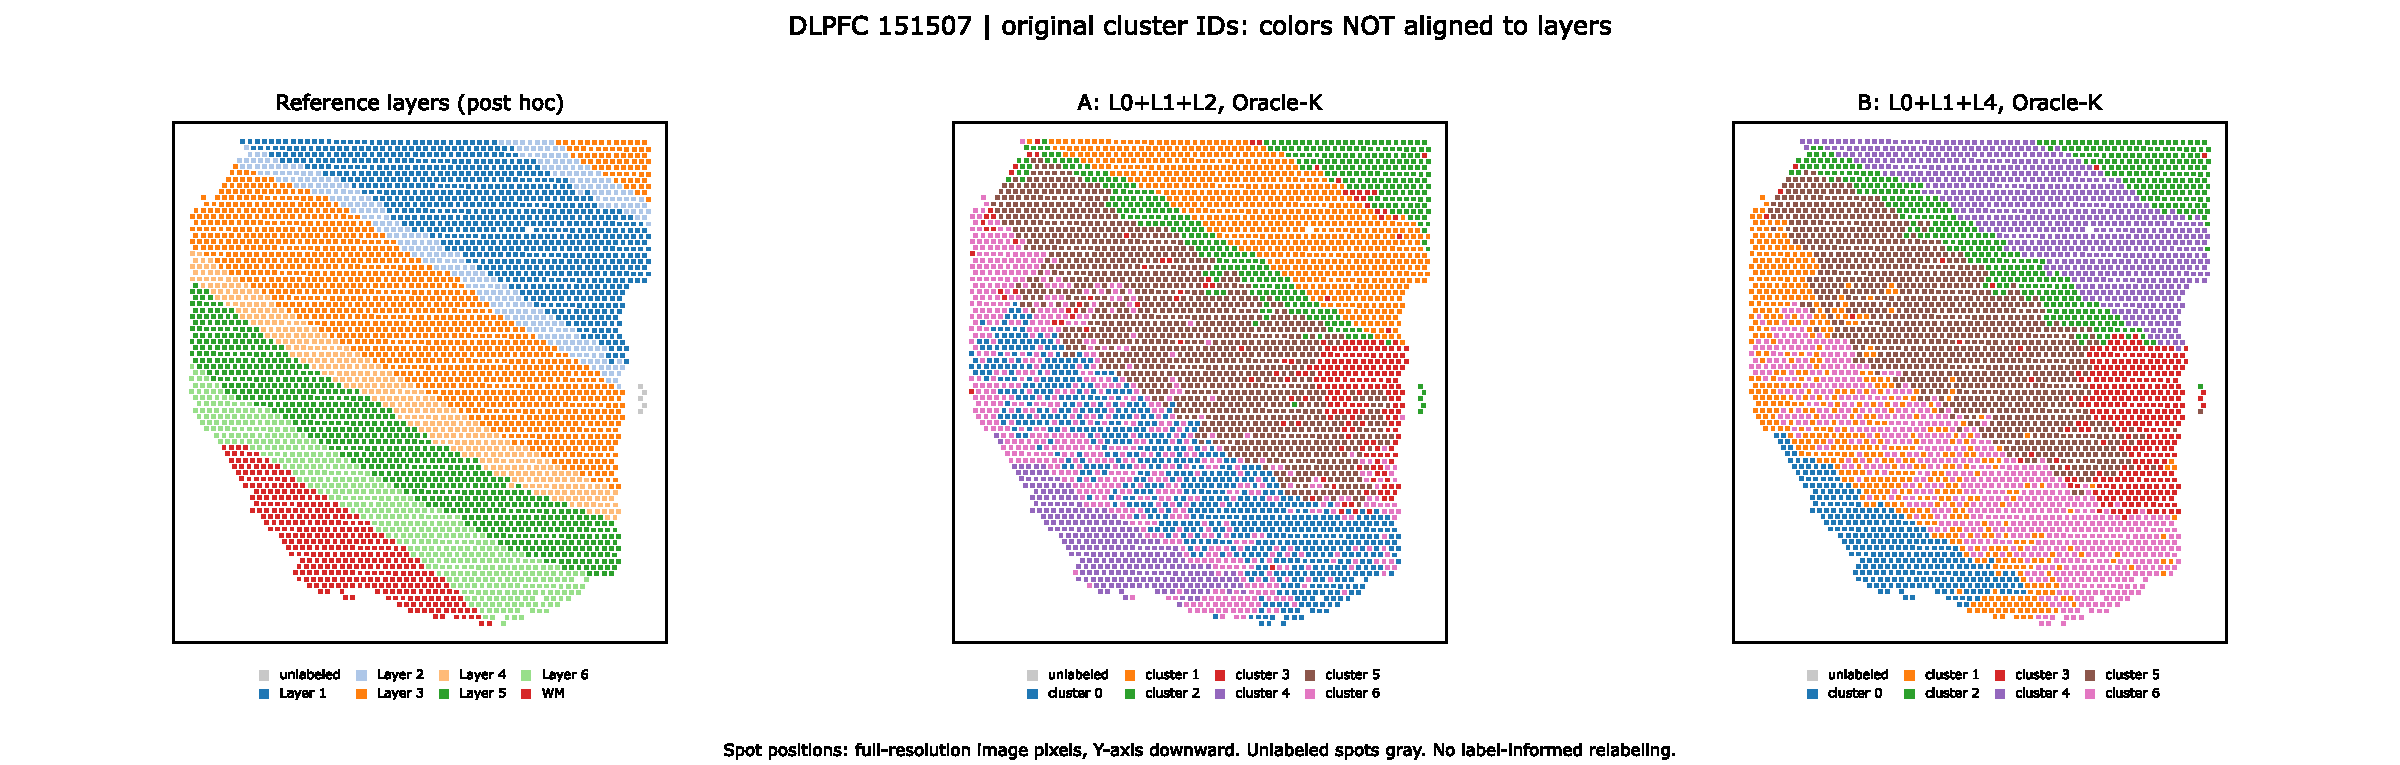
\includegraphics[width=0.98\linewidth]{E4_SOURCE_FIGURES_20261122_RELEASE/figures_pdf/151507/151507_reference_A_B_spatial.pdf}
\caption{DLPFC切片151507的参考组织层及冻结A15D、B15D原始聚类结果（E4真实SVG）。该切片按第一供体的B--A平均ARI正向代表规则选取；颜色不代表经过标签监督对齐的簇。}
\label{fig:cc-e4-151507-v1}
\end{figure}
}{%
\par\noindent\emph{[编译提示：未找到E4矢量PDF figures\_pdf/151507/151507\_reference\_A\_B\_spatial.pdf，请检查相对路径。]}\par
}
\IfFileExists{E4_SOURCE_FIGURES_20261122_RELEASE/figures_pdf/151671/151671_reference_A_B_spatial.pdf}{%
\begin{figure}[htbp]
\centering
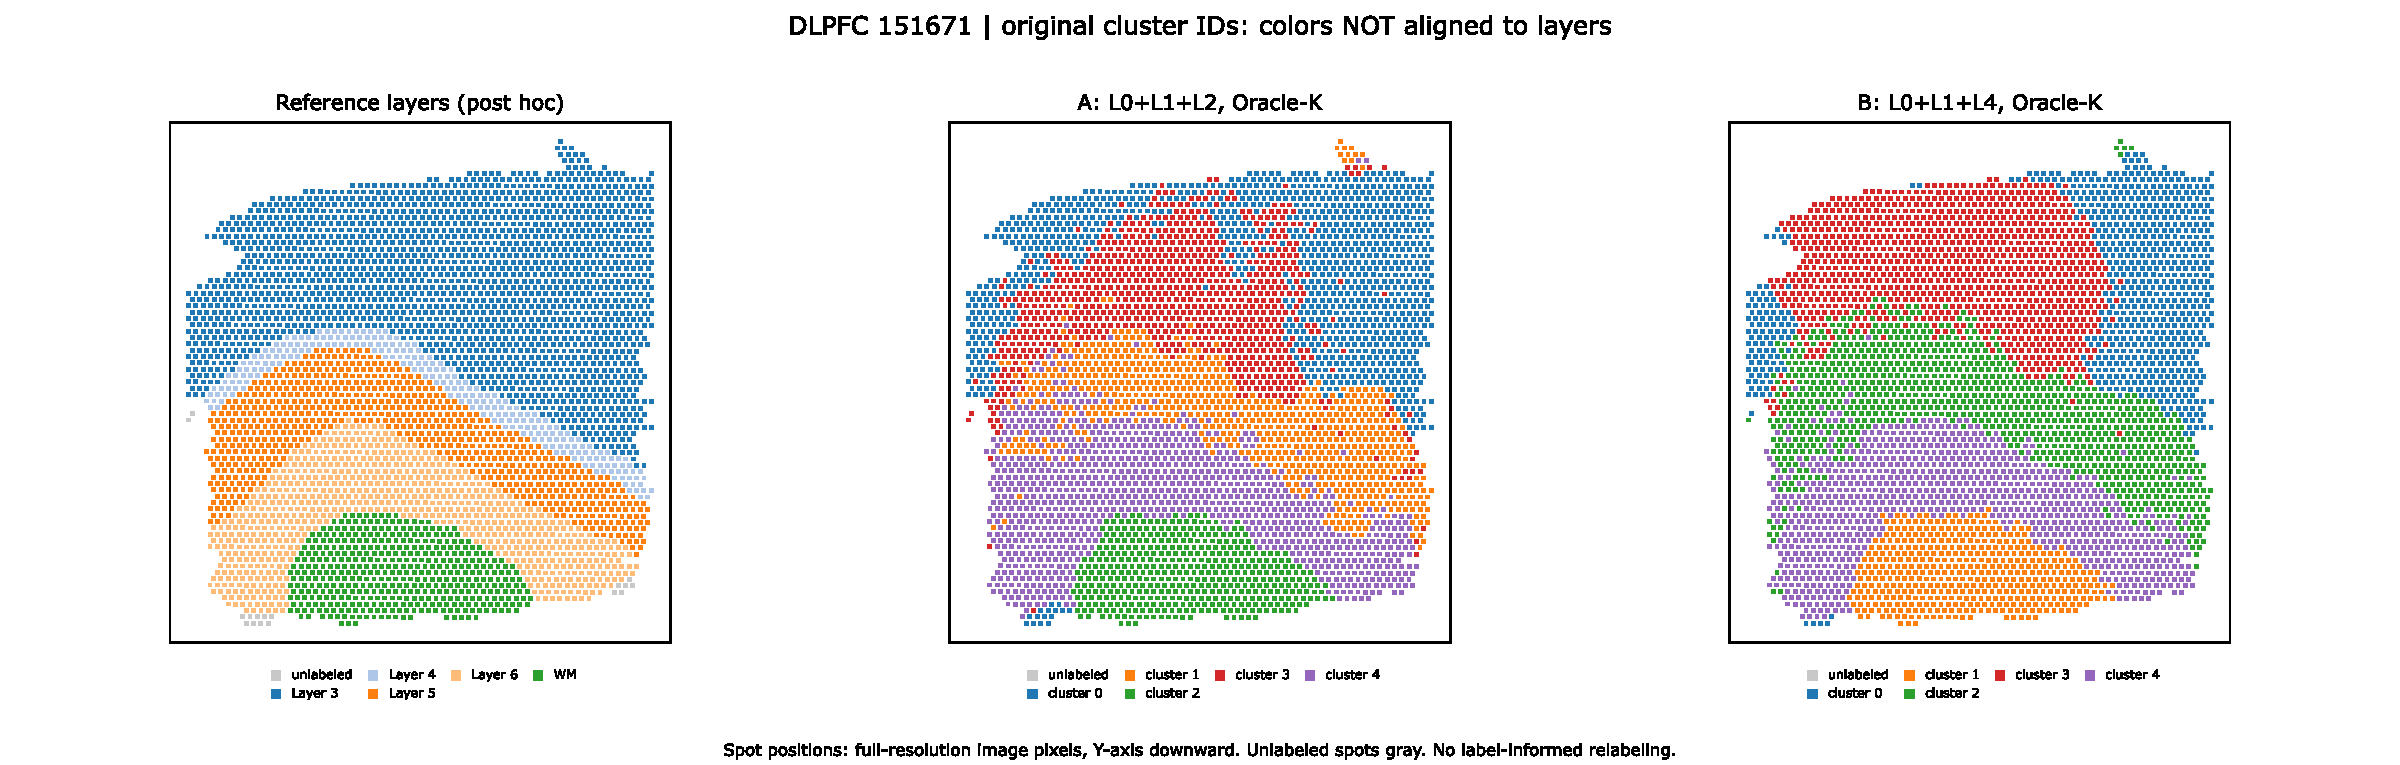
\includegraphics[width=0.98\linewidth]{E4_SOURCE_FIGURES_20261122_RELEASE/figures_pdf/151671/151671_reference_A_B_spatial.pdf}
\caption{DLPFC切片151671的参考组织层及冻结A15D、B15D原始聚类结果（E4真实SVG）。该切片按第二供体的B--A平均ARI接近零的规则选取。}
\label{fig:cc-e4-151671-v1}
\end{figure}
}{%
\par\noindent\emph{[编译提示：未找到E4矢量PDF figures\_pdf/151671/151671\_reference\_A\_B\_spatial.pdf，请检查相对路径。]}\par
}
\IfFileExists{E4_SOURCE_FIGURES_20261122_RELEASE/figures_pdf/151675/151675_reference_A_B_spatial.pdf}{%
\begin{figure}[htbp]
\centering
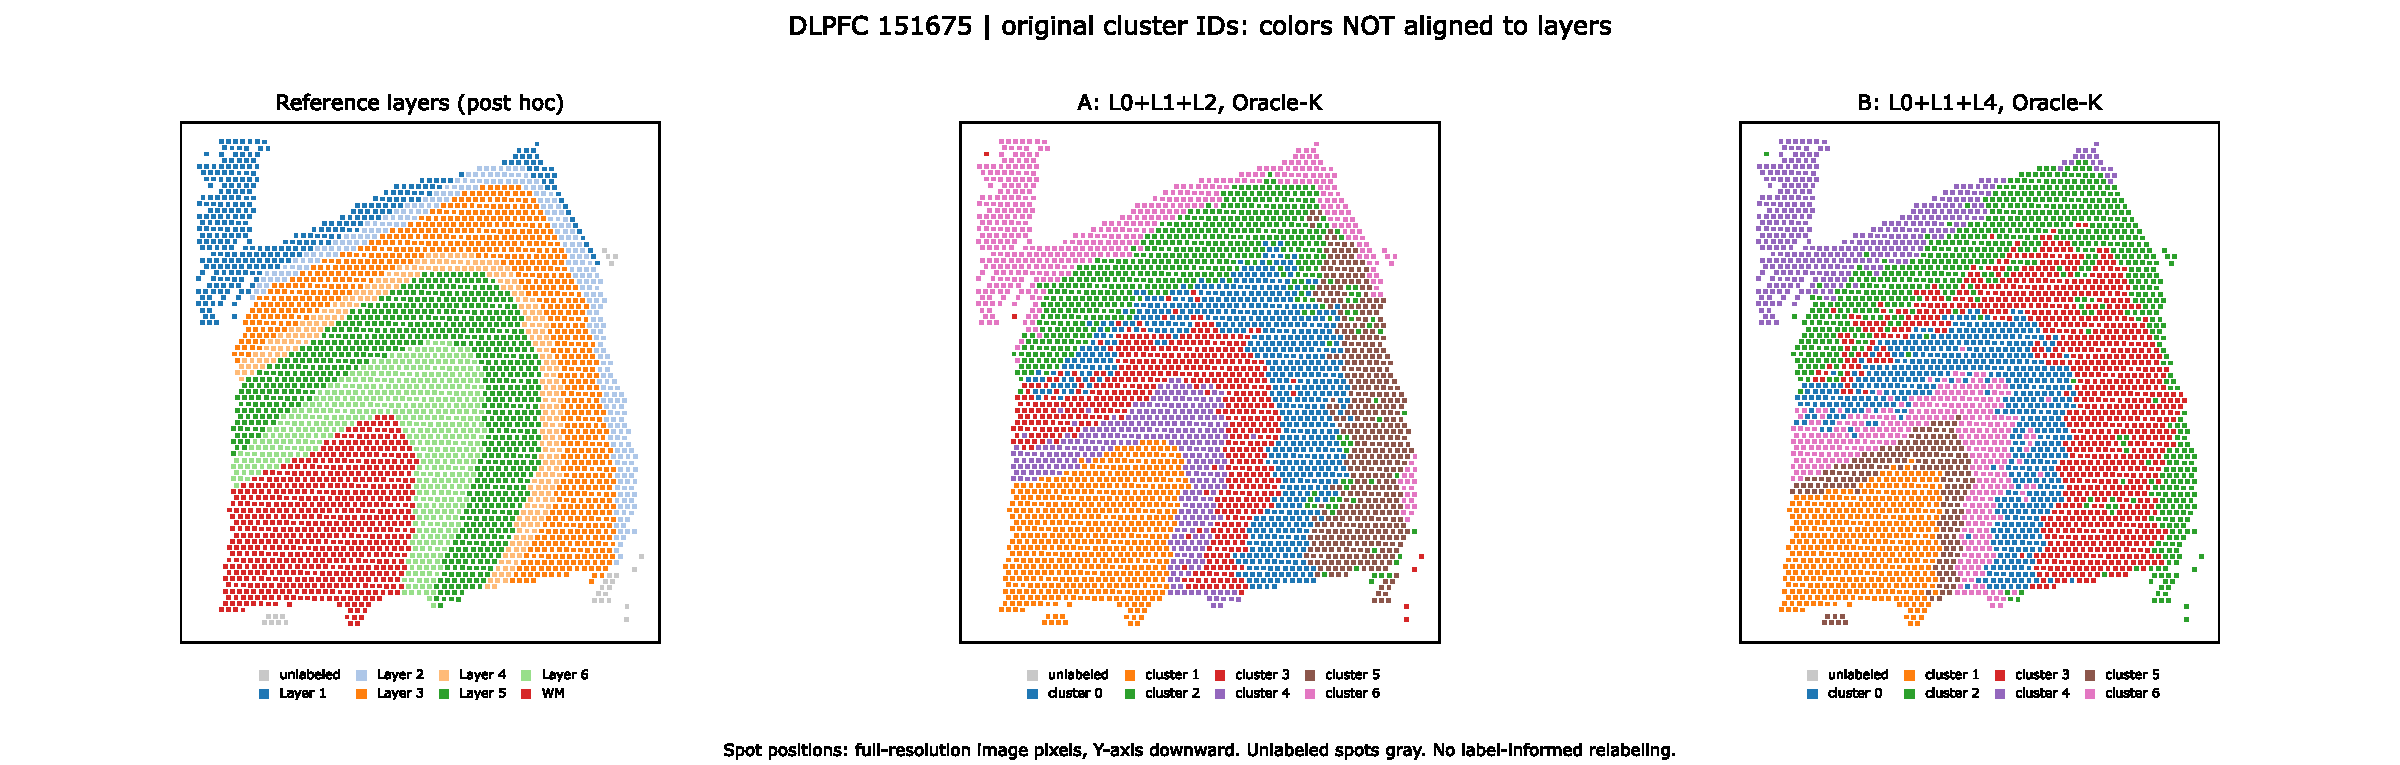
\includegraphics[width=0.98\linewidth]{E4_SOURCE_FIGURES_20261122_RELEASE/figures_pdf/151675/151675_reference_A_B_spatial.pdf}
\caption{DLPFC切片151675的参考组织层及冻结A15D、B15D原始聚类结果（E4真实SVG）。该切片按第三供体的B--A平均ARI负向代表规则选取。}
\label{fig:cc-e4-151675-v1}
\end{figure}
}{%
\par\noindent\emph{[编译提示：未找到E4矢量PDF figures\_pdf/151675/151675\_reference\_A\_B\_spatial.pdf，请检查相对路径。]}\par
}

为辅助理解皮层标记表达与空间域的关系，E4对每张切片的MOBP、PCP4、SNAP25三个标记基因分别从原始10x表达计数重新计算\texttt{log1p(10000$\times$基因UMI/spot总UMI)}，绘制统一颜色刻度范围0至6的表达图；对应原始与标准化数值保存在逐spot CSV。统一色标便于在图内比较表达分布，但图中的单个高表达区域不能直接作为人工组织层的独立验证，更不能证明某个聚类簇属于唯一确定的细胞类型。

\IfFileExists{E4_SOURCE_FIGURES_20261122_RELEASE/figures_pdf/151671/151671_MOBP_PCP4_SNAP25_expression.pdf}{%
\begin{figure}[htbp]
\centering
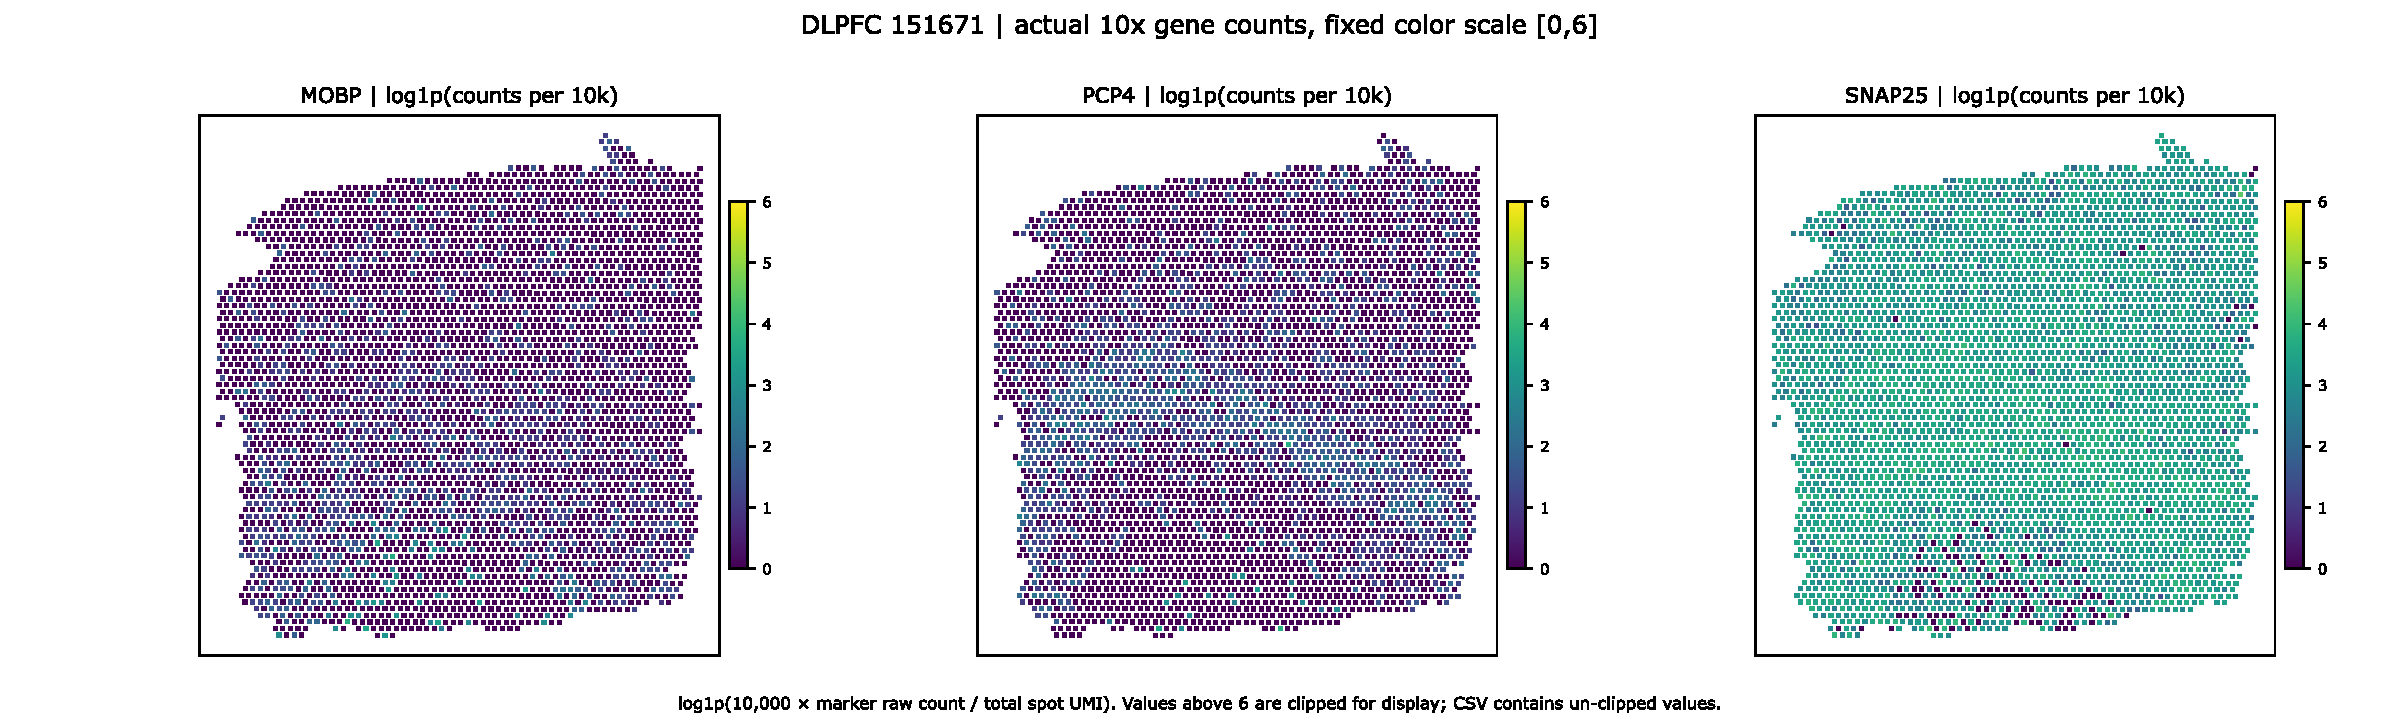
\includegraphics[width=0.98\linewidth]{E4_SOURCE_FIGURES_20261122_RELEASE/figures_pdf/151671/151671_MOBP_PCP4_SNAP25_expression.pdf}
\caption{DLPFC切片151671中MOBP、PCP4与SNAP25的原始计数归一化表达空间分布（E4真实SVG）。三图按相同归一化公式和0至6固定颜色范围展示。}
\label{fig:cc-e4-markers-151671-v1}
\end{figure}
}{%
\par\noindent\emph{[编译提示：未找到E4矢量PDF figures\_pdf/151671/151671\_MOBP\_PCP4\_SNAP25\_expression.pdf，请检查相对路径。]}\par
}

此外，E4对每张切片分别生成参考组织层与A15D/B15D原始聚类编号的完整计数交叉表及可视化，保留未标注spot的排除数量。交叉表反映不同真实层对应的聚类标签构成，避免在无监督聚类编号之间强行建立没有证据的一一对应关系。原E4独立审计报告12/12切片、36/36张SVG及36/36份CSV的产物完整性与输入SHA一致，并重新校核了marker计数和交叉表。全部36张原始SVG及其派生矢量PDF已归档，并列于附录。本章目前只把E4用作对聚类分布的直观补充，尚未对图中具体的组织形态或局部marker模式作定量陈述；若补写这类观察，须以对应的逐spot CSV和交叉表为依据。

早期旧稿曾用151671与151676举例说明单种子下边界F1正负方向的差异；此处新E4图示固定的三张代表切片遵循另一套已记录的切片级\textbf{平均ARI}代表规则，不应将这两套事后案例选择依据混同。
 

\subsection{综合讨论及本章小结}
\label{subsec:cellcharter-discussion-v1}

本章的实证结果从以下几个方面说明，多尺度空间特征聚类的评价不能仅依据单一ARI均值。

第一，25D配置及2--4层的比较与CellCharter原作者的DLPFC调参和基准重叠；本研究25D的宏平均ARI与官方单切片结果处于同一水平，但由于重复结构、GMM参数、输入文件和版本不同，这不构成严格复现。

第二，在已冻结的Oracle-K与10个技术种子条件下，5D到10D的提升在全部切片中一致；15D之后，宏平均只略有上升，约半数切片和供体D3方向相反。在固定K网格中，宏平均的尺度排序稳定。开发切片上提名的等维候选B，在其余切片和外部K-blind条件下没有复现其优势。

第三，无标签AutoK选出的簇数随切片和尺度变化很大，与参考类别数一致的情况很少。由于只做了5次重复且逐切片运行，这一结果不能直接等同于原作者推荐设置下的表现。事后ARI/NMI显示尺度表现不是简单的单调关系。

第四，严格边界F1主要随recall变化，而recall又与预测分区的碎片化程度（预测边界数量）密切相关；严格F1与1/2-hop容差F1的排序相反，不能单独用其中一个指标判断边界定位精度。

成熟基线及外部队列进一步揭示了结果的适用边界。A15D相对5D和非空间基线在6名外部患者中方向一致，但在3名ARI低于0.05的患者中差值很小。与BayesSpace的比较存在指标方向不一致的问题，并且BayesSpace和GMM的K-blind似然判据都存在明显的搜索上界问题；在Oracle-K下，A15D的ARI低于BayesSpace和Leiden。对照集也未包含原文中单切片表现最好的STAGATE。上述结论支持把本项工作定位为\textbf{基于成熟CellCharter流程、在原作者DLPFC基准之上扩展的多尺度与选K敏感性、空间边界评价及外部复核的系统实证评价}，而不是将已知特征聚合方法包装为新的基础算法。

本研究的限制主要包括：（1）DLPFC仅3名独立供体，且供体映射依据公开附录推定分组，仍需与原始元数据进一步核对；乳腺癌外部队列为6例患者，不宜作高精度群体推断。（2）25D配置由原作者在151507、151672、151673上按参考标签调出，候选B在开发切片151507上提名，这些切片都不是未接触样本。（3）部分实验使用标签类别数知情的Oracle-K，不能称为纯无监督选K表现。（4）不同空间方法的输入表征与计算路径并非完全相同；BayesSpace与GMM的K-blind判据频繁命中上界，其中BayesSpace判据与官方建议不一致；对照集未包含STAGATE。（5）AutoK每个候选K只做5次稳定性重复，未做收敛检查，且逐切片运行。（6）邻域深度和输入维度共同变化，不能据此确定因果性空间平滑机制；边界分析没有零模型基准。（7）E3d事后评分、E3b边界与容差指标、排除开发切片的汇总以及与官方结果的对照，都是在看过既有结果后进行的分析，不能倒称为前瞻注册的主终点或独立验证。（8）技术种子标准差只反映GMM初始化变异，不是生物学重复。（9）用于展示的组织学标注具有数据集特定性，外部队列并非医学诊断金标准。

综上，在遵守数据来源、独立生物学单位和完整负结果报告的前提下，现有实验已经形成从固定尺度、K敏感性、严格与容差边界到成熟基线和外部组织数据的完整描述性证据链。后续论文章节应以真实实验记录、可复算结果和可核实文献说明研究贡献，不对尚未证明的算法创新或普遍性能优势作过度推断。

\clearpage
% REV_P0 2026-11-24：由 cellcharter_study_conclusion_module_v1_20261122.tex 派生；V1保持不变。
% 按REV_P0结果改写结论1--5及局限；新增数值来源 REV_P0_20261124/derived/T1--T8。
% CellCharter研究专题结论与展望模块（非整篇硕士学位论文总论终稿）
% 对应真实E1/E2,E3c,E3d,E3b,E5a,E5b结果；不预设新算法或统计显著性。
\section{本研究的结论与展望}
\label{sec:cc-conclusion-module-v1}

\subsection{主要实证结论}
本研究在成熟CellCharter空间邻域表示与聚类流程基础上，围绕特征深度、聚类数确定、空间边界以及跨组织评价开展了系统的计算实验。DLPFC部分包含12张切片、3名独立供体；外部数据为6名乳腺癌患者。CellCharter原作者已在同一DLPFC数据上完成基准比较，并对2--4层邻域做过调参\cite{varrone2024,cellcharteranalyses2024}，本研究的25D配置即其最终配置。因此，本研究的贡献是在该基准之上作扩展性的实证评价，不是新方法，也不是对“邻域层数影响ARI”的首次发现。

第一，在固定Oracle-K条件下，每张切片先平均10个技术种子，再对12张切片等权汇总：累计邻域特征从5D增加到25D时，ARI由0.3051提高至0.4418，NMI由0.4133提高至0.5982。其中5D到10D的提升在12/12张切片上方向一致；15D之后，宏平均只略有上升，约半数切片以及供体D3的方向相反。本研究25D的宏平均ARI（0.4418）与原作者官方单切片结果（0.4438）处于同一水平，但两者在重复结构、GMM参数、输入文件和软件版本上存在差异，不构成严格复现。

第二，等维候选B15D（$L_0+L_1+L_4$）是在开发切片151507上看到正向结果后提名的。按预设口径，B相对A15D的12切片平均ARI变化为$+0.0033$；排除两张开发切片后，其余10张切片的平均变化为$-0.0035$（事后汇总）。按供体看，D1为正、D3为负；在外部6名患者的K-blind条件下为$-0.0364$（1/6为正）。B应记为开发集提名、扩展评价中未获稳定支持的负结果。

第三，聚类数设置改变了尺度比较的解释。在E3c预设固定K网格中，每个K下宏平均ARI的尺度排序都是25D $>$ 20D $>$ 15D $>$ 10D，但这种扫描不是无标签模型选择。E3d逐切片AutoK在48个切片--尺度组合中，有10项触及冻结的K=2至10搜索区间边界，选中K与参考类别数一致的情况在每个尺度下只有1/12。本研究每个候选K只做5次重复，少于原作者的10次，且原作者是联合选K。事后评价中，20D的12切片ARI和NMI均值较高（0.4311与0.5942），但供体之间不一致；由于不同尺度实际选中的K不同，这一结果不能作为推荐配置。

第四，空间边界评价呈现与整体聚类指标不同的趋势，以下均为事后分析。严格0-hop F1在5D与10D之间基本持平（0.1441与0.1446），此后下降至25D的0.1179；2-hop容差F1则由0.2863上升至0.5333。严格F1的变化主要来自recall：浅层表示的预测更碎片化，预测边界边数是参考边界的6.4倍（5D），而25D为1.4倍。因此，严格F1较高不等于定位更精确，容差F1较高也不能代替严格定位。这是一项指标定义敏感性观察，不等于已经通过实验确定了“过度平滑”的生物学原因。

第五，与非空间GMM、Leiden及成熟空间方法BANKSY、BayesSpace比较时，CellCharter的表现取决于数据、K策略和指标，不能宣称对所有空间方法普遍占优。本研究冻结的BayesSpace K-blind判据与官方建议的elbow判断不一致\cite{bayesspacevignette}，在DLPFC的36项中有28项、乳腺癌的18项中有18项命中搜索上界；非空间GMM的BIC判据在DLPFC也有32/36项命中上界。这些结果全部保留，但会降低K-blind对比的可比性。此外，对照集未包含原文中单切片表现最好的STAGATE。

第六，在6名乳腺癌患者的外部K-blind评价中，A15D相对5D基础配置的ARI宏平均差约为$+0.0458$、NMI差约为$+0.0583$，两项指标在6/6例患者上方向一致；但在3名ARI低于0.05的患者中，这些差值与种子波动处于同一量级。与BayesSpace比较时，A15D的ARI仅在4/6例患者较高，患者平均NMI差约为$-0.0139$；在Oracle-K下，A15D的ARI低于BayesSpace和Leiden。此结果是将相同研究流程重新用于新组织队列所得的观察，不是将DLPFC已训练模型直接泛化到乳腺癌。

\subsection{研究局限}
本研究在解释层面主要受到以下因素限制：
\begin{enumerate}
  \item DLPFC仅3位供体且存在供体内多个切片，乳腺癌仅6名患者，均不足以支持高精度总体推断。
  \item 25D配置由原作者按参考标签在3张切片上调出，候选B在开发切片上提名，这些切片都不是未接触样本；DLPFC部分参考标注来源及旧开发样本的数据卫生问题需在论文数据来源中保留。
  \item Oracle-K使用参考类别数，不能代表真正未知类别数的无标签应用。
  \item 部分实验中的邻域深度与输入维度同步变化；成熟基线的预处理、计算预算及K-blind规则又存在方法间差异，其中BayesSpace与GMM的似然判据频繁命中上界，对照集未包含STAGATE。
  \item AutoK只做5次稳定性重复，且逐切片运行。
  \item E3d的后验ARI/NMI、E3b的边界与容差分析、排除开发切片的汇总，以及与官方结果的对照，都是在已有模型结果之后追加的事后分析。
  \item 技术种子标准差只反映GMM初始化变异，不是生物学重复。
  \item 病理区域标签与皮层层级标签的语义不同，不能将跨组织ARI绝对值直接对比。
\end{enumerate}

因此，本文展示的是基于已知模型的系统实证评价与可重复的研究流程，而非已验证的新核心聚类算法。在没有更多独立数据和精确因果控制前，不能对边界变化原因、参数最优性或临床应用价值作肯定性普遍结论。

\subsection{后续工作展望}
后续研究可以在以下方向展开：在更多独立供体和组织类型上检验当前观察的适用性；按各方法官方建议的选K方式（例如BayesSpace的elbow判断）以及足够的稳定性重复次数重新设计K-blind对照，并纳入STAGATE等强基线；使用明确的等维和等计算预算对照，进一步区分尺度范围、特征维数和模型随机性；为边界指标建立零模型基准，并结合组织层过渡区域的标注不确定性，避免仅凭单一参考标签和单一指标判断算法表现。

以上属于对当前研究局限的未来研究方向，不表示本研究已经执行了上述扩展。本文当前工作已经完成相应冻结实验及事后分析，毕业论文写作应首先完整呈现已发生的研究事实，而不将计划工作当作已经取得的结果。

\clearpage
\IfFileExists{E4_SOURCE_FIGURES_20261122_RELEASE/figures_pdf/151507/151507_reference_A_B_spatial.pdf}{%
\clearpage
\appendix
% E4 full original-plots appendix LAYOUT V2. All 36 original figures remain.
% NOTE: Nonfloating figure blocks ensure each subsection title precedes its figures.
% Scientific content, figure paths, captions, labels and if-exists fallbacks retained.
% E4 full original-plots appendix V1. Figures require real vector PDFs derived from source SVGs.
% Existing predictions, labels and marker CSVs must remain unchanged.
\section{E4全12切片原始图件}
\label{sec:cc-e4-appendix-v1}
此附录依据事前固定的12切片完整E4清单列出空间聚类、标记基因与交叉计数图。所有图对应seed22911及Oracle-K的A15D/B15D，三个供体的12张切片不构成12个独立生物学重复。原始SVG与CSV必须另行核验，只有已经从真实SVG无重绘转换得到的矢量PDF才显示于正文；否则保留待插图提示。

\subsection{DLPFC切片151507}
\IfFileExists{E4_SOURCE_FIGURES_20261122_RELEASE/figures_pdf/151507/151507_reference_A_B_spatial.pdf}{%
\par\noindent\begin{minipage}{\linewidth}
\centering
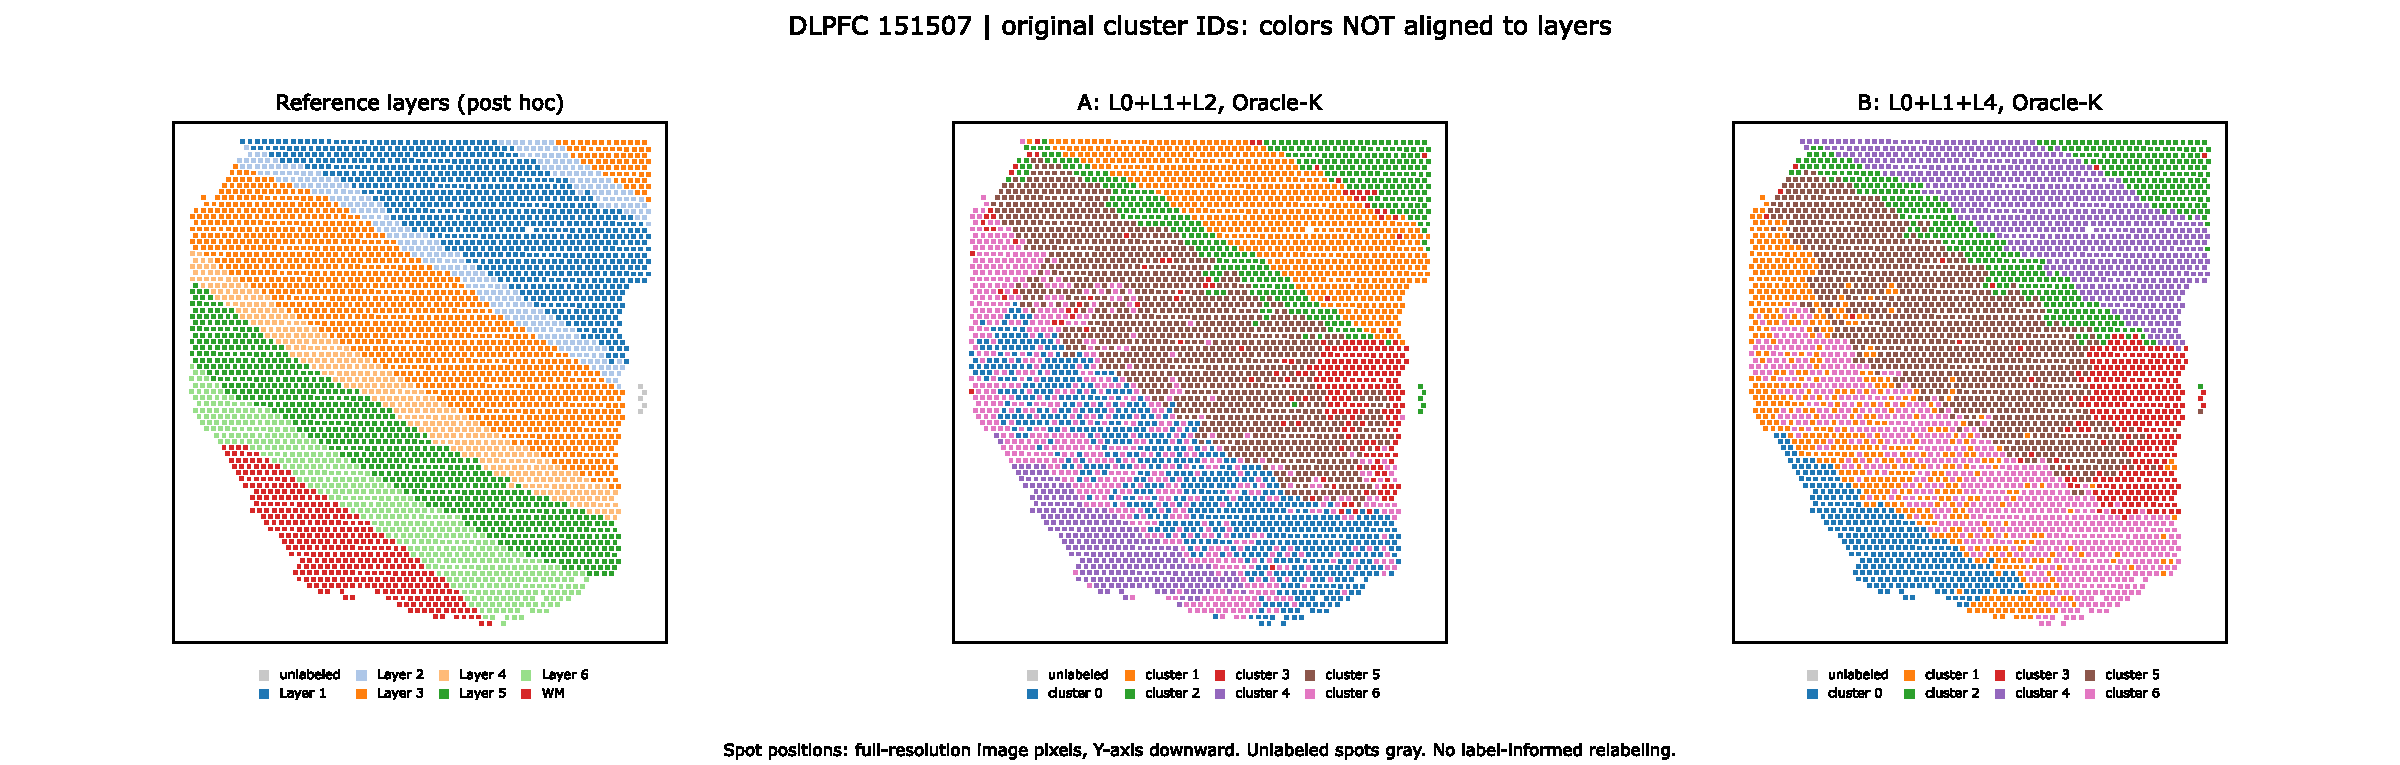
\includegraphics[width=0.97\linewidth,height=0.72\textheight,keepaspectratio]{E4_SOURCE_FIGURES_20261122_RELEASE/figures_pdf/151507/151507_reference_A_B_spatial.pdf}
\captionof{figure}{DLPFC切片151507：参考层与A/B原始聚类三联图（原始E4图件转换的矢量PDF；聚类编号未根据参考标签重排）。}
\label{fig:cc-e4-app-151507-map}
\end{minipage}\par\medskip
}{%
\par\noindent\emph{[待插入原始E4图件：151507_reference_A_B_spatial.svg]}\par
}
\IfFileExists{E4_SOURCE_FIGURES_20261122_RELEASE/figures_pdf/151507/151507_MOBP_PCP4_SNAP25_expression.pdf}{%
\par\noindent\begin{minipage}{\linewidth}
\centering
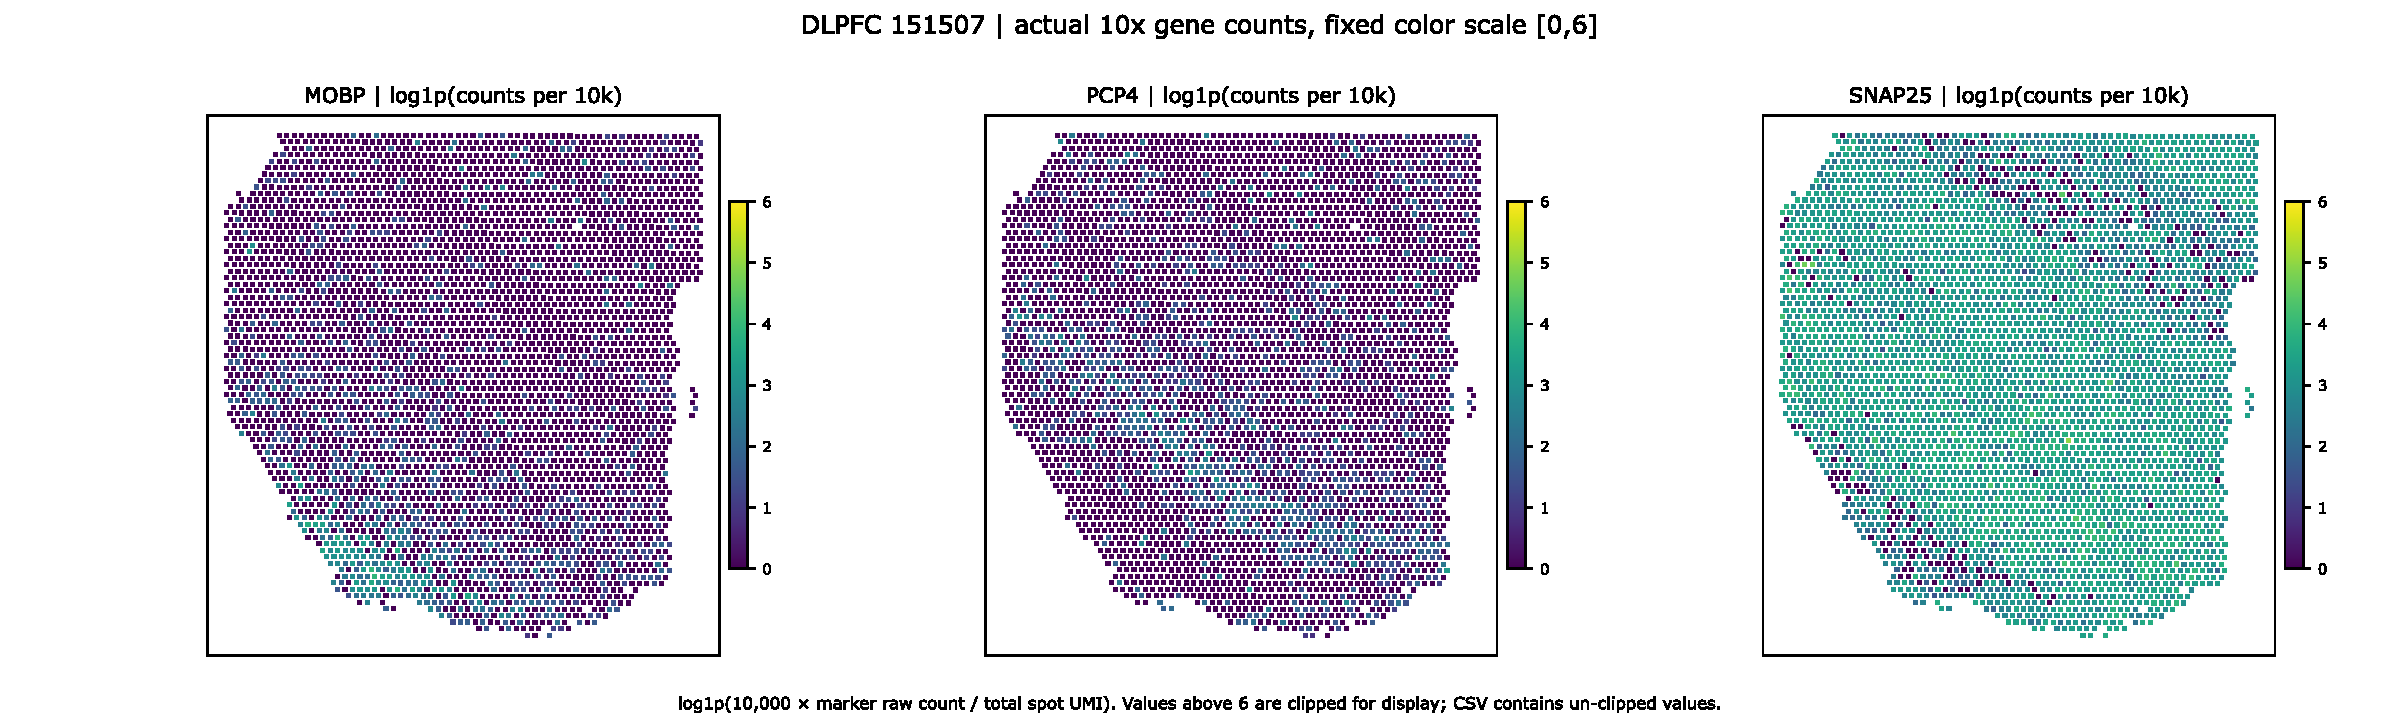
\includegraphics[width=0.97\linewidth,height=0.72\textheight,keepaspectratio]{E4_SOURCE_FIGURES_20261122_RELEASE/figures_pdf/151507/151507_MOBP_PCP4_SNAP25_expression.pdf}
\captionof{figure}{DLPFC切片151507：MOBP/PCP4/SNAP25表达三联图（原始E4图件转换的矢量PDF；聚类编号未根据参考标签重排）。}
\label{fig:cc-e4-app-151507-markers}
\end{minipage}\par\medskip
}{%
\par\noindent\emph{[待插入原始E4图件：151507_MOBP_PCP4_SNAP25_expression.svg]}\par
}
\IfFileExists{E4_SOURCE_FIGURES_20261122_RELEASE/figures_pdf/151507/151507_reference_A_B_confusion.pdf}{%
\par\noindent\begin{minipage}{\linewidth}
\centering
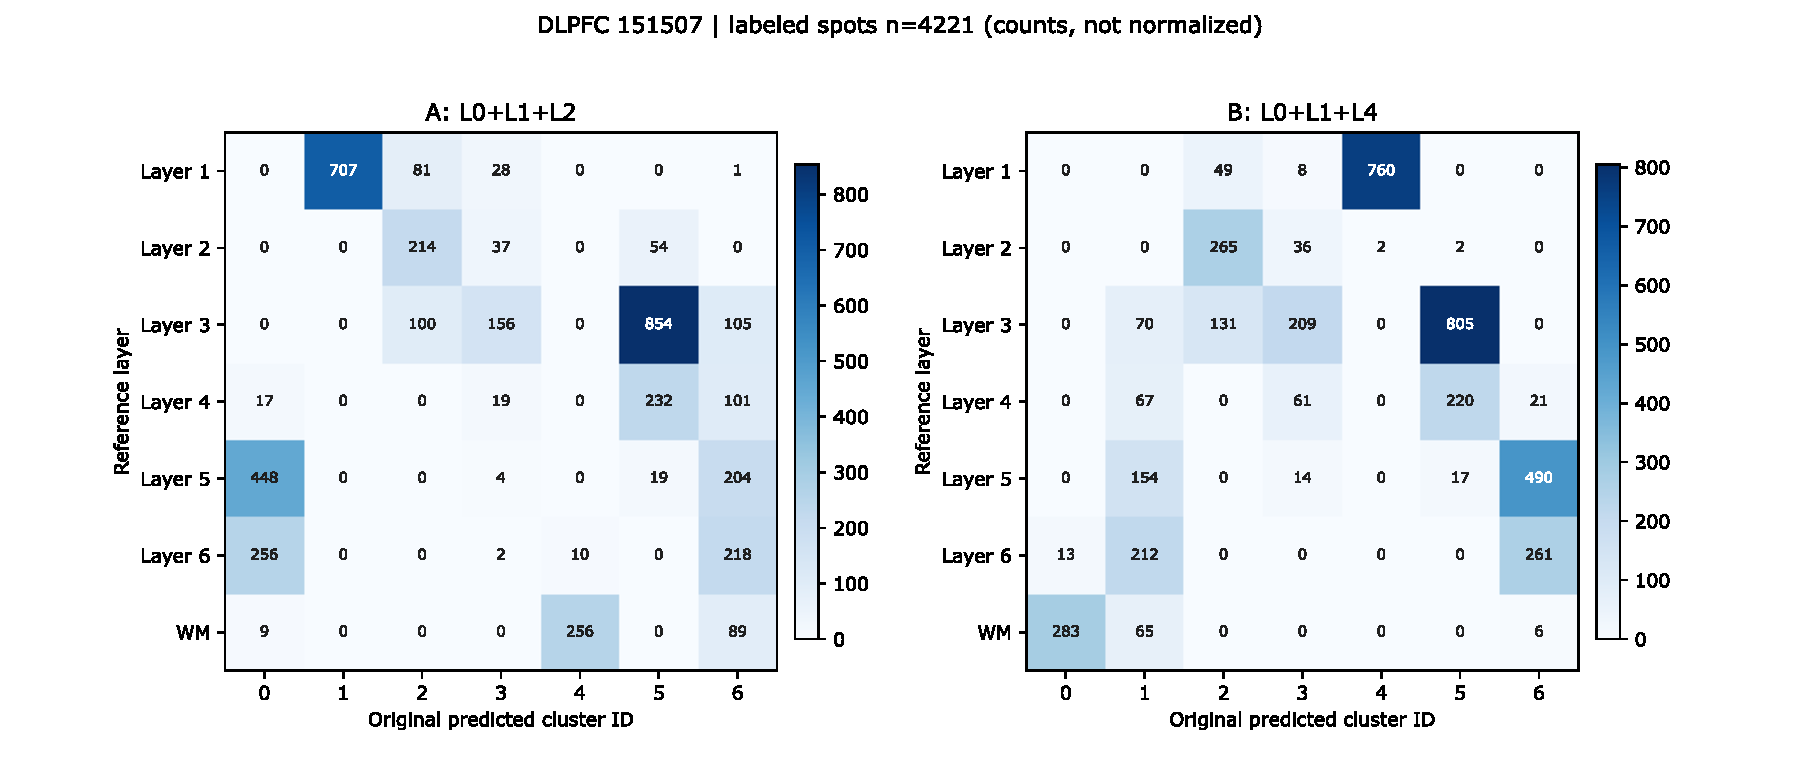
\includegraphics[width=0.97\linewidth,height=0.72\textheight,keepaspectratio]{E4_SOURCE_FIGURES_20261122_RELEASE/figures_pdf/151507/151507_reference_A_B_confusion.pdf}
\captionof{figure}{DLPFC切片151507：参考层与A/B簇交叉计数图（原始E4图件转换的矢量PDF；聚类编号未根据参考标签重排）。}
\label{fig:cc-e4-app-151507-confusion}
\end{minipage}\par\medskip
}{%
\par\noindent\emph{[待插入原始E4图件：151507_reference_A_B_confusion.svg]}\par
}
\subsection{DLPFC切片151508}
\IfFileExists{E4_SOURCE_FIGURES_20261122_RELEASE/figures_pdf/151508/151508_reference_A_B_spatial.pdf}{%
\par\noindent\begin{minipage}{\linewidth}
\centering
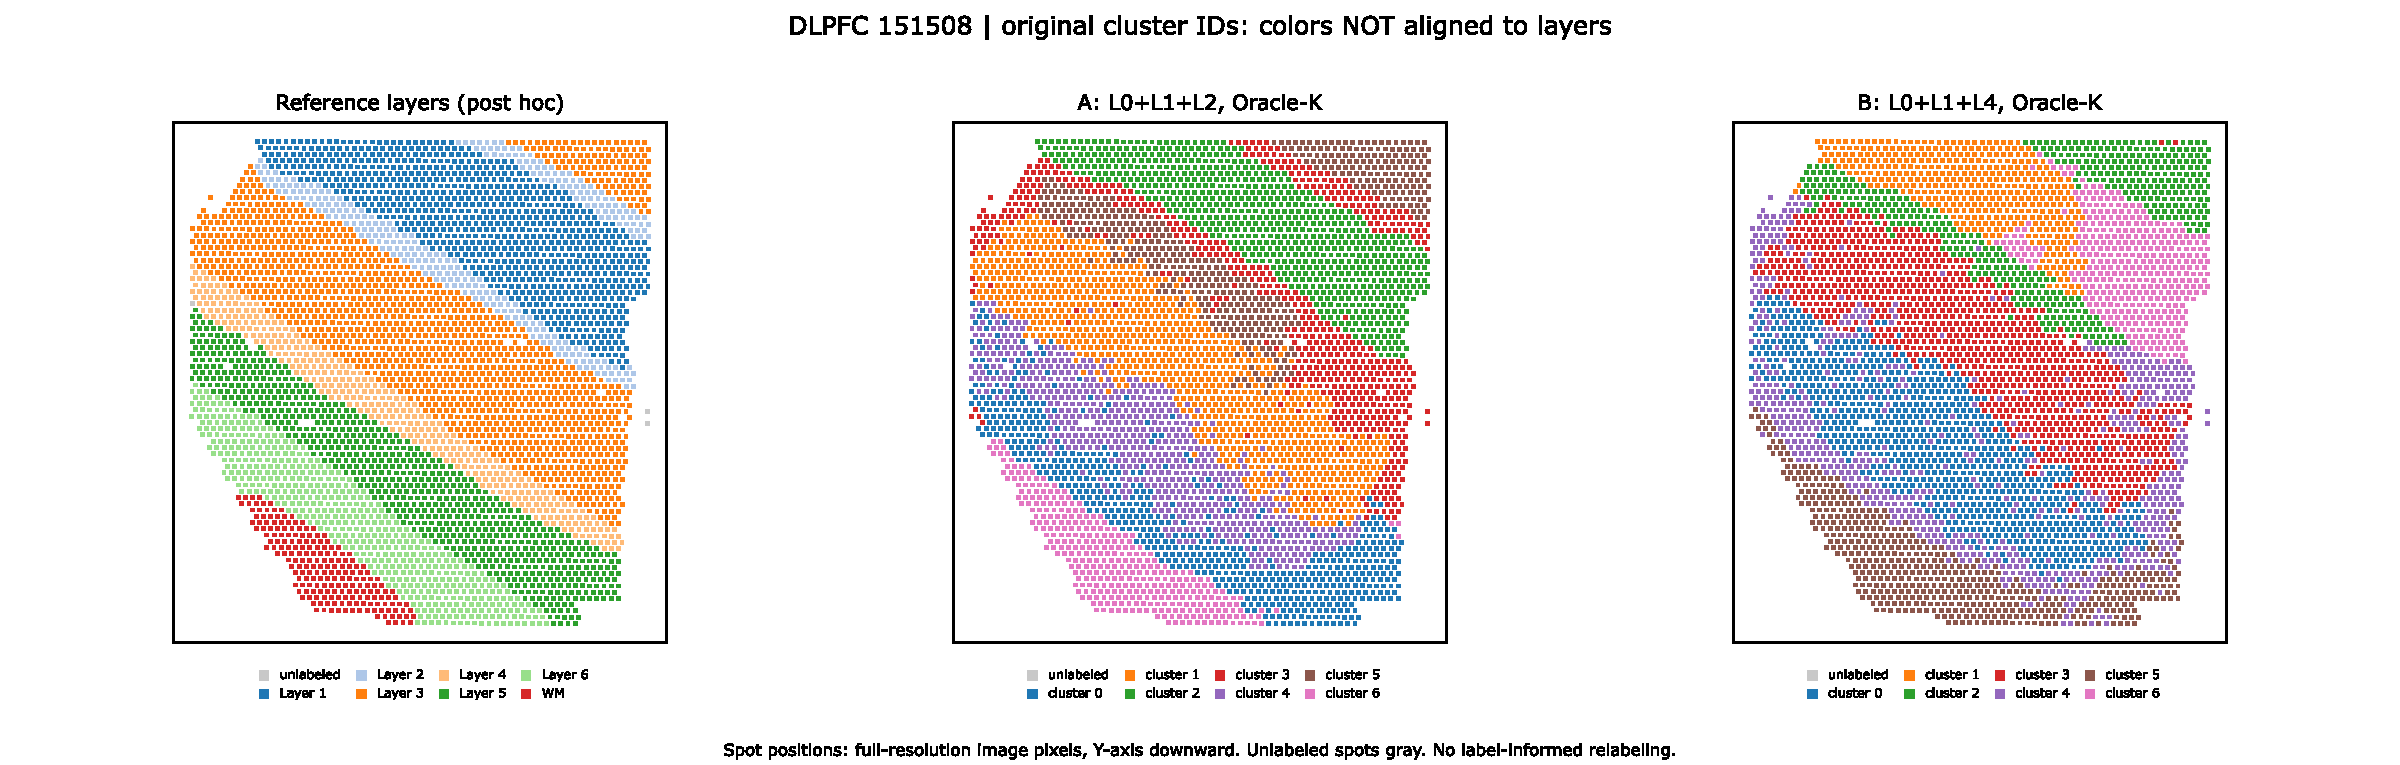
\includegraphics[width=0.97\linewidth,height=0.72\textheight,keepaspectratio]{E4_SOURCE_FIGURES_20261122_RELEASE/figures_pdf/151508/151508_reference_A_B_spatial.pdf}
\captionof{figure}{DLPFC切片151508：参考层与A/B原始聚类三联图（原始E4图件转换的矢量PDF；聚类编号未根据参考标签重排）。}
\label{fig:cc-e4-app-151508-map}
\end{minipage}\par\medskip
}{%
\par\noindent\emph{[待插入原始E4图件：151508_reference_A_B_spatial.svg]}\par
}
\IfFileExists{E4_SOURCE_FIGURES_20261122_RELEASE/figures_pdf/151508/151508_MOBP_PCP4_SNAP25_expression.pdf}{%
\par\noindent\begin{minipage}{\linewidth}
\centering
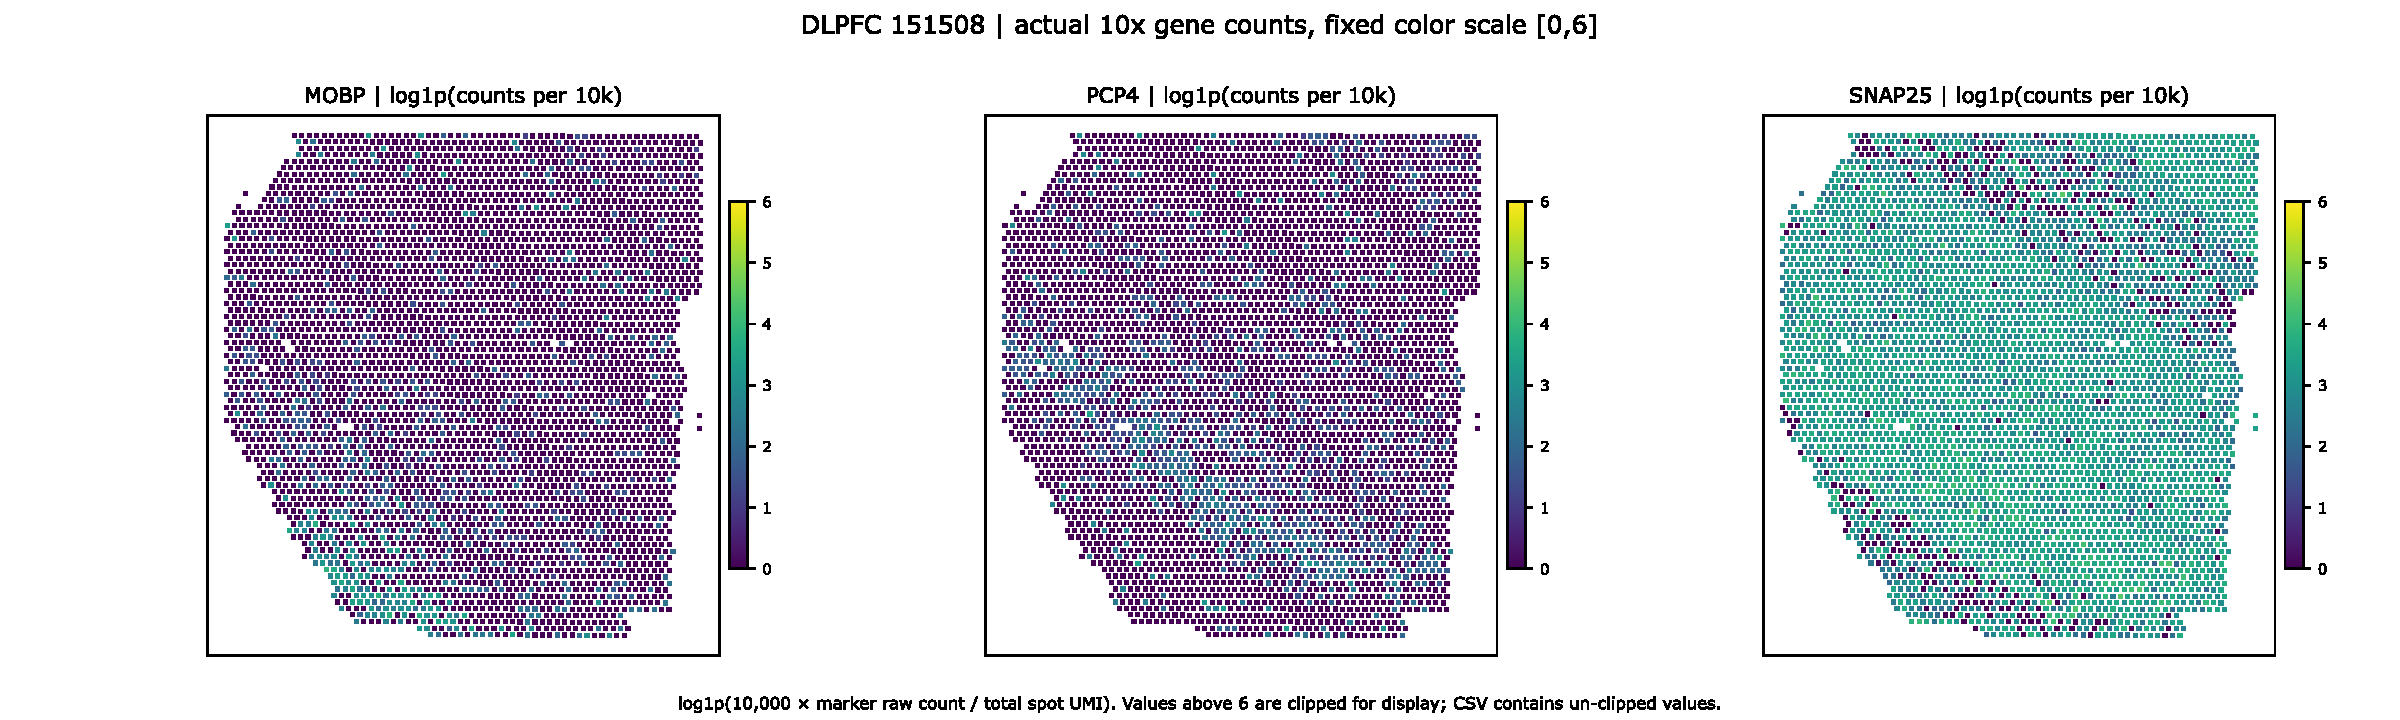
\includegraphics[width=0.97\linewidth,height=0.72\textheight,keepaspectratio]{E4_SOURCE_FIGURES_20261122_RELEASE/figures_pdf/151508/151508_MOBP_PCP4_SNAP25_expression.pdf}
\captionof{figure}{DLPFC切片151508：MOBP/PCP4/SNAP25表达三联图（原始E4图件转换的矢量PDF；聚类编号未根据参考标签重排）。}
\label{fig:cc-e4-app-151508-markers}
\end{minipage}\par\medskip
}{%
\par\noindent\emph{[待插入原始E4图件：151508_MOBP_PCP4_SNAP25_expression.svg]}\par
}
\IfFileExists{E4_SOURCE_FIGURES_20261122_RELEASE/figures_pdf/151508/151508_reference_A_B_confusion.pdf}{%
\par\noindent\begin{minipage}{\linewidth}
\centering
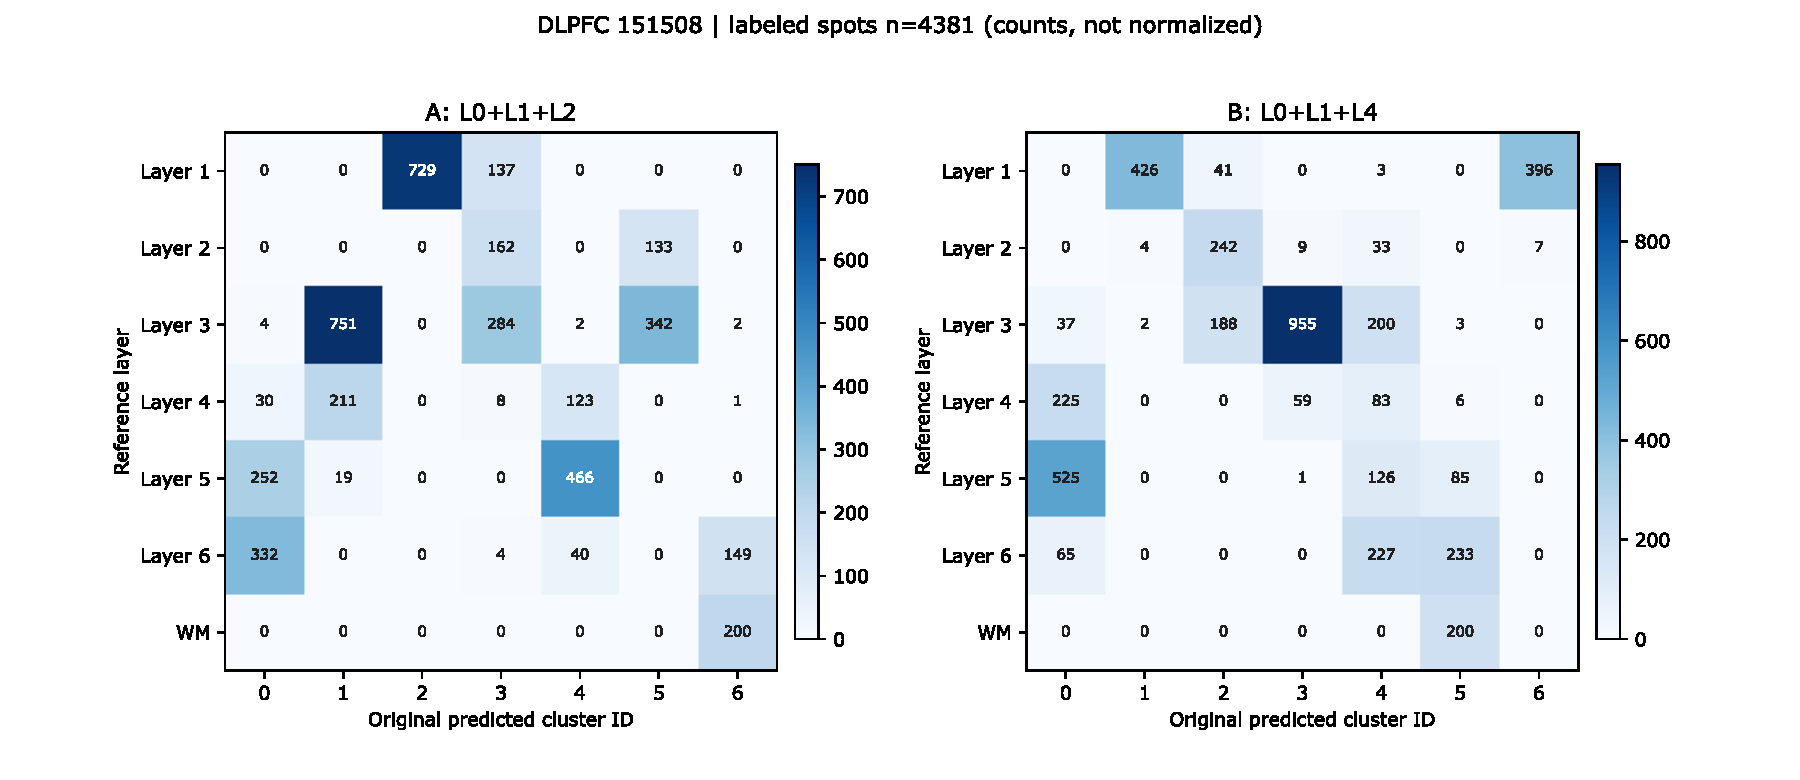
\includegraphics[width=0.97\linewidth,height=0.72\textheight,keepaspectratio]{E4_SOURCE_FIGURES_20261122_RELEASE/figures_pdf/151508/151508_reference_A_B_confusion.pdf}
\captionof{figure}{DLPFC切片151508：参考层与A/B簇交叉计数图（原始E4图件转换的矢量PDF；聚类编号未根据参考标签重排）。}
\label{fig:cc-e4-app-151508-confusion}
\end{minipage}\par\medskip
}{%
\par\noindent\emph{[待插入原始E4图件：151508_reference_A_B_confusion.svg]}\par
}
\subsection{DLPFC切片151509}
\IfFileExists{E4_SOURCE_FIGURES_20261122_RELEASE/figures_pdf/151509/151509_reference_A_B_spatial.pdf}{%
\par\noindent\begin{minipage}{\linewidth}
\centering
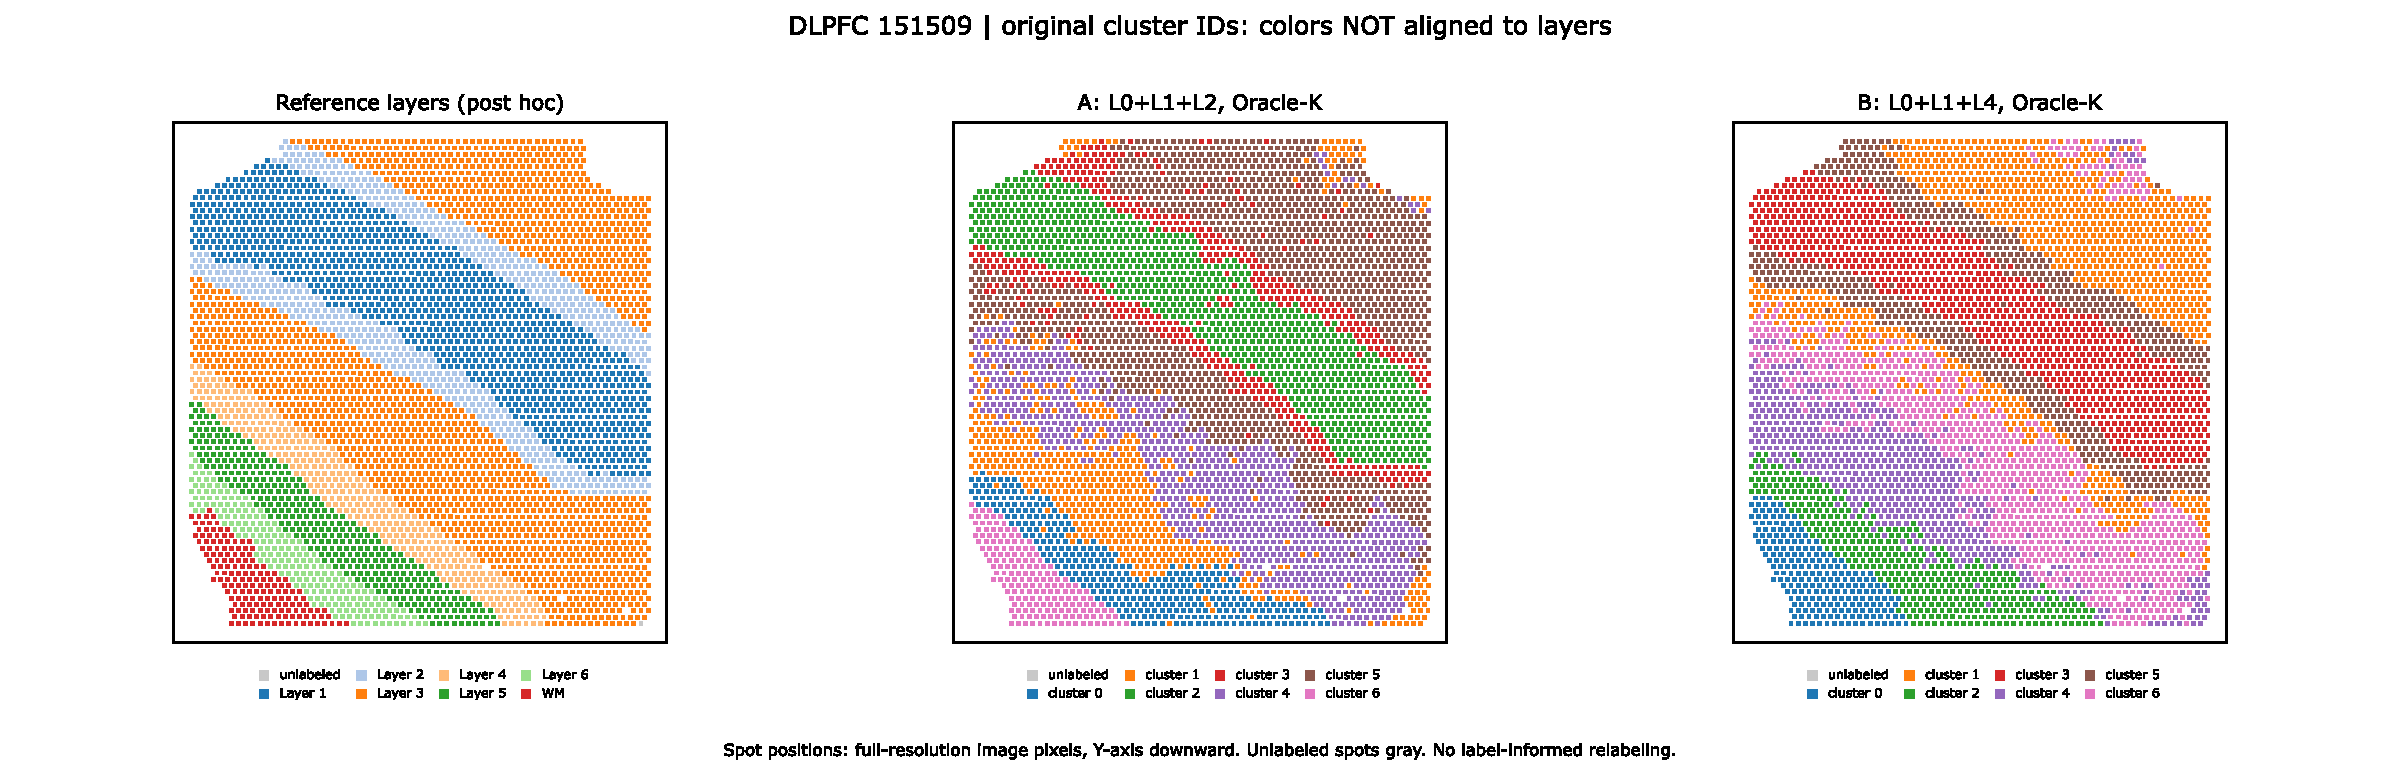
\includegraphics[width=0.97\linewidth,height=0.72\textheight,keepaspectratio]{E4_SOURCE_FIGURES_20261122_RELEASE/figures_pdf/151509/151509_reference_A_B_spatial.pdf}
\captionof{figure}{DLPFC切片151509：参考层与A/B原始聚类三联图（原始E4图件转换的矢量PDF；聚类编号未根据参考标签重排）。}
\label{fig:cc-e4-app-151509-map}
\end{minipage}\par\medskip
}{%
\par\noindent\emph{[待插入原始E4图件：151509_reference_A_B_spatial.svg]}\par
}
\IfFileExists{E4_SOURCE_FIGURES_20261122_RELEASE/figures_pdf/151509/151509_MOBP_PCP4_SNAP25_expression.pdf}{%
\par\noindent\begin{minipage}{\linewidth}
\centering
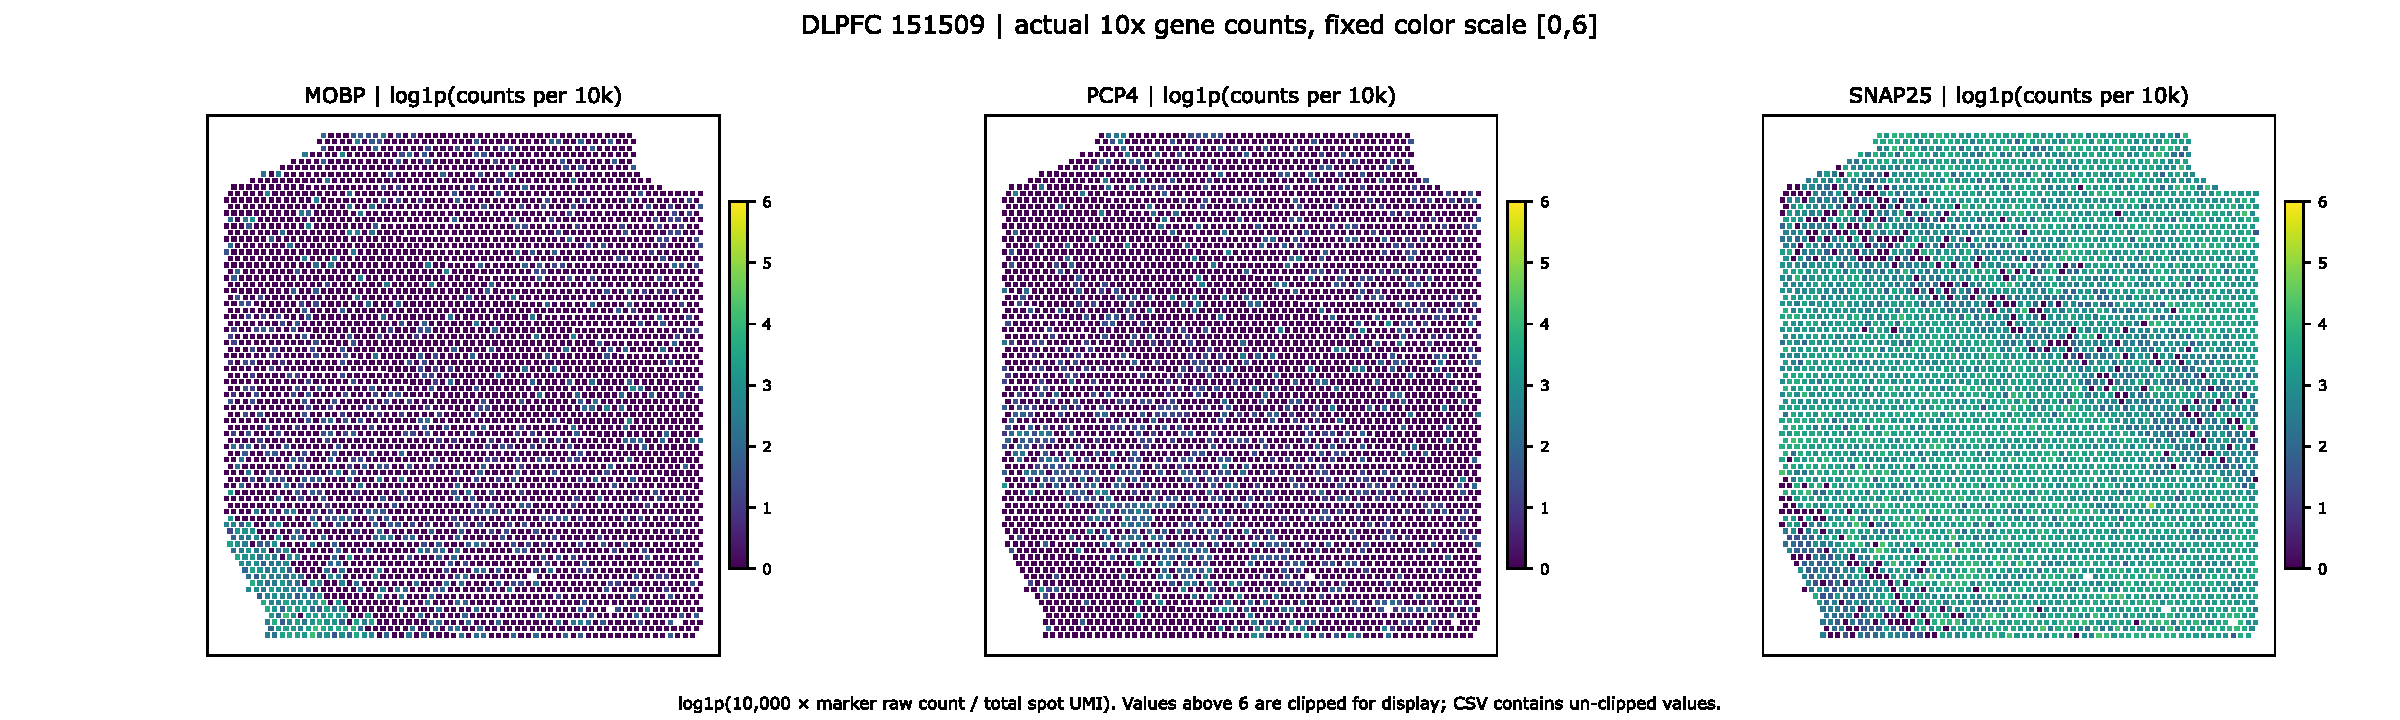
\includegraphics[width=0.97\linewidth,height=0.72\textheight,keepaspectratio]{E4_SOURCE_FIGURES_20261122_RELEASE/figures_pdf/151509/151509_MOBP_PCP4_SNAP25_expression.pdf}
\captionof{figure}{DLPFC切片151509：MOBP/PCP4/SNAP25表达三联图（原始E4图件转换的矢量PDF；聚类编号未根据参考标签重排）。}
\label{fig:cc-e4-app-151509-markers}
\end{minipage}\par\medskip
}{%
\par\noindent\emph{[待插入原始E4图件：151509_MOBP_PCP4_SNAP25_expression.svg]}\par
}
\IfFileExists{E4_SOURCE_FIGURES_20261122_RELEASE/figures_pdf/151509/151509_reference_A_B_confusion.pdf}{%
\par\noindent\begin{minipage}{\linewidth}
\centering
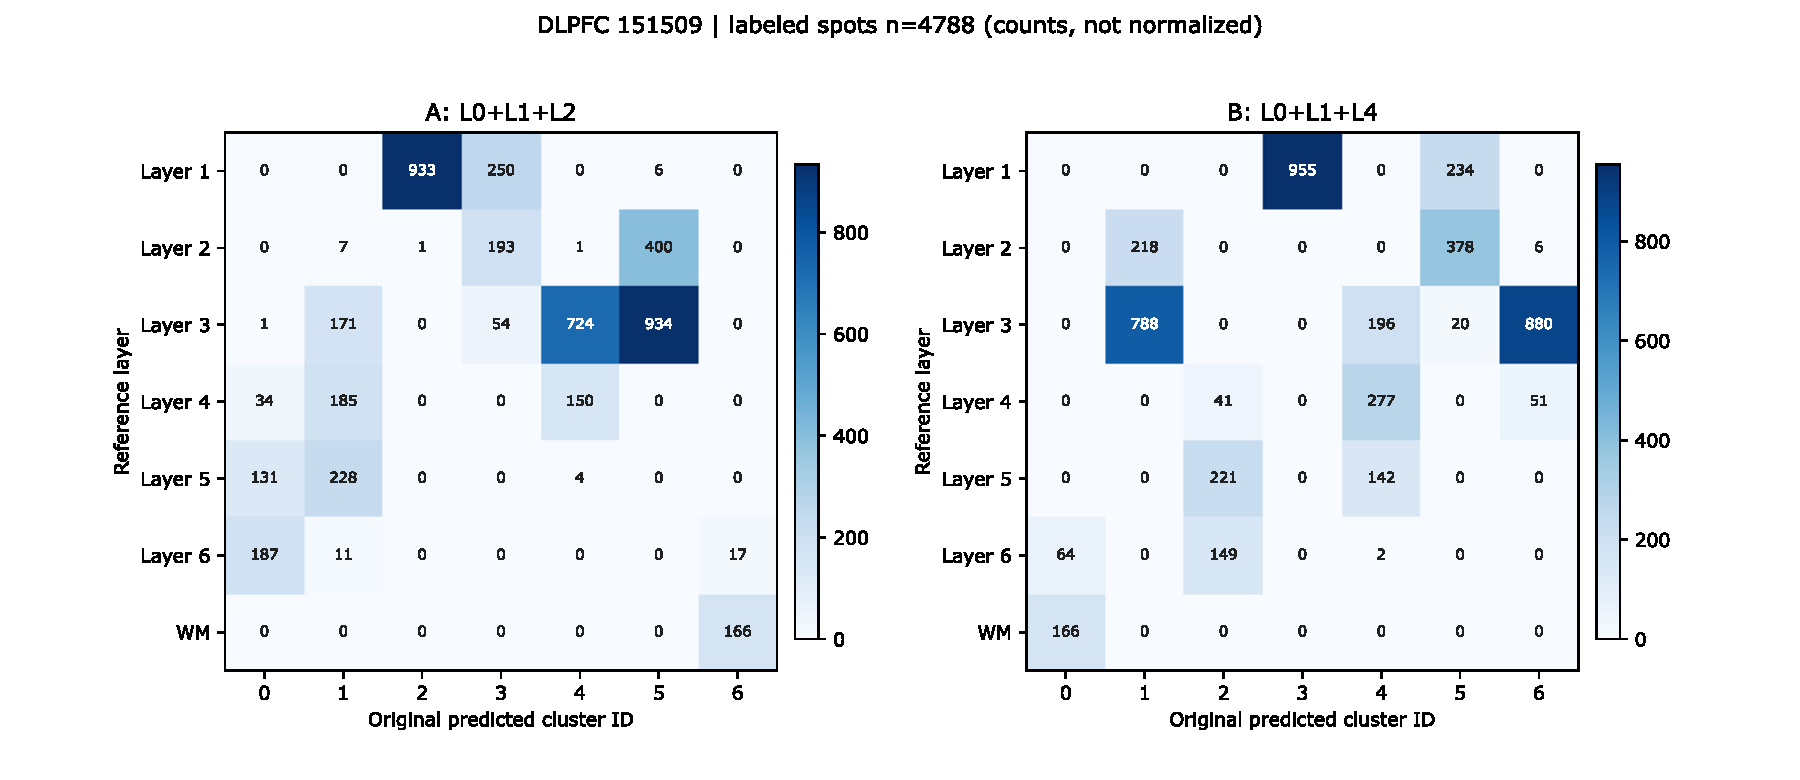
\includegraphics[width=0.97\linewidth,height=0.72\textheight,keepaspectratio]{E4_SOURCE_FIGURES_20261122_RELEASE/figures_pdf/151509/151509_reference_A_B_confusion.pdf}
\captionof{figure}{DLPFC切片151509：参考层与A/B簇交叉计数图（原始E4图件转换的矢量PDF；聚类编号未根据参考标签重排）。}
\label{fig:cc-e4-app-151509-confusion}
\end{minipage}\par\medskip
}{%
\par\noindent\emph{[待插入原始E4图件：151509_reference_A_B_confusion.svg]}\par
}
\subsection{DLPFC切片151510}
\IfFileExists{E4_SOURCE_FIGURES_20261122_RELEASE/figures_pdf/151510/151510_reference_A_B_spatial.pdf}{%
\par\noindent\begin{minipage}{\linewidth}
\centering
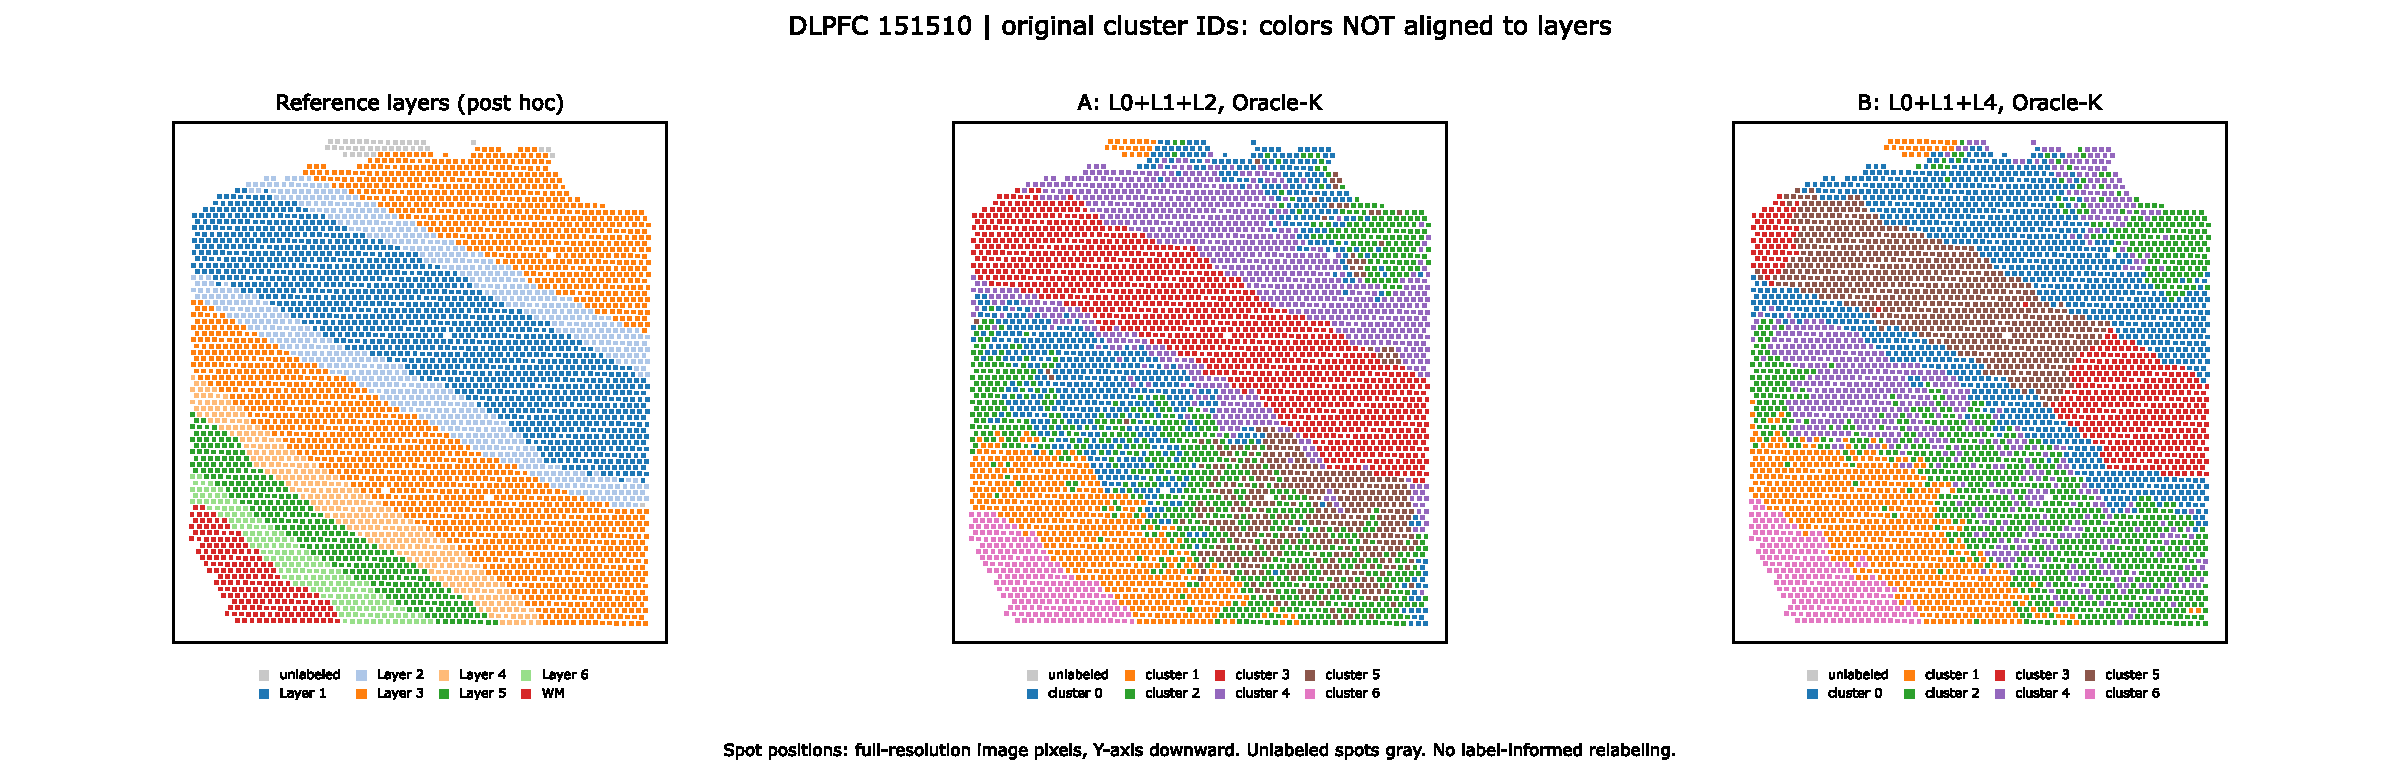
\includegraphics[width=0.97\linewidth,height=0.72\textheight,keepaspectratio]{E4_SOURCE_FIGURES_20261122_RELEASE/figures_pdf/151510/151510_reference_A_B_spatial.pdf}
\captionof{figure}{DLPFC切片151510：参考层与A/B原始聚类三联图（原始E4图件转换的矢量PDF；聚类编号未根据参考标签重排）。}
\label{fig:cc-e4-app-151510-map}
\end{minipage}\par\medskip
}{%
\par\noindent\emph{[待插入原始E4图件：151510_reference_A_B_spatial.svg]}\par
}
\IfFileExists{E4_SOURCE_FIGURES_20261122_RELEASE/figures_pdf/151510/151510_MOBP_PCP4_SNAP25_expression.pdf}{%
\par\noindent\begin{minipage}{\linewidth}
\centering
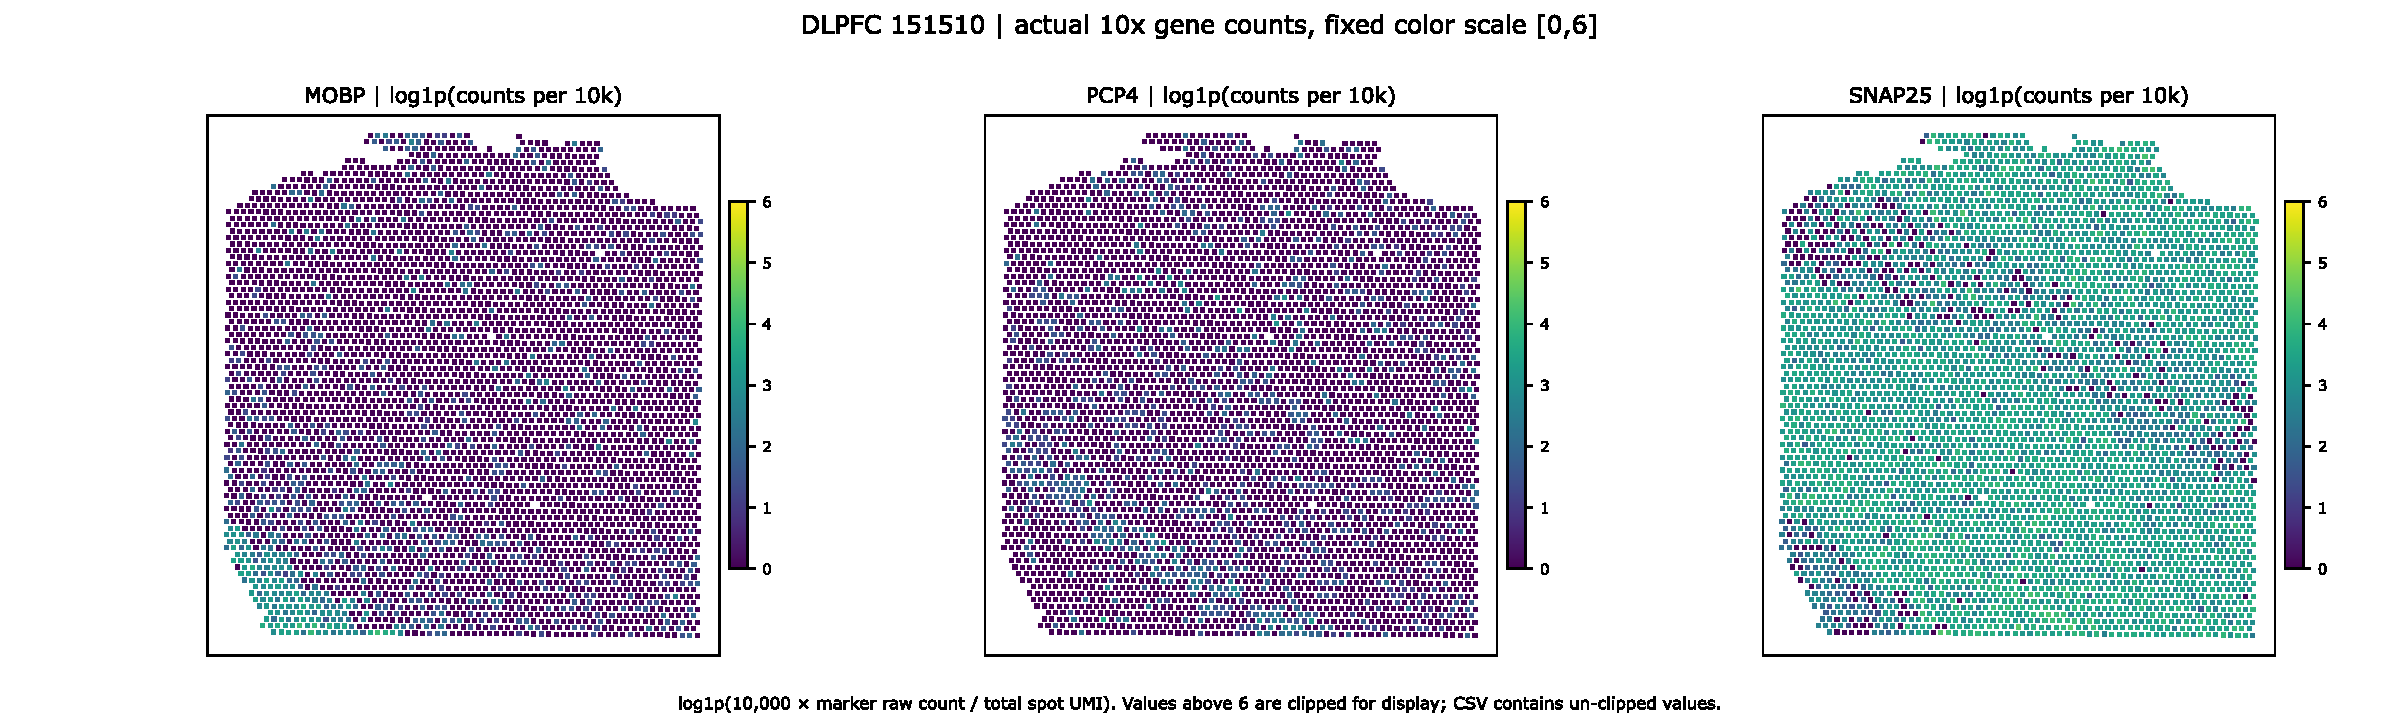
\includegraphics[width=0.97\linewidth,height=0.72\textheight,keepaspectratio]{E4_SOURCE_FIGURES_20261122_RELEASE/figures_pdf/151510/151510_MOBP_PCP4_SNAP25_expression.pdf}
\captionof{figure}{DLPFC切片151510：MOBP/PCP4/SNAP25表达三联图（原始E4图件转换的矢量PDF；聚类编号未根据参考标签重排）。}
\label{fig:cc-e4-app-151510-markers}
\end{minipage}\par\medskip
}{%
\par\noindent\emph{[待插入原始E4图件：151510_MOBP_PCP4_SNAP25_expression.svg]}\par
}
\IfFileExists{E4_SOURCE_FIGURES_20261122_RELEASE/figures_pdf/151510/151510_reference_A_B_confusion.pdf}{%
\par\noindent\begin{minipage}{\linewidth}
\centering
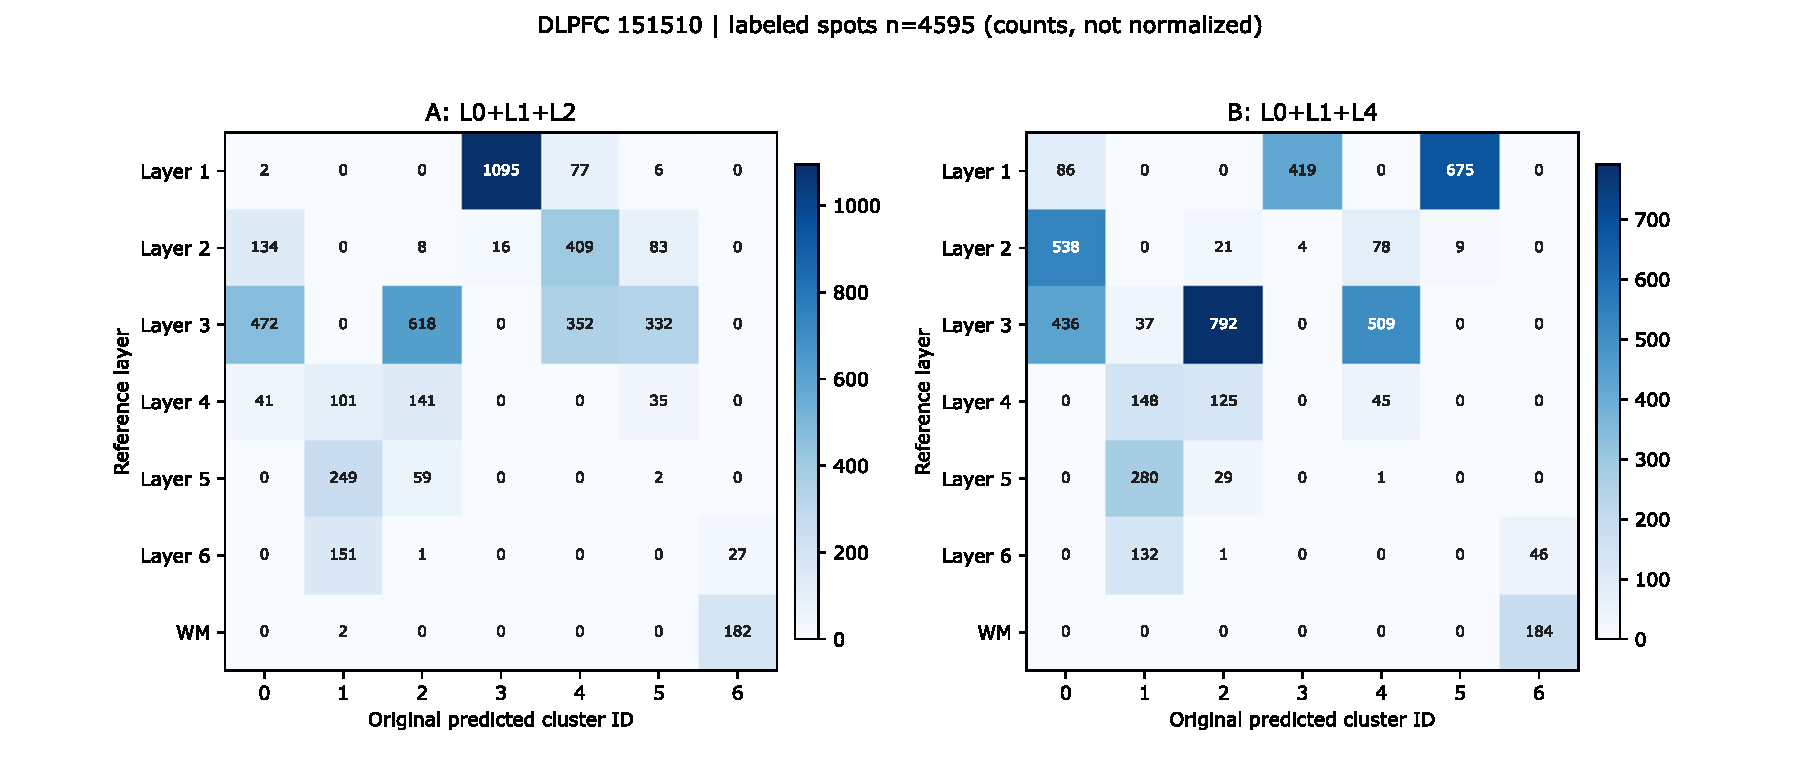
\includegraphics[width=0.97\linewidth,height=0.72\textheight,keepaspectratio]{E4_SOURCE_FIGURES_20261122_RELEASE/figures_pdf/151510/151510_reference_A_B_confusion.pdf}
\captionof{figure}{DLPFC切片151510：参考层与A/B簇交叉计数图（原始E4图件转换的矢量PDF；聚类编号未根据参考标签重排）。}
\label{fig:cc-e4-app-151510-confusion}
\end{minipage}\par\medskip
}{%
\par\noindent\emph{[待插入原始E4图件：151510_reference_A_B_confusion.svg]}\par
}
\subsection{DLPFC切片151669}
\IfFileExists{E4_SOURCE_FIGURES_20261122_RELEASE/figures_pdf/151669/151669_reference_A_B_spatial.pdf}{%
\par\noindent\begin{minipage}{\linewidth}
\centering
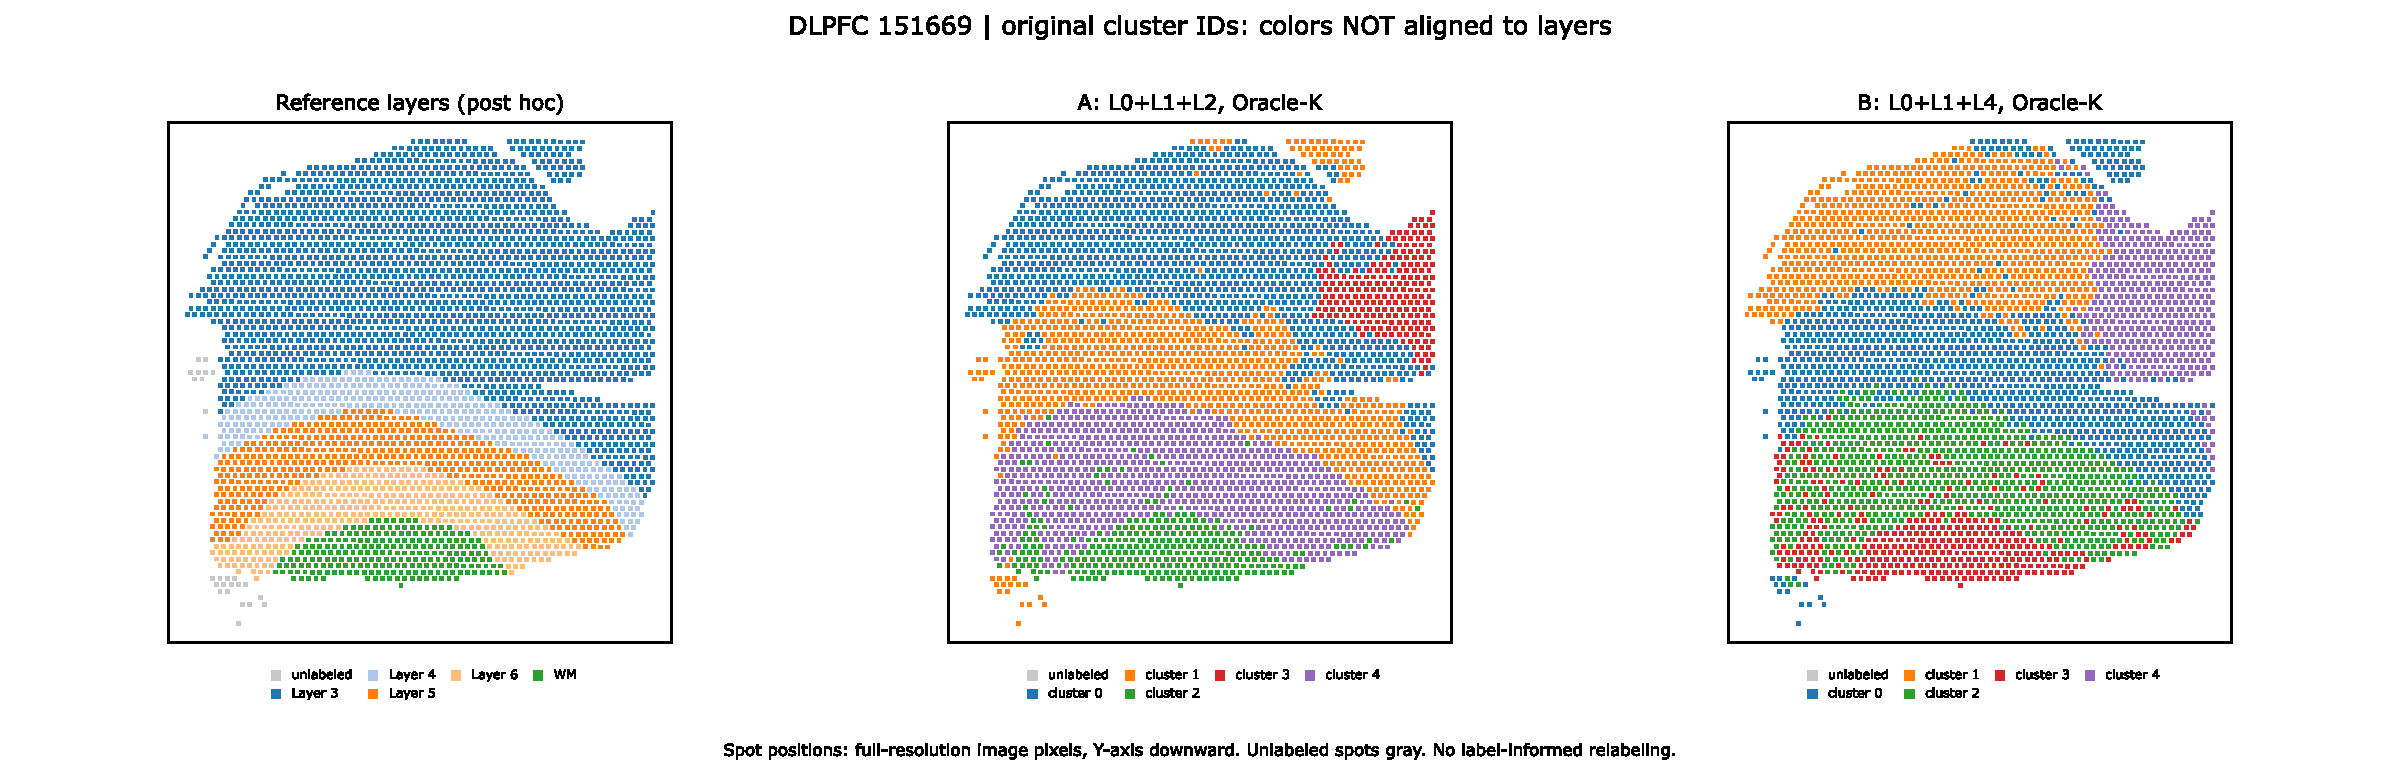
\includegraphics[width=0.97\linewidth,height=0.72\textheight,keepaspectratio]{E4_SOURCE_FIGURES_20261122_RELEASE/figures_pdf/151669/151669_reference_A_B_spatial.pdf}
\captionof{figure}{DLPFC切片151669：参考层与A/B原始聚类三联图（原始E4图件转换的矢量PDF；聚类编号未根据参考标签重排）。}
\label{fig:cc-e4-app-151669-map}
\end{minipage}\par\medskip
}{%
\par\noindent\emph{[待插入原始E4图件：151669_reference_A_B_spatial.svg]}\par
}
\IfFileExists{E4_SOURCE_FIGURES_20261122_RELEASE/figures_pdf/151669/151669_MOBP_PCP4_SNAP25_expression.pdf}{%
\par\noindent\begin{minipage}{\linewidth}
\centering
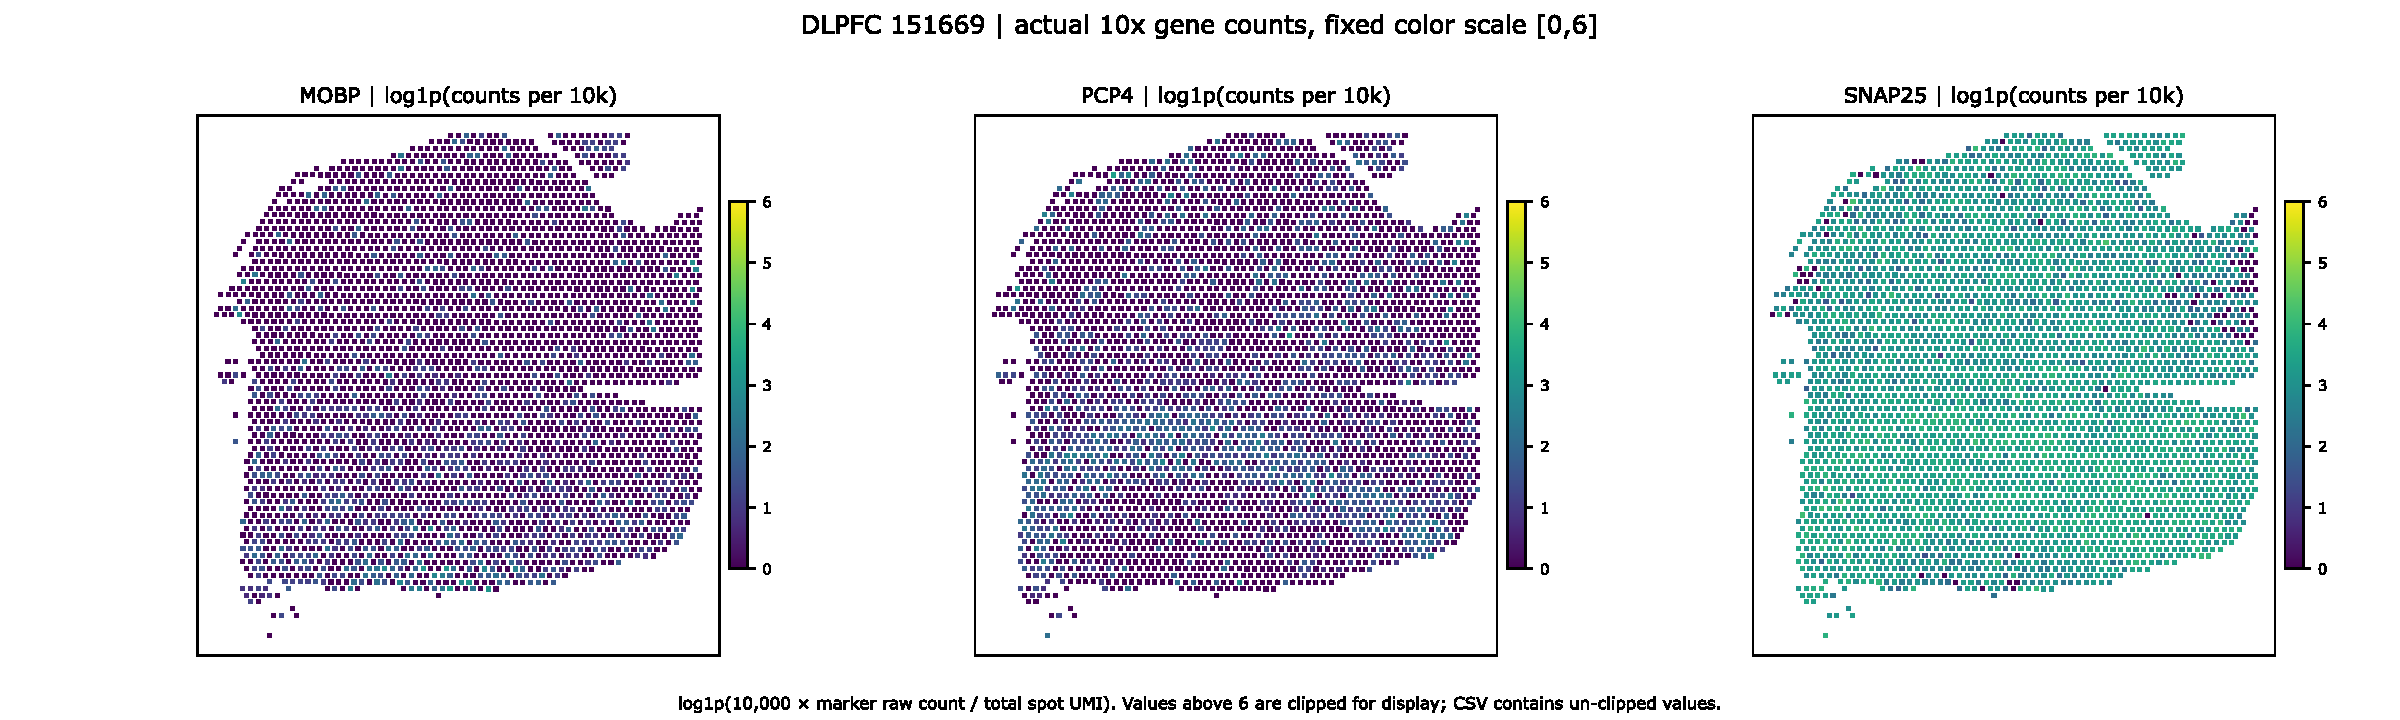
\includegraphics[width=0.97\linewidth,height=0.72\textheight,keepaspectratio]{E4_SOURCE_FIGURES_20261122_RELEASE/figures_pdf/151669/151669_MOBP_PCP4_SNAP25_expression.pdf}
\captionof{figure}{DLPFC切片151669：MOBP/PCP4/SNAP25表达三联图（原始E4图件转换的矢量PDF；聚类编号未根据参考标签重排）。}
\label{fig:cc-e4-app-151669-markers}
\end{minipage}\par\medskip
}{%
\par\noindent\emph{[待插入原始E4图件：151669_MOBP_PCP4_SNAP25_expression.svg]}\par
}
\IfFileExists{E4_SOURCE_FIGURES_20261122_RELEASE/figures_pdf/151669/151669_reference_A_B_confusion.pdf}{%
\par\noindent\begin{minipage}{\linewidth}
\centering
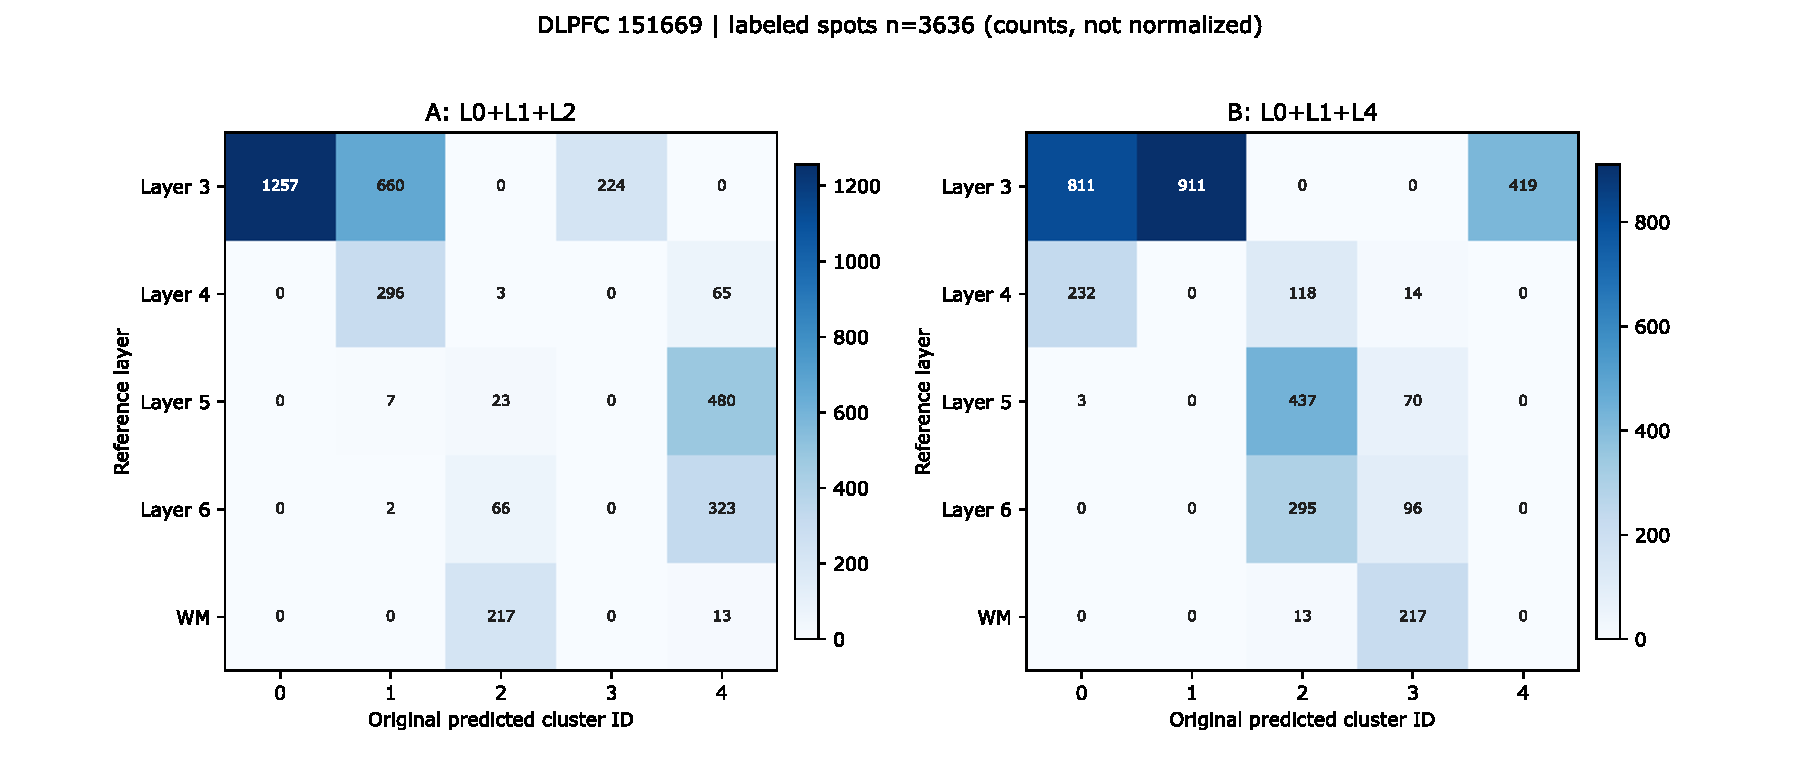
\includegraphics[width=0.97\linewidth,height=0.72\textheight,keepaspectratio]{E4_SOURCE_FIGURES_20261122_RELEASE/figures_pdf/151669/151669_reference_A_B_confusion.pdf}
\captionof{figure}{DLPFC切片151669：参考层与A/B簇交叉计数图（原始E4图件转换的矢量PDF；聚类编号未根据参考标签重排）。}
\label{fig:cc-e4-app-151669-confusion}
\end{minipage}\par\medskip
}{%
\par\noindent\emph{[待插入原始E4图件：151669_reference_A_B_confusion.svg]}\par
}
\subsection{DLPFC切片151670}
\IfFileExists{E4_SOURCE_FIGURES_20261122_RELEASE/figures_pdf/151670/151670_reference_A_B_spatial.pdf}{%
\par\noindent\begin{minipage}{\linewidth}
\centering
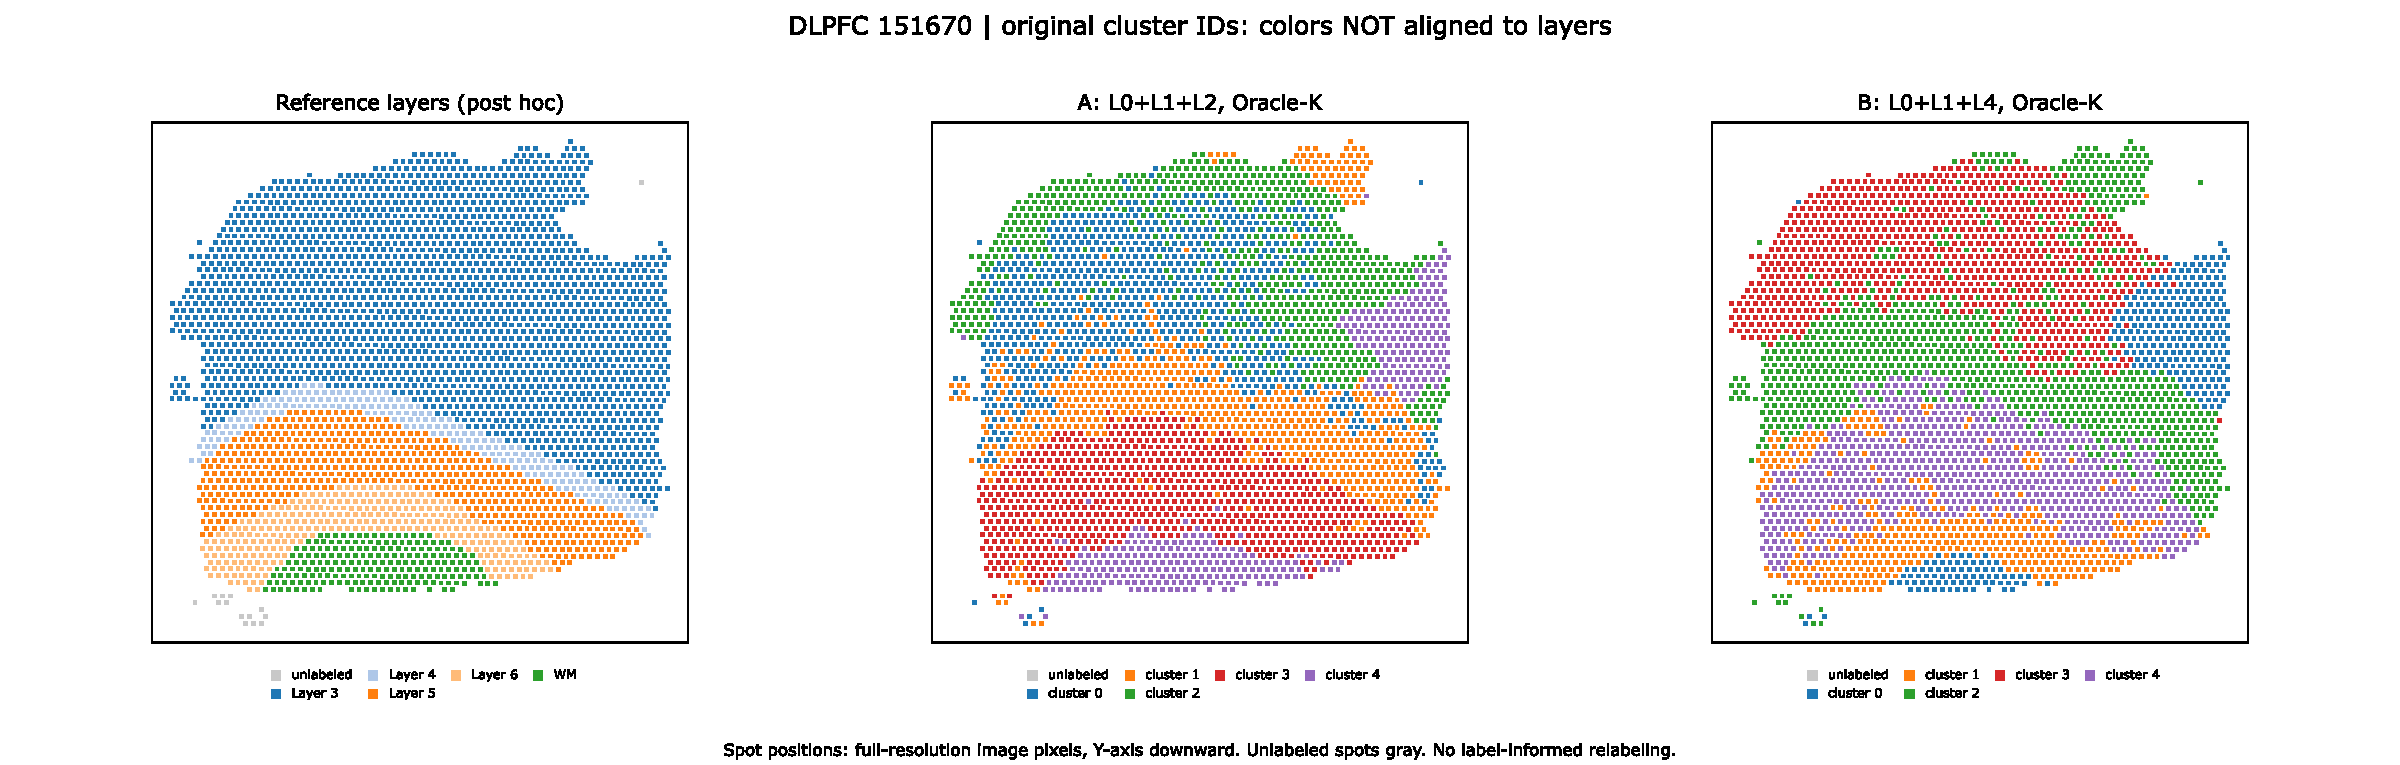
\includegraphics[width=0.97\linewidth,height=0.72\textheight,keepaspectratio]{E4_SOURCE_FIGURES_20261122_RELEASE/figures_pdf/151670/151670_reference_A_B_spatial.pdf}
\captionof{figure}{DLPFC切片151670：参考层与A/B原始聚类三联图（原始E4图件转换的矢量PDF；聚类编号未根据参考标签重排）。}
\label{fig:cc-e4-app-151670-map}
\end{minipage}\par\medskip
}{%
\par\noindent\emph{[待插入原始E4图件：151670_reference_A_B_spatial.svg]}\par
}
\IfFileExists{E4_SOURCE_FIGURES_20261122_RELEASE/figures_pdf/151670/151670_MOBP_PCP4_SNAP25_expression.pdf}{%
\par\noindent\begin{minipage}{\linewidth}
\centering
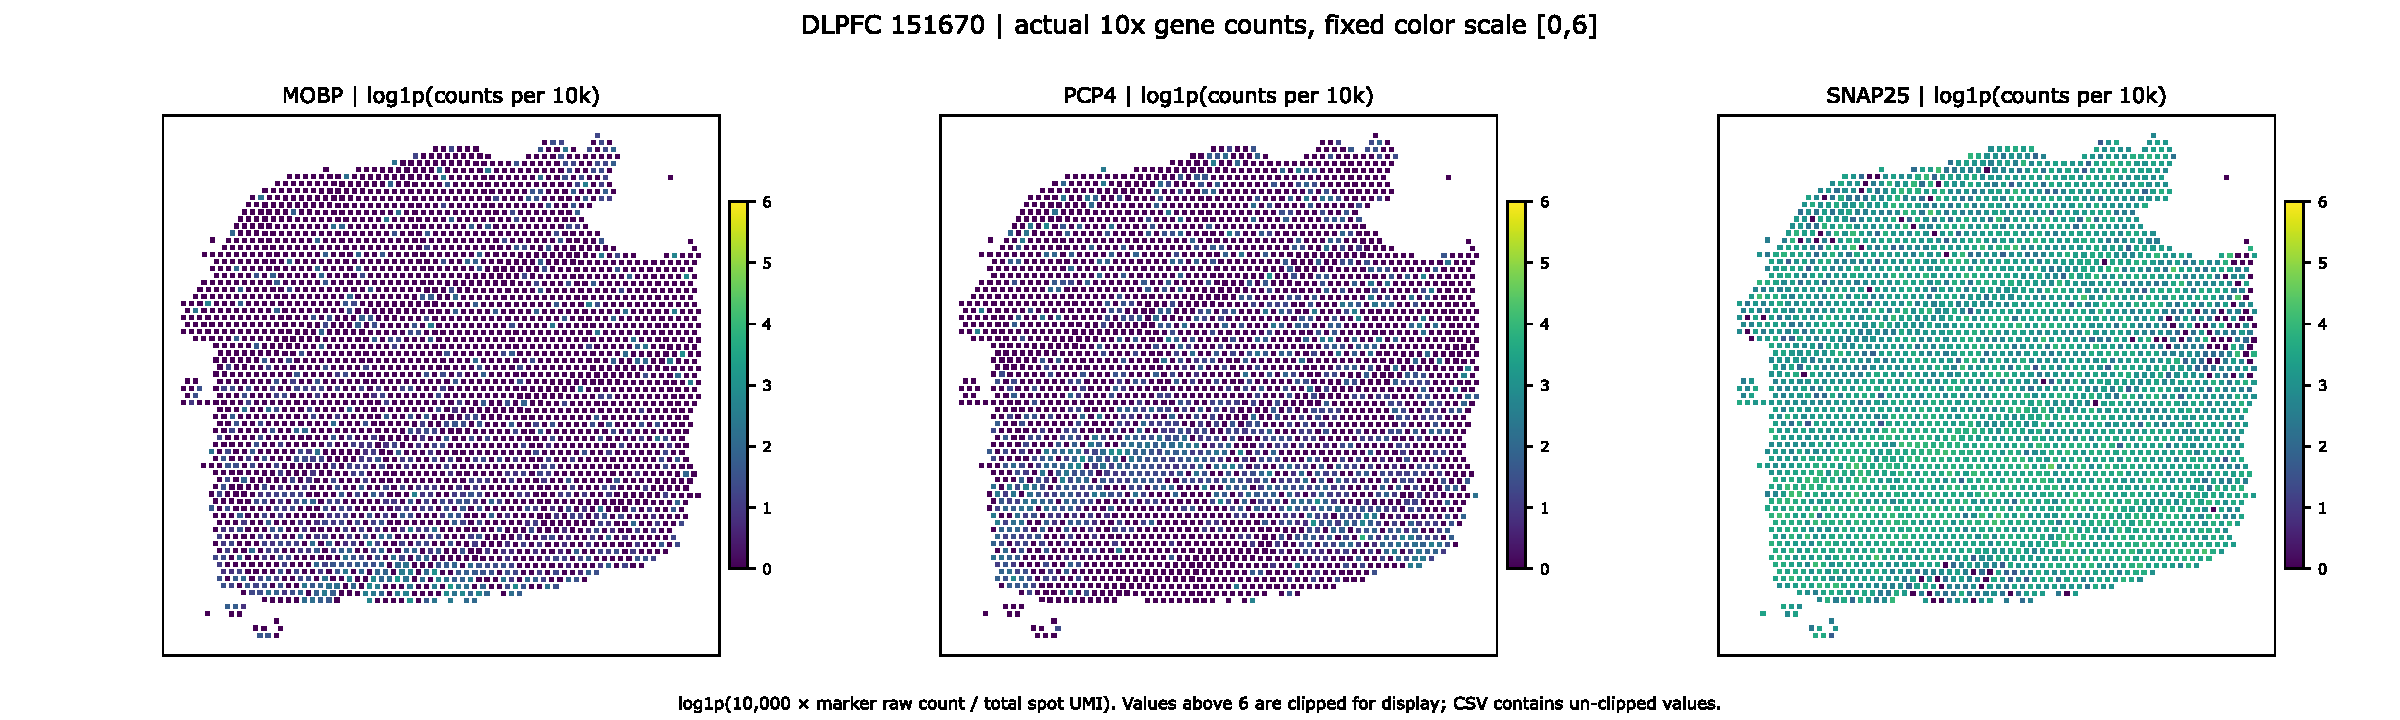
\includegraphics[width=0.97\linewidth,height=0.72\textheight,keepaspectratio]{E4_SOURCE_FIGURES_20261122_RELEASE/figures_pdf/151670/151670_MOBP_PCP4_SNAP25_expression.pdf}
\captionof{figure}{DLPFC切片151670：MOBP/PCP4/SNAP25表达三联图（原始E4图件转换的矢量PDF；聚类编号未根据参考标签重排）。}
\label{fig:cc-e4-app-151670-markers}
\end{minipage}\par\medskip
}{%
\par\noindent\emph{[待插入原始E4图件：151670_MOBP_PCP4_SNAP25_expression.svg]}\par
}
\IfFileExists{E4_SOURCE_FIGURES_20261122_RELEASE/figures_pdf/151670/151670_reference_A_B_confusion.pdf}{%
\par\noindent\begin{minipage}{\linewidth}
\centering
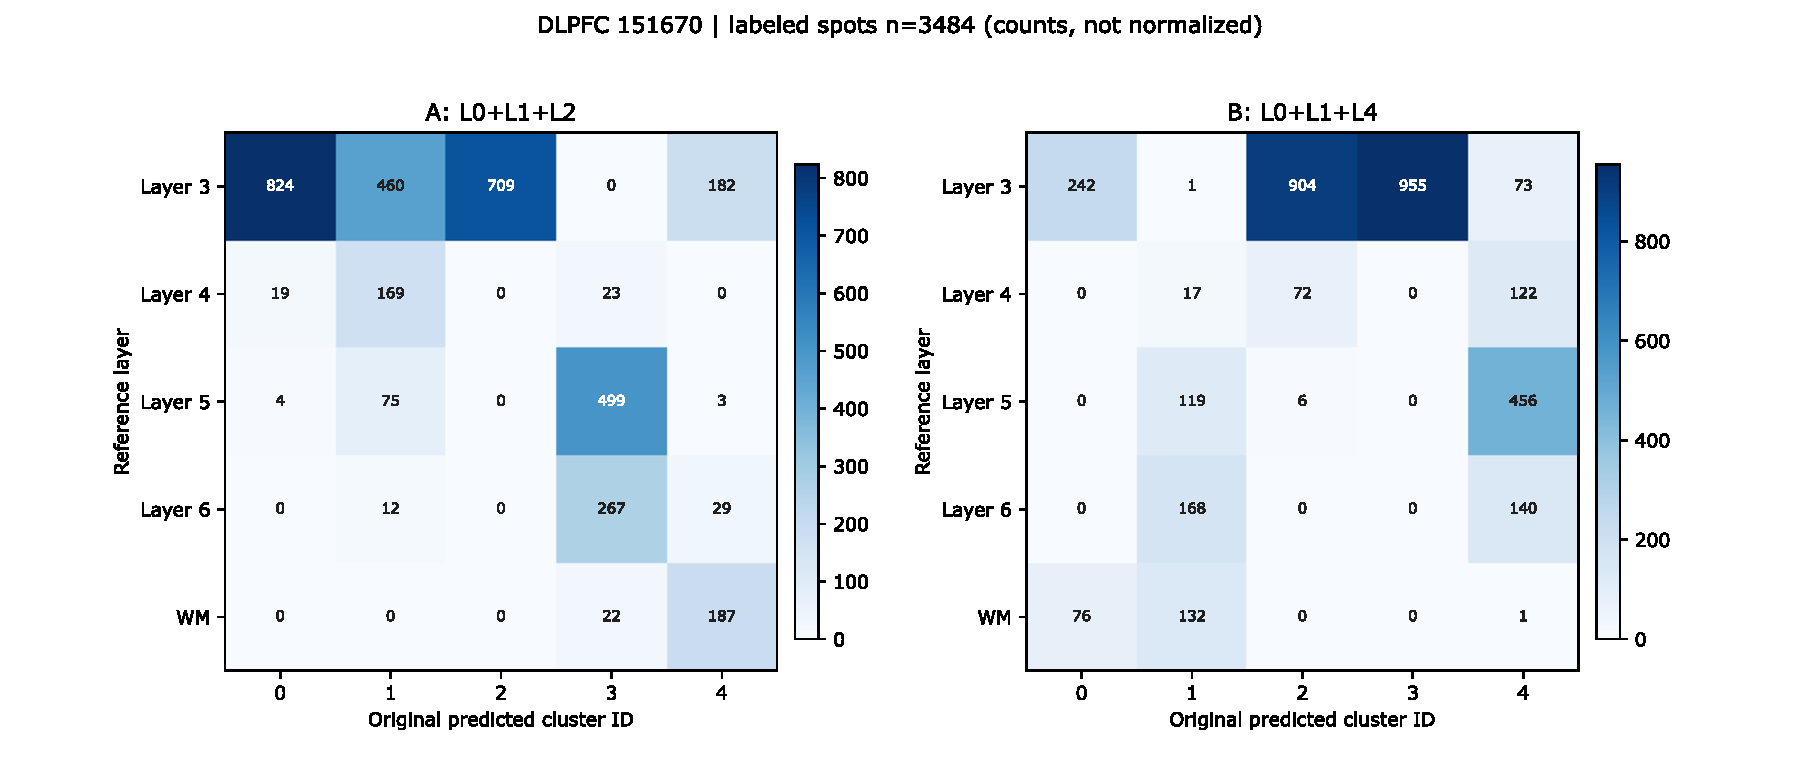
\includegraphics[width=0.97\linewidth,height=0.72\textheight,keepaspectratio]{E4_SOURCE_FIGURES_20261122_RELEASE/figures_pdf/151670/151670_reference_A_B_confusion.pdf}
\captionof{figure}{DLPFC切片151670：参考层与A/B簇交叉计数图（原始E4图件转换的矢量PDF；聚类编号未根据参考标签重排）。}
\label{fig:cc-e4-app-151670-confusion}
\end{minipage}\par\medskip
}{%
\par\noindent\emph{[待插入原始E4图件：151670_reference_A_B_confusion.svg]}\par
}
\subsection{DLPFC切片151671}
\IfFileExists{E4_SOURCE_FIGURES_20261122_RELEASE/figures_pdf/151671/151671_reference_A_B_spatial.pdf}{%
\par\noindent\begin{minipage}{\linewidth}
\centering
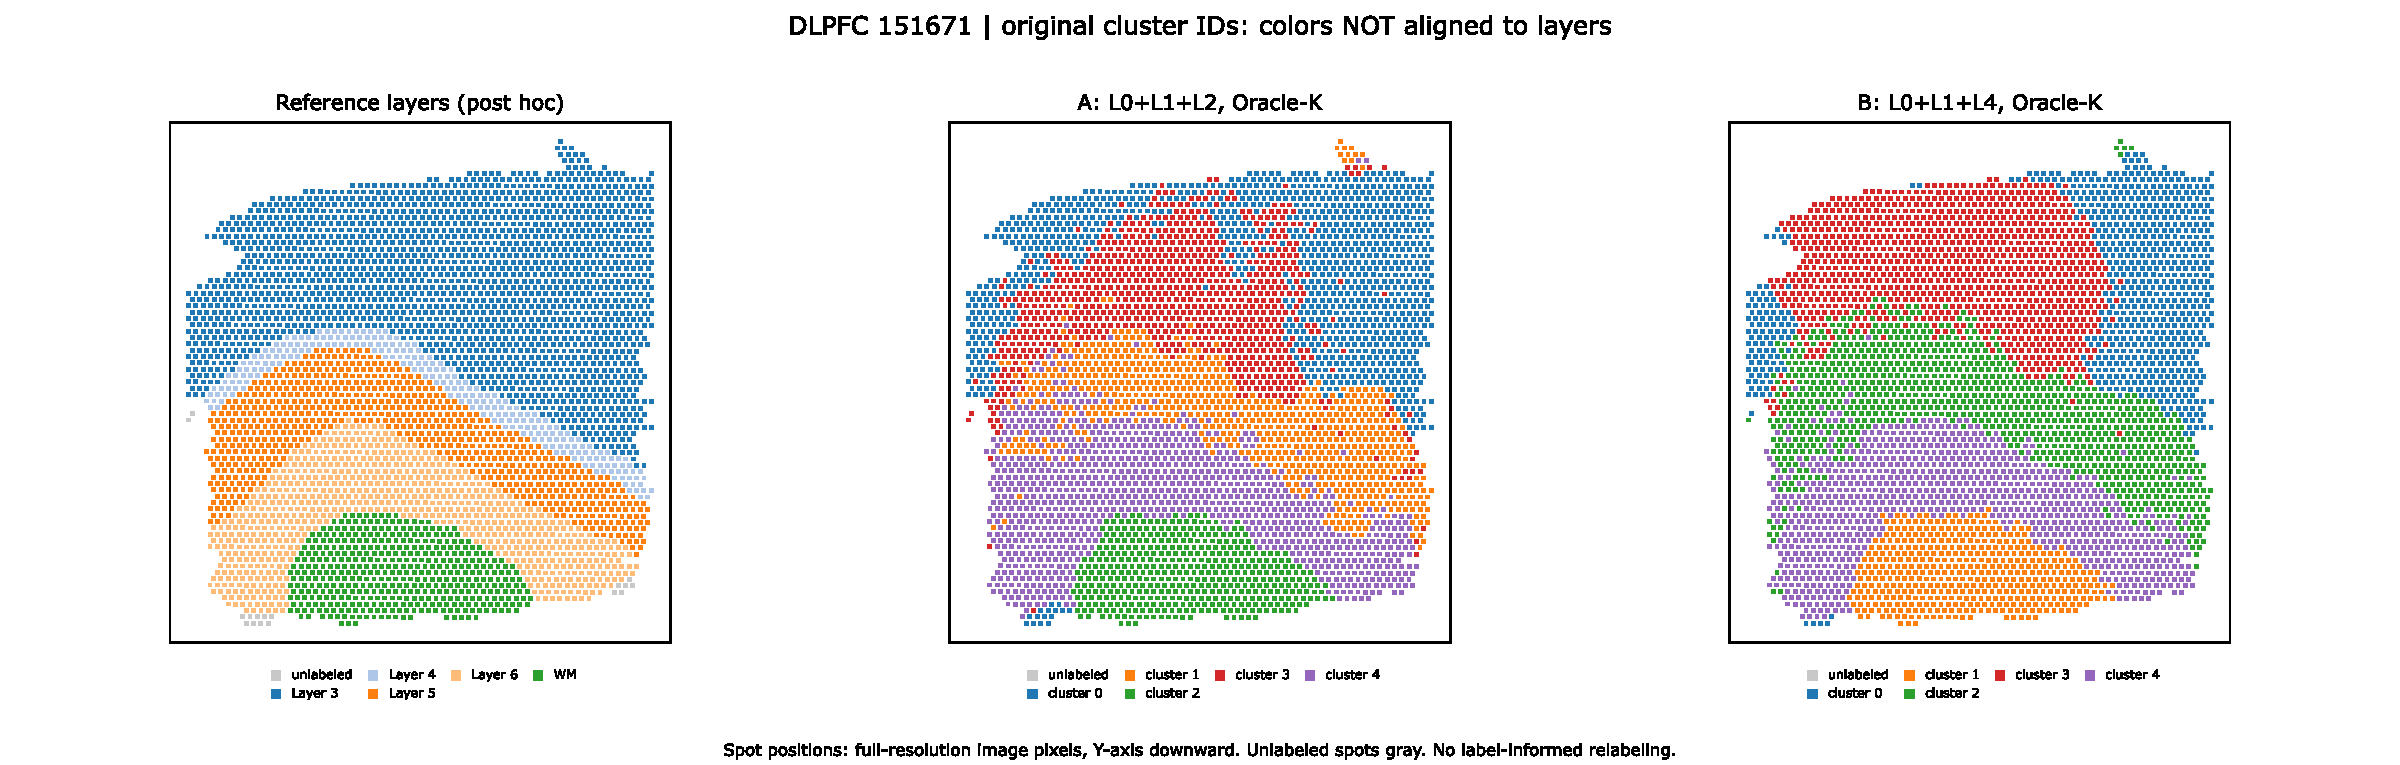
\includegraphics[width=0.97\linewidth,height=0.72\textheight,keepaspectratio]{E4_SOURCE_FIGURES_20261122_RELEASE/figures_pdf/151671/151671_reference_A_B_spatial.pdf}
\captionof{figure}{DLPFC切片151671：参考层与A/B原始聚类三联图（原始E4图件转换的矢量PDF；聚类编号未根据参考标签重排）。}
\label{fig:cc-e4-app-151671-map}
\end{minipage}\par\medskip
}{%
\par\noindent\emph{[待插入原始E4图件：151671_reference_A_B_spatial.svg]}\par
}
\IfFileExists{E4_SOURCE_FIGURES_20261122_RELEASE/figures_pdf/151671/151671_MOBP_PCP4_SNAP25_expression.pdf}{%
\par\noindent\begin{minipage}{\linewidth}
\centering
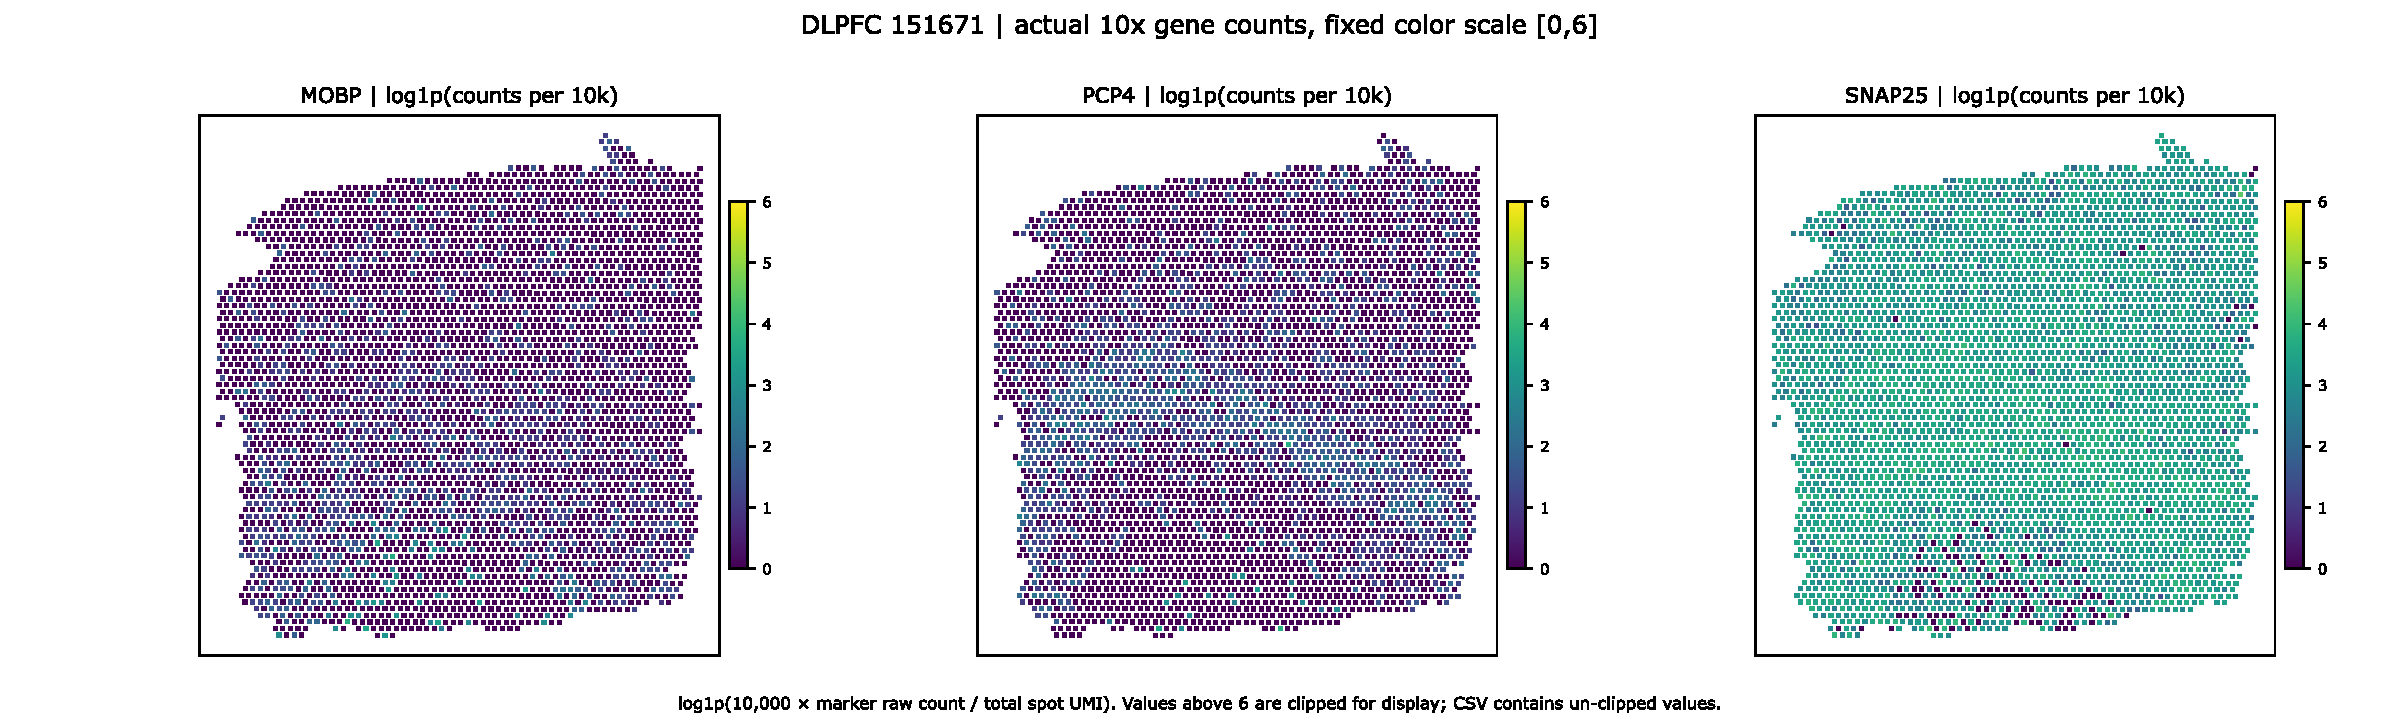
\includegraphics[width=0.97\linewidth,height=0.72\textheight,keepaspectratio]{E4_SOURCE_FIGURES_20261122_RELEASE/figures_pdf/151671/151671_MOBP_PCP4_SNAP25_expression.pdf}
\captionof{figure}{DLPFC切片151671：MOBP/PCP4/SNAP25表达三联图（原始E4图件转换的矢量PDF；聚类编号未根据参考标签重排）。}
\label{fig:cc-e4-app-151671-markers}
\end{minipage}\par\medskip
}{%
\par\noindent\emph{[待插入原始E4图件：151671_MOBP_PCP4_SNAP25_expression.svg]}\par
}
\IfFileExists{E4_SOURCE_FIGURES_20261122_RELEASE/figures_pdf/151671/151671_reference_A_B_confusion.pdf}{%
\par\noindent\begin{minipage}{\linewidth}
\centering
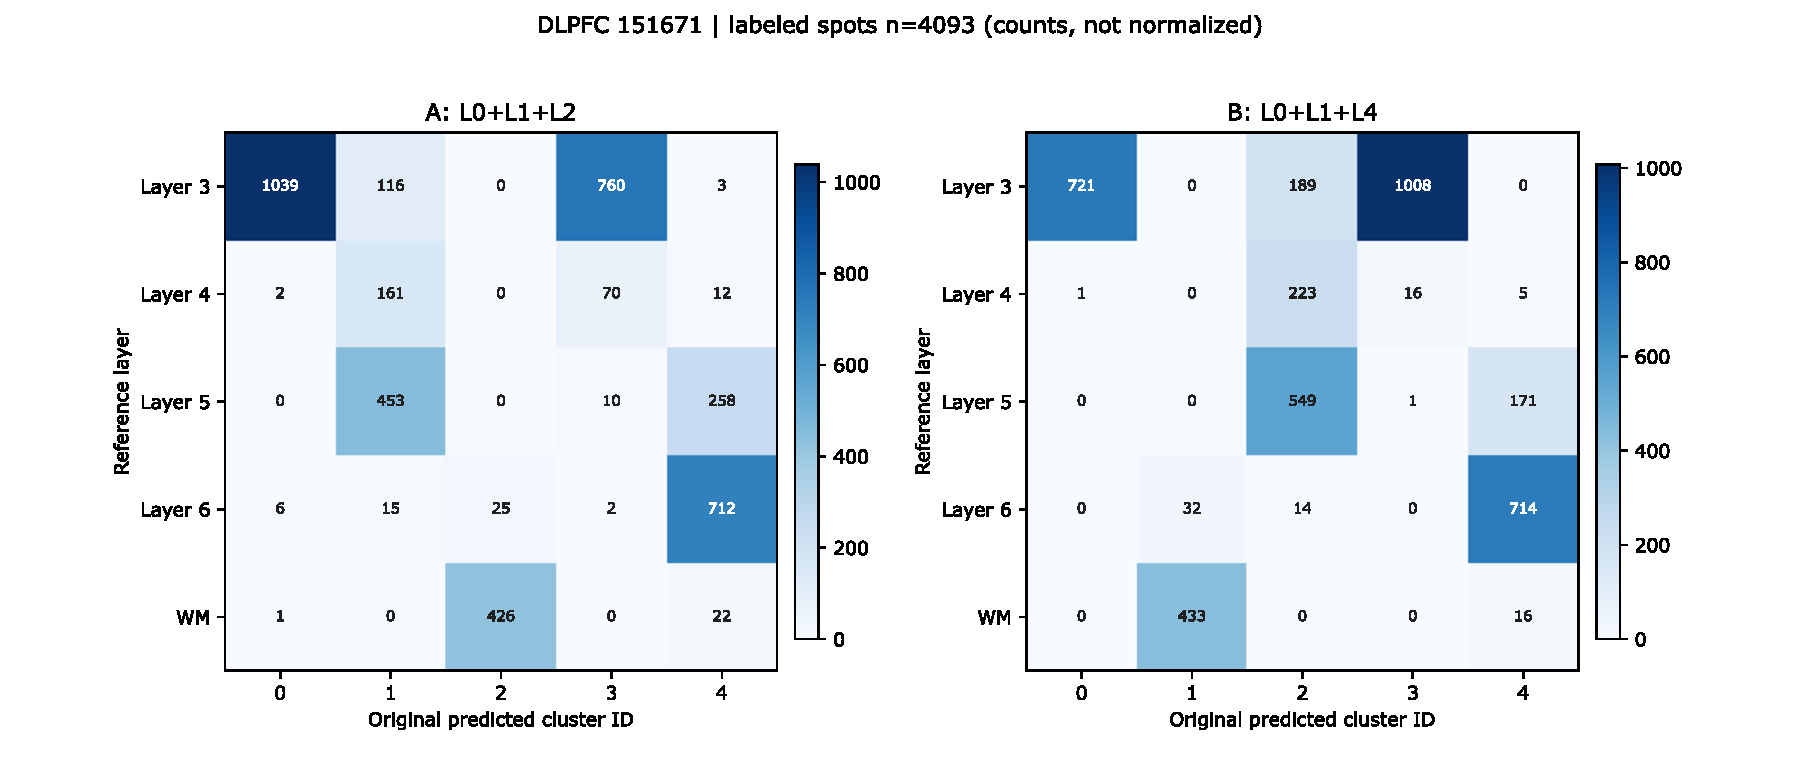
\includegraphics[width=0.97\linewidth,height=0.72\textheight,keepaspectratio]{E4_SOURCE_FIGURES_20261122_RELEASE/figures_pdf/151671/151671_reference_A_B_confusion.pdf}
\captionof{figure}{DLPFC切片151671：参考层与A/B簇交叉计数图（原始E4图件转换的矢量PDF；聚类编号未根据参考标签重排）。}
\label{fig:cc-e4-app-151671-confusion}
\end{minipage}\par\medskip
}{%
\par\noindent\emph{[待插入原始E4图件：151671_reference_A_B_confusion.svg]}\par
}
\subsection{DLPFC切片151672}
\IfFileExists{E4_SOURCE_FIGURES_20261122_RELEASE/figures_pdf/151672/151672_reference_A_B_spatial.pdf}{%
\par\noindent\begin{minipage}{\linewidth}
\centering
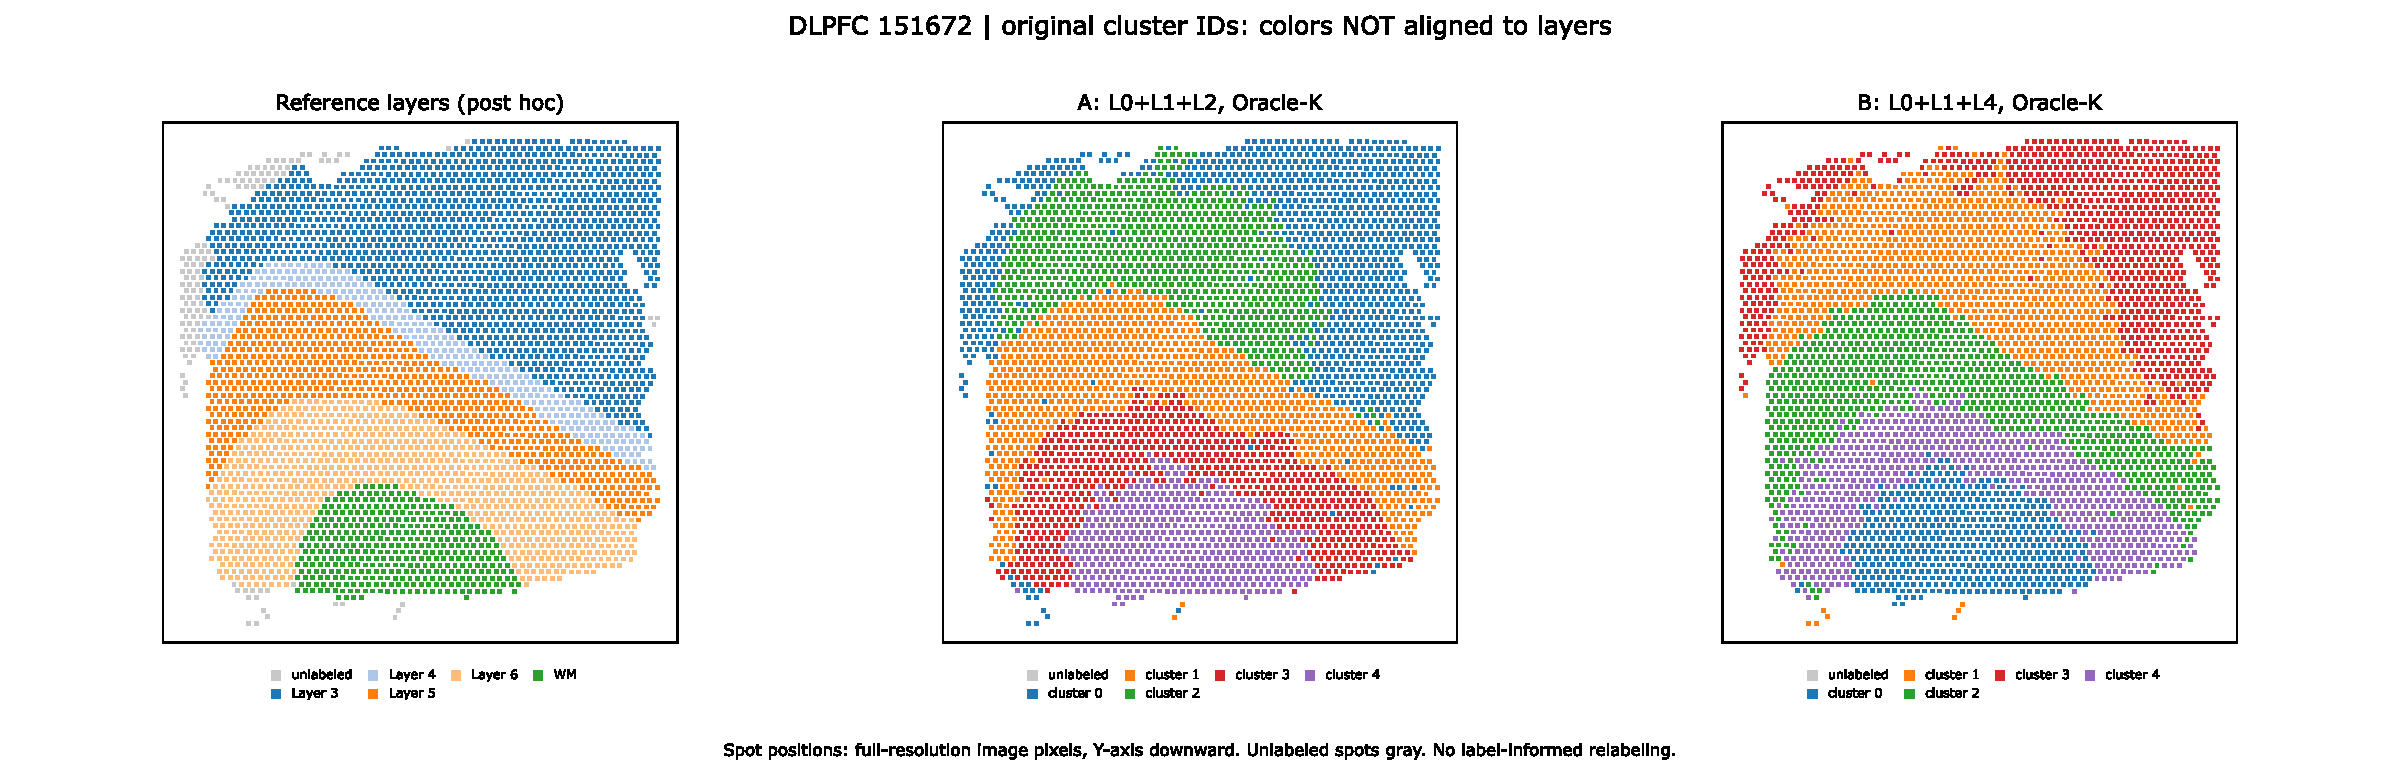
\includegraphics[width=0.97\linewidth,height=0.72\textheight,keepaspectratio]{E4_SOURCE_FIGURES_20261122_RELEASE/figures_pdf/151672/151672_reference_A_B_spatial.pdf}
\captionof{figure}{DLPFC切片151672：参考层与A/B原始聚类三联图（原始E4图件转换的矢量PDF；聚类编号未根据参考标签重排）。}
\label{fig:cc-e4-app-151672-map}
\end{minipage}\par\medskip
}{%
\par\noindent\emph{[待插入原始E4图件：151672_reference_A_B_spatial.svg]}\par
}
\IfFileExists{E4_SOURCE_FIGURES_20261122_RELEASE/figures_pdf/151672/151672_MOBP_PCP4_SNAP25_expression.pdf}{%
\par\noindent\begin{minipage}{\linewidth}
\centering
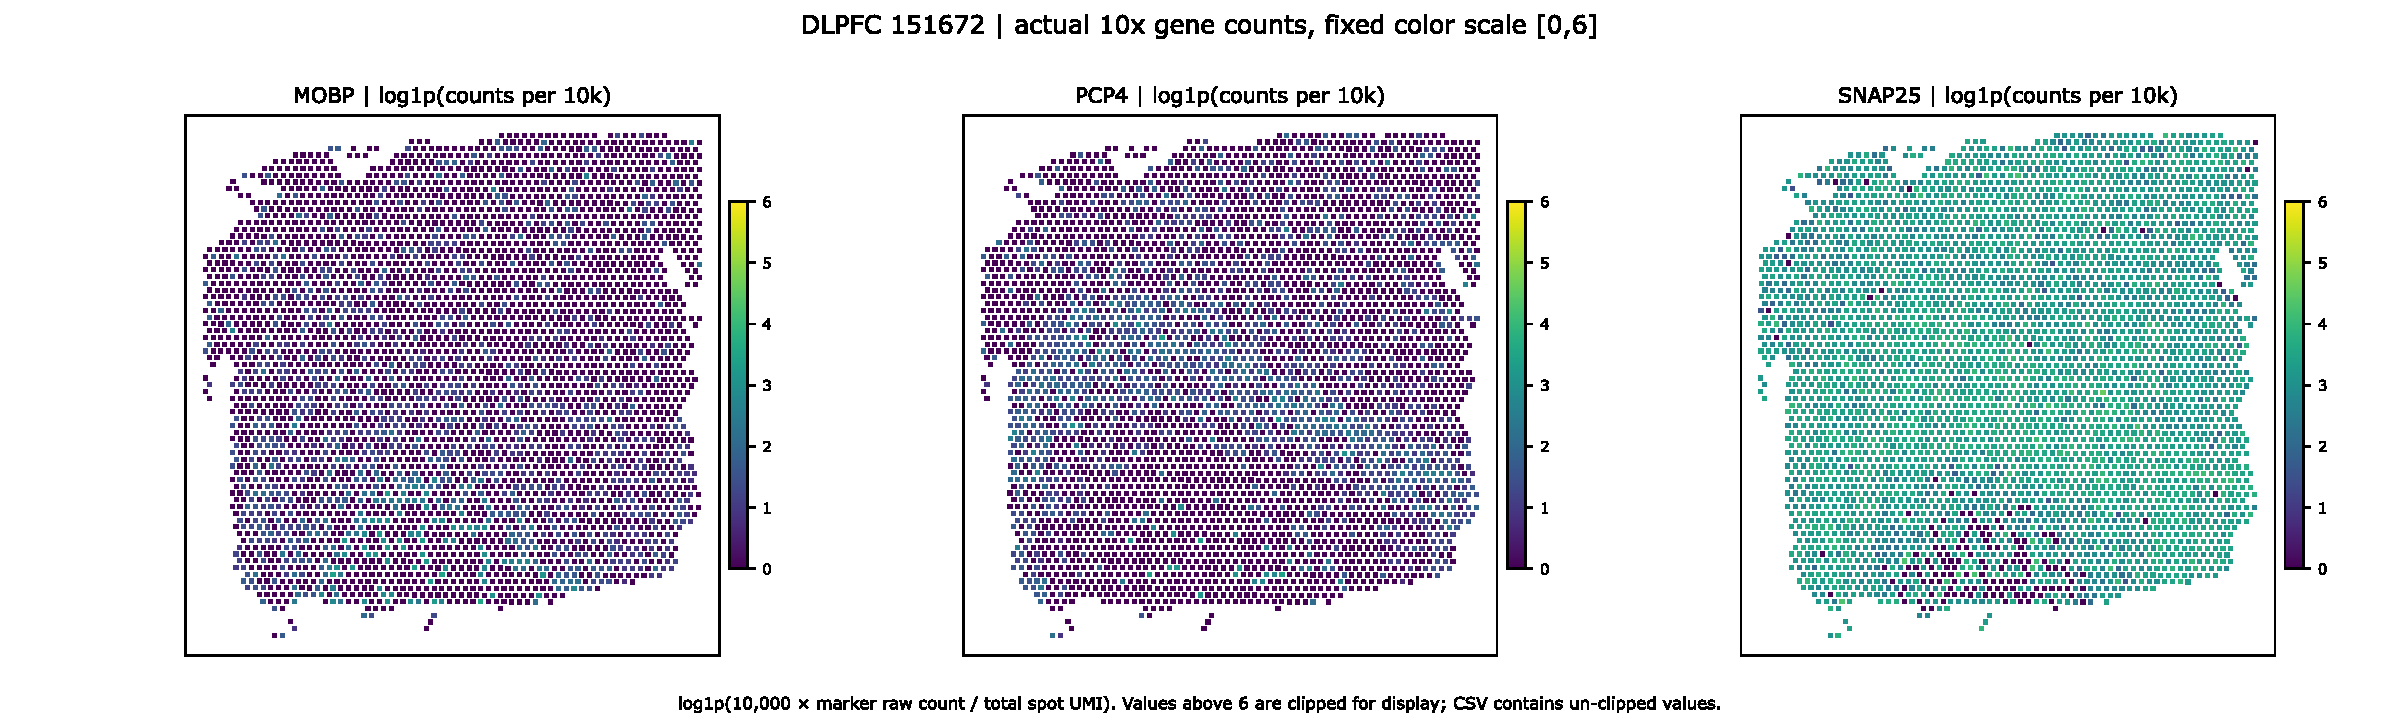
\includegraphics[width=0.97\linewidth,height=0.72\textheight,keepaspectratio]{E4_SOURCE_FIGURES_20261122_RELEASE/figures_pdf/151672/151672_MOBP_PCP4_SNAP25_expression.pdf}
\captionof{figure}{DLPFC切片151672：MOBP/PCP4/SNAP25表达三联图（原始E4图件转换的矢量PDF；聚类编号未根据参考标签重排）。}
\label{fig:cc-e4-app-151672-markers}
\end{minipage}\par\medskip
}{%
\par\noindent\emph{[待插入原始E4图件：151672_MOBP_PCP4_SNAP25_expression.svg]}\par
}
\IfFileExists{E4_SOURCE_FIGURES_20261122_RELEASE/figures_pdf/151672/151672_reference_A_B_confusion.pdf}{%
\par\noindent\begin{minipage}{\linewidth}
\centering
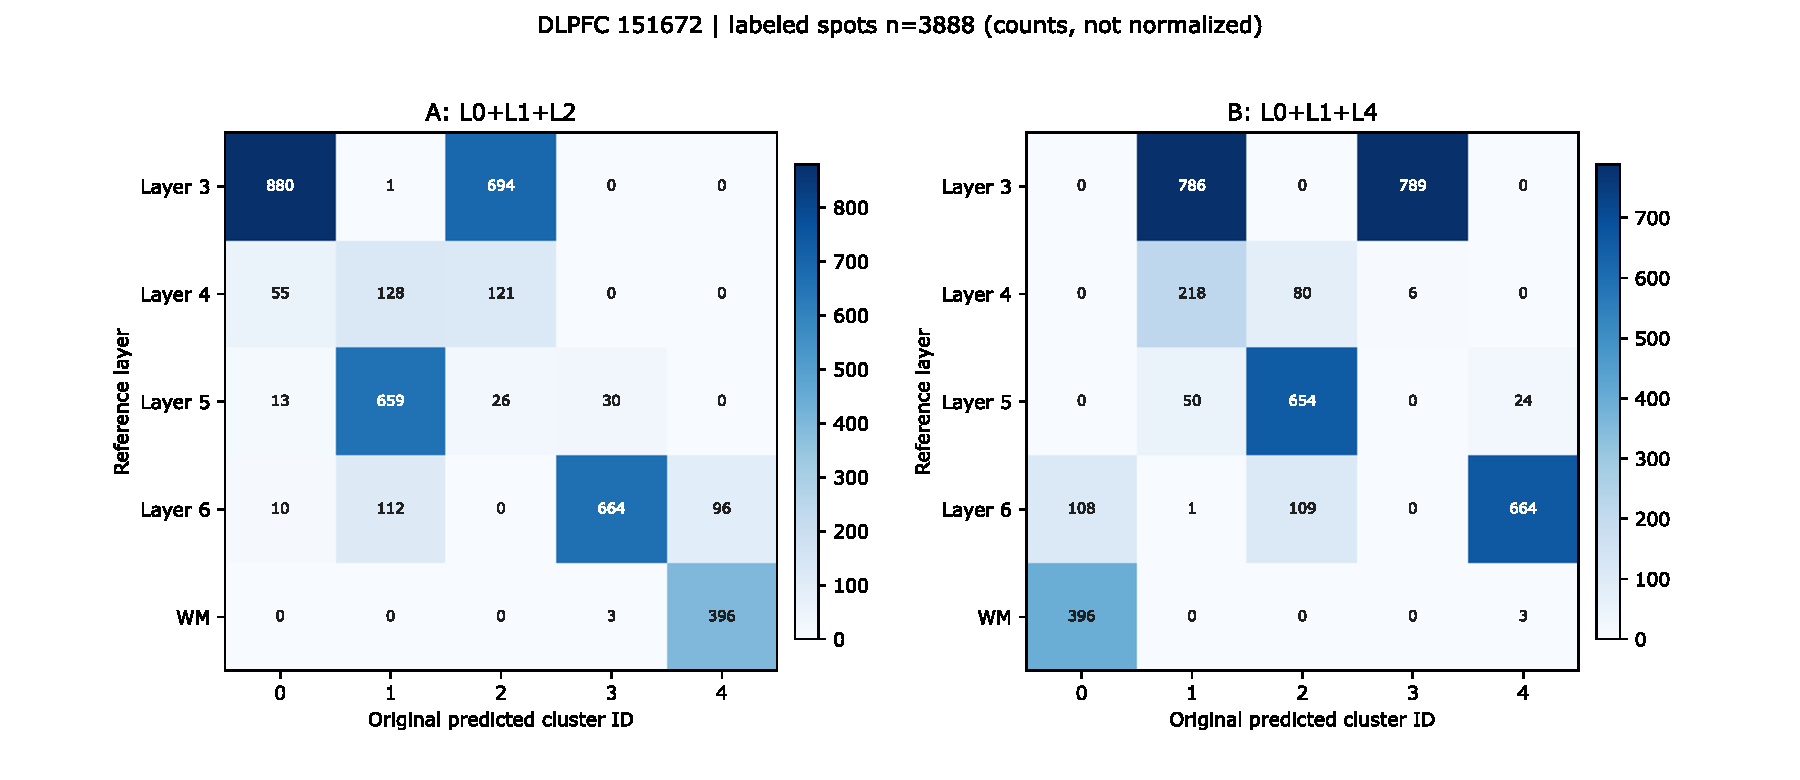
\includegraphics[width=0.97\linewidth,height=0.72\textheight,keepaspectratio]{E4_SOURCE_FIGURES_20261122_RELEASE/figures_pdf/151672/151672_reference_A_B_confusion.pdf}
\captionof{figure}{DLPFC切片151672：参考层与A/B簇交叉计数图（原始E4图件转换的矢量PDF；聚类编号未根据参考标签重排）。}
\label{fig:cc-e4-app-151672-confusion}
\end{minipage}\par\medskip
}{%
\par\noindent\emph{[待插入原始E4图件：151672_reference_A_B_confusion.svg]}\par
}
\subsection{DLPFC切片151673}
\IfFileExists{E4_SOURCE_FIGURES_20261122_RELEASE/figures_pdf/151673/151673_reference_A_B_spatial.pdf}{%
\par\noindent\begin{minipage}{\linewidth}
\centering
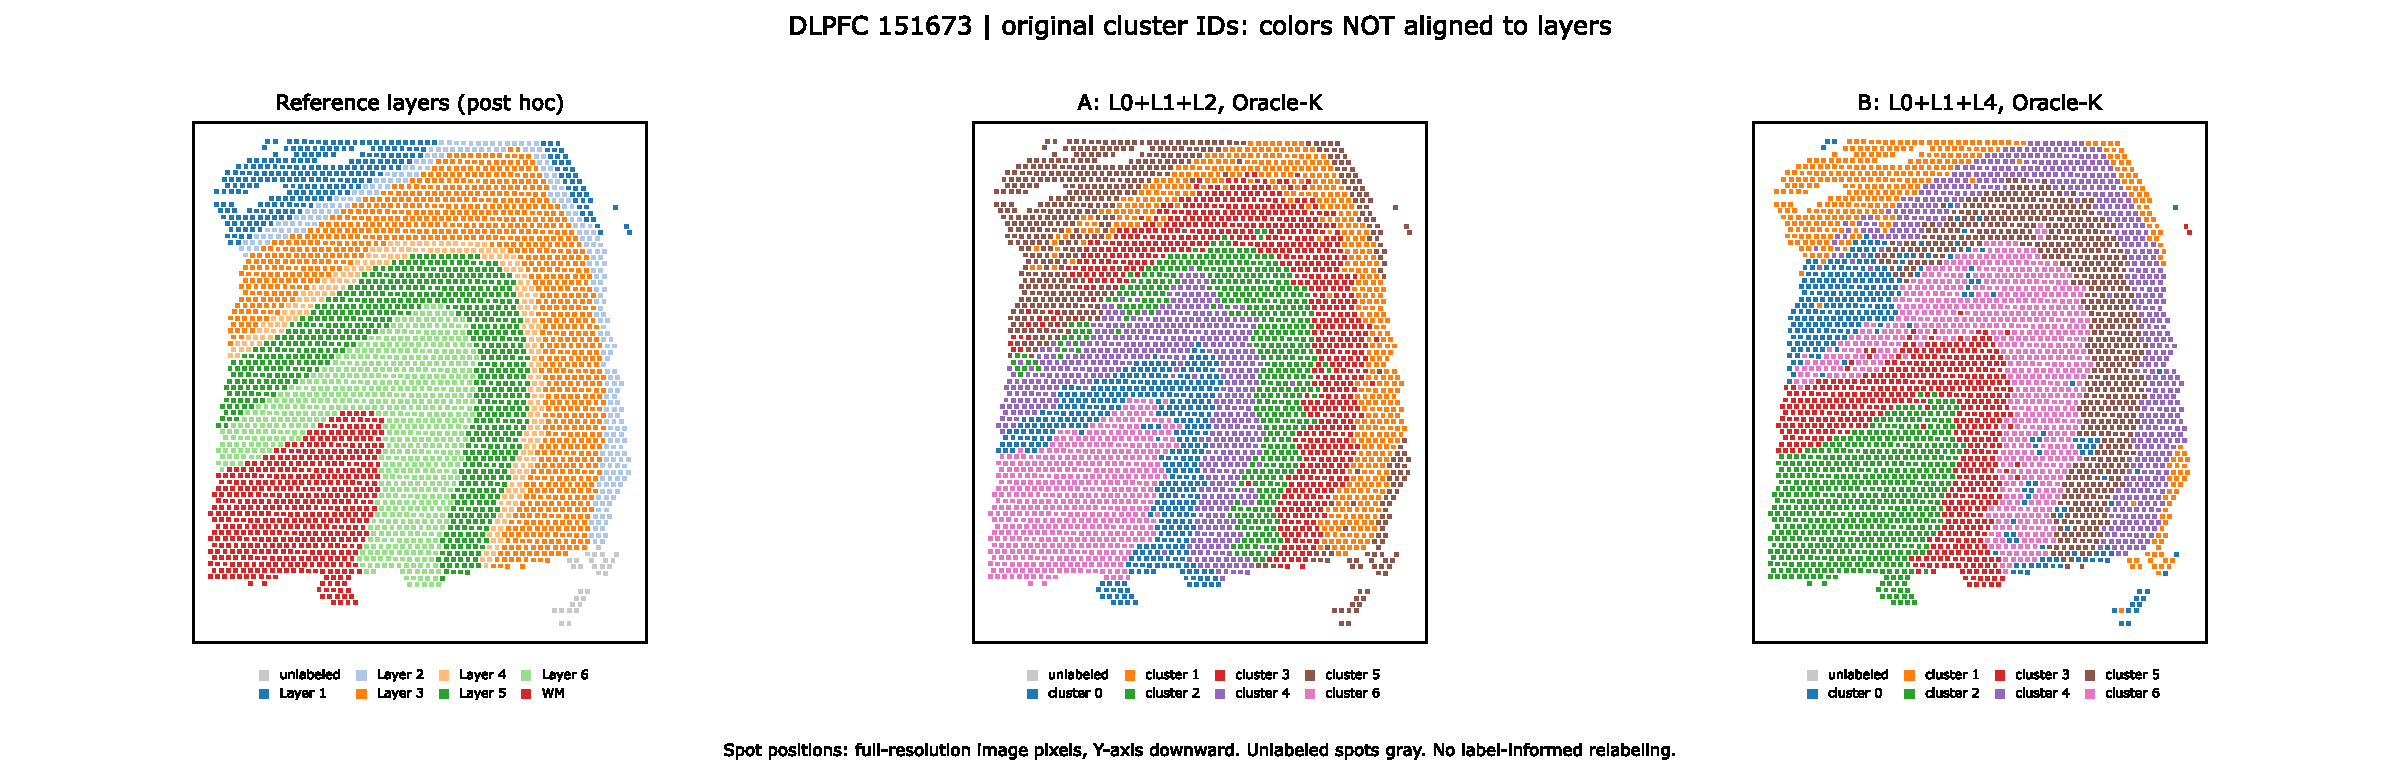
\includegraphics[width=0.97\linewidth,height=0.72\textheight,keepaspectratio]{E4_SOURCE_FIGURES_20261122_RELEASE/figures_pdf/151673/151673_reference_A_B_spatial.pdf}
\captionof{figure}{DLPFC切片151673：参考层与A/B原始聚类三联图（原始E4图件转换的矢量PDF；聚类编号未根据参考标签重排）。}
\label{fig:cc-e4-app-151673-map}
\end{minipage}\par\medskip
}{%
\par\noindent\emph{[待插入原始E4图件：151673_reference_A_B_spatial.svg]}\par
}
\IfFileExists{E4_SOURCE_FIGURES_20261122_RELEASE/figures_pdf/151673/151673_MOBP_PCP4_SNAP25_expression.pdf}{%
\par\noindent\begin{minipage}{\linewidth}
\centering
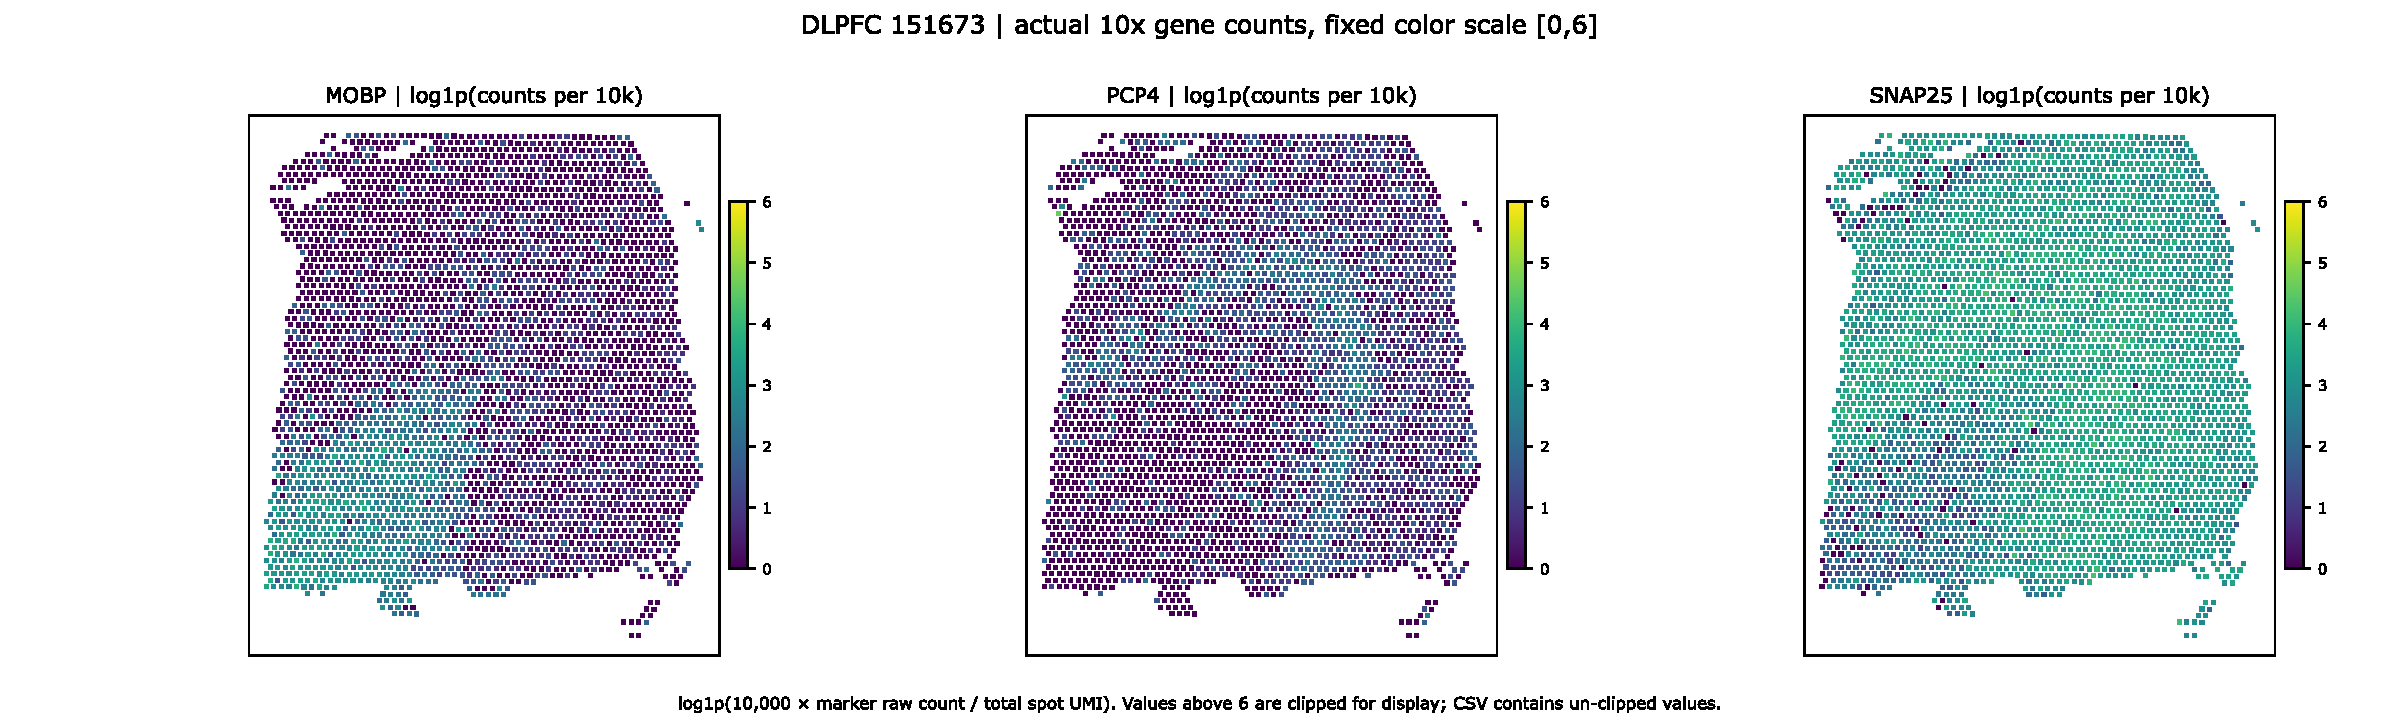
\includegraphics[width=0.97\linewidth,height=0.72\textheight,keepaspectratio]{E4_SOURCE_FIGURES_20261122_RELEASE/figures_pdf/151673/151673_MOBP_PCP4_SNAP25_expression.pdf}
\captionof{figure}{DLPFC切片151673：MOBP/PCP4/SNAP25表达三联图（原始E4图件转换的矢量PDF；聚类编号未根据参考标签重排）。}
\label{fig:cc-e4-app-151673-markers}
\end{minipage}\par\medskip
}{%
\par\noindent\emph{[待插入原始E4图件：151673_MOBP_PCP4_SNAP25_expression.svg]}\par
}
\IfFileExists{E4_SOURCE_FIGURES_20261122_RELEASE/figures_pdf/151673/151673_reference_A_B_confusion.pdf}{%
\par\noindent\begin{minipage}{\linewidth}
\centering
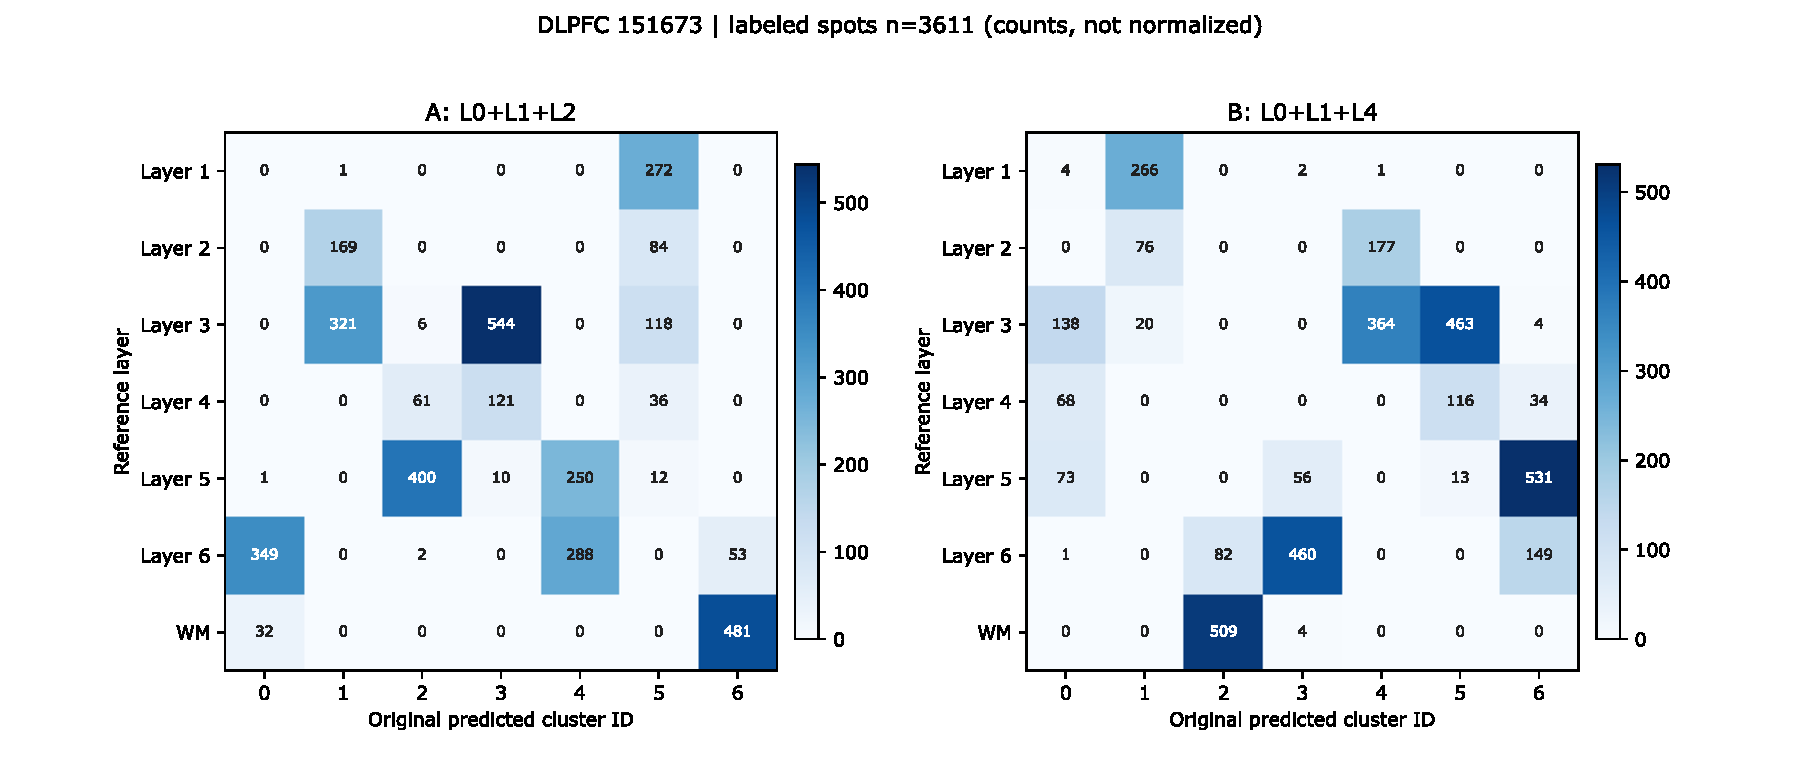
\includegraphics[width=0.97\linewidth,height=0.72\textheight,keepaspectratio]{E4_SOURCE_FIGURES_20261122_RELEASE/figures_pdf/151673/151673_reference_A_B_confusion.pdf}
\captionof{figure}{DLPFC切片151673：参考层与A/B簇交叉计数图（原始E4图件转换的矢量PDF；聚类编号未根据参考标签重排）。}
\label{fig:cc-e4-app-151673-confusion}
\end{minipage}\par\medskip
}{%
\par\noindent\emph{[待插入原始E4图件：151673_reference_A_B_confusion.svg]}\par
}
\subsection{DLPFC切片151674}
\IfFileExists{E4_SOURCE_FIGURES_20261122_RELEASE/figures_pdf/151674/151674_reference_A_B_spatial.pdf}{%
\par\noindent\begin{minipage}{\linewidth}
\centering
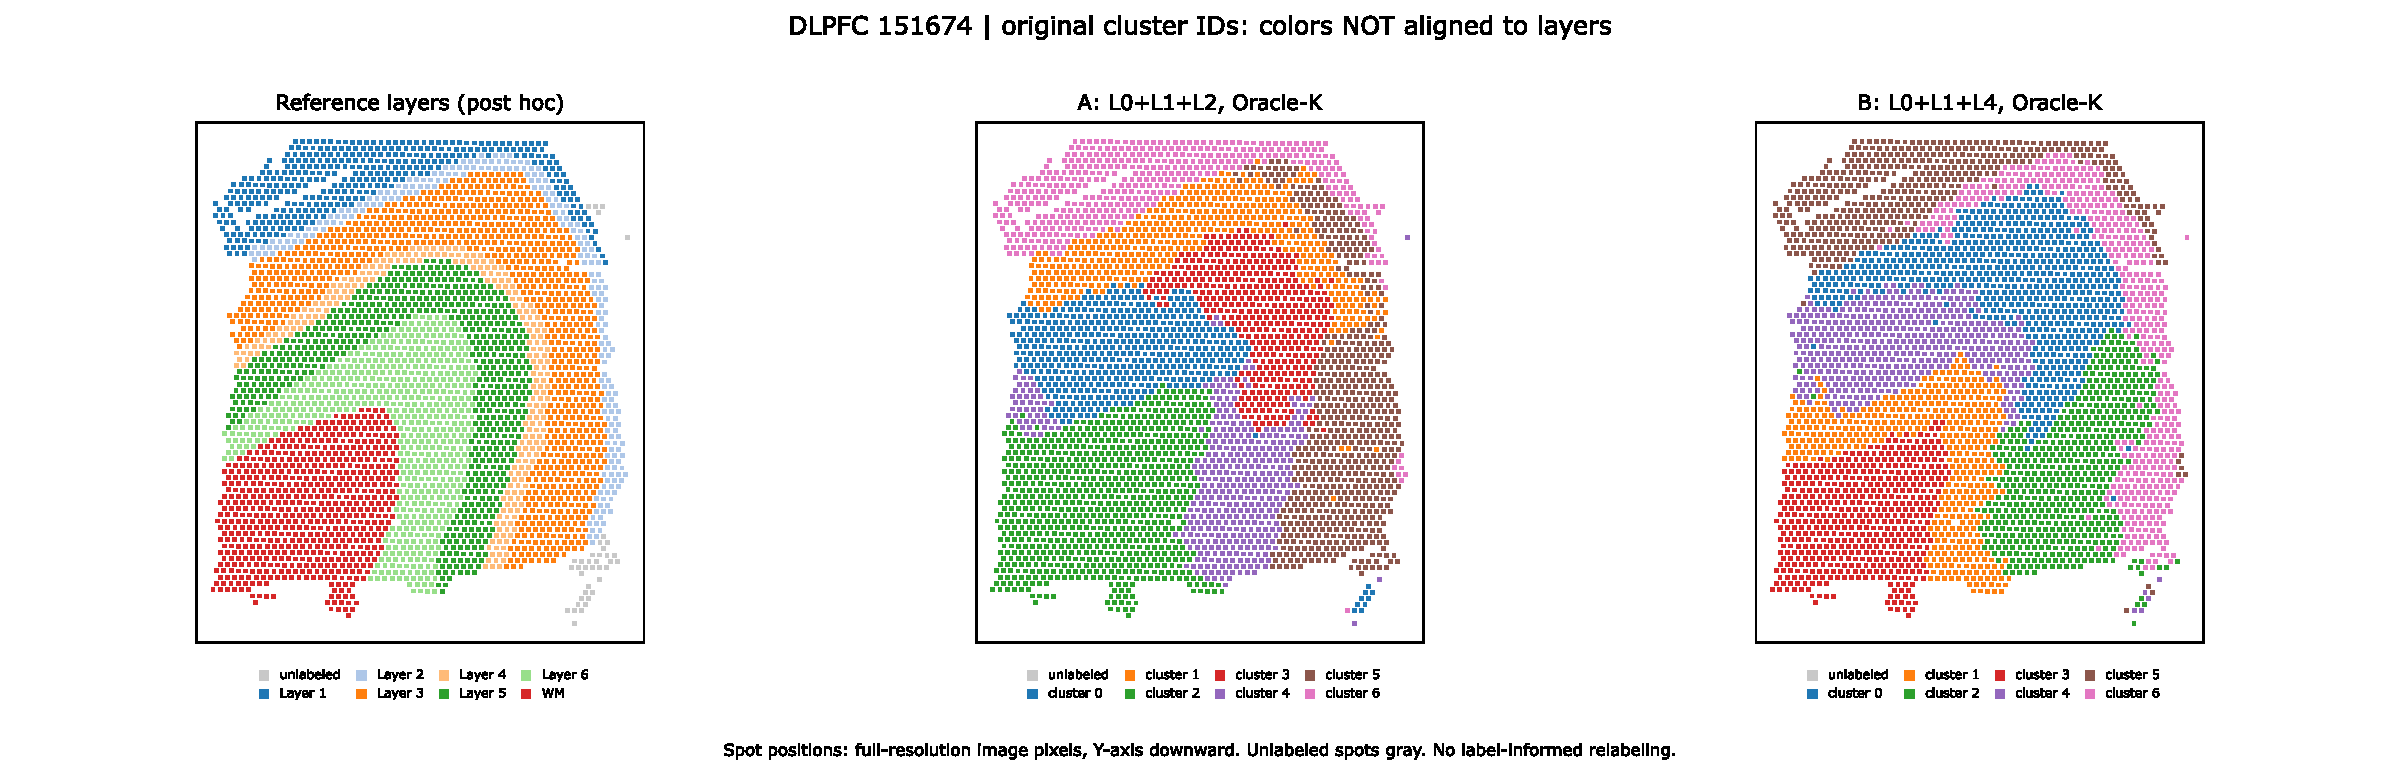
\includegraphics[width=0.97\linewidth,height=0.72\textheight,keepaspectratio]{E4_SOURCE_FIGURES_20261122_RELEASE/figures_pdf/151674/151674_reference_A_B_spatial.pdf}
\captionof{figure}{DLPFC切片151674：参考层与A/B原始聚类三联图（原始E4图件转换的矢量PDF；聚类编号未根据参考标签重排）。}
\label{fig:cc-e4-app-151674-map}
\end{minipage}\par\medskip
}{%
\par\noindent\emph{[待插入原始E4图件：151674_reference_A_B_spatial.svg]}\par
}
\IfFileExists{E4_SOURCE_FIGURES_20261122_RELEASE/figures_pdf/151674/151674_MOBP_PCP4_SNAP25_expression.pdf}{%
\par\noindent\begin{minipage}{\linewidth}
\centering
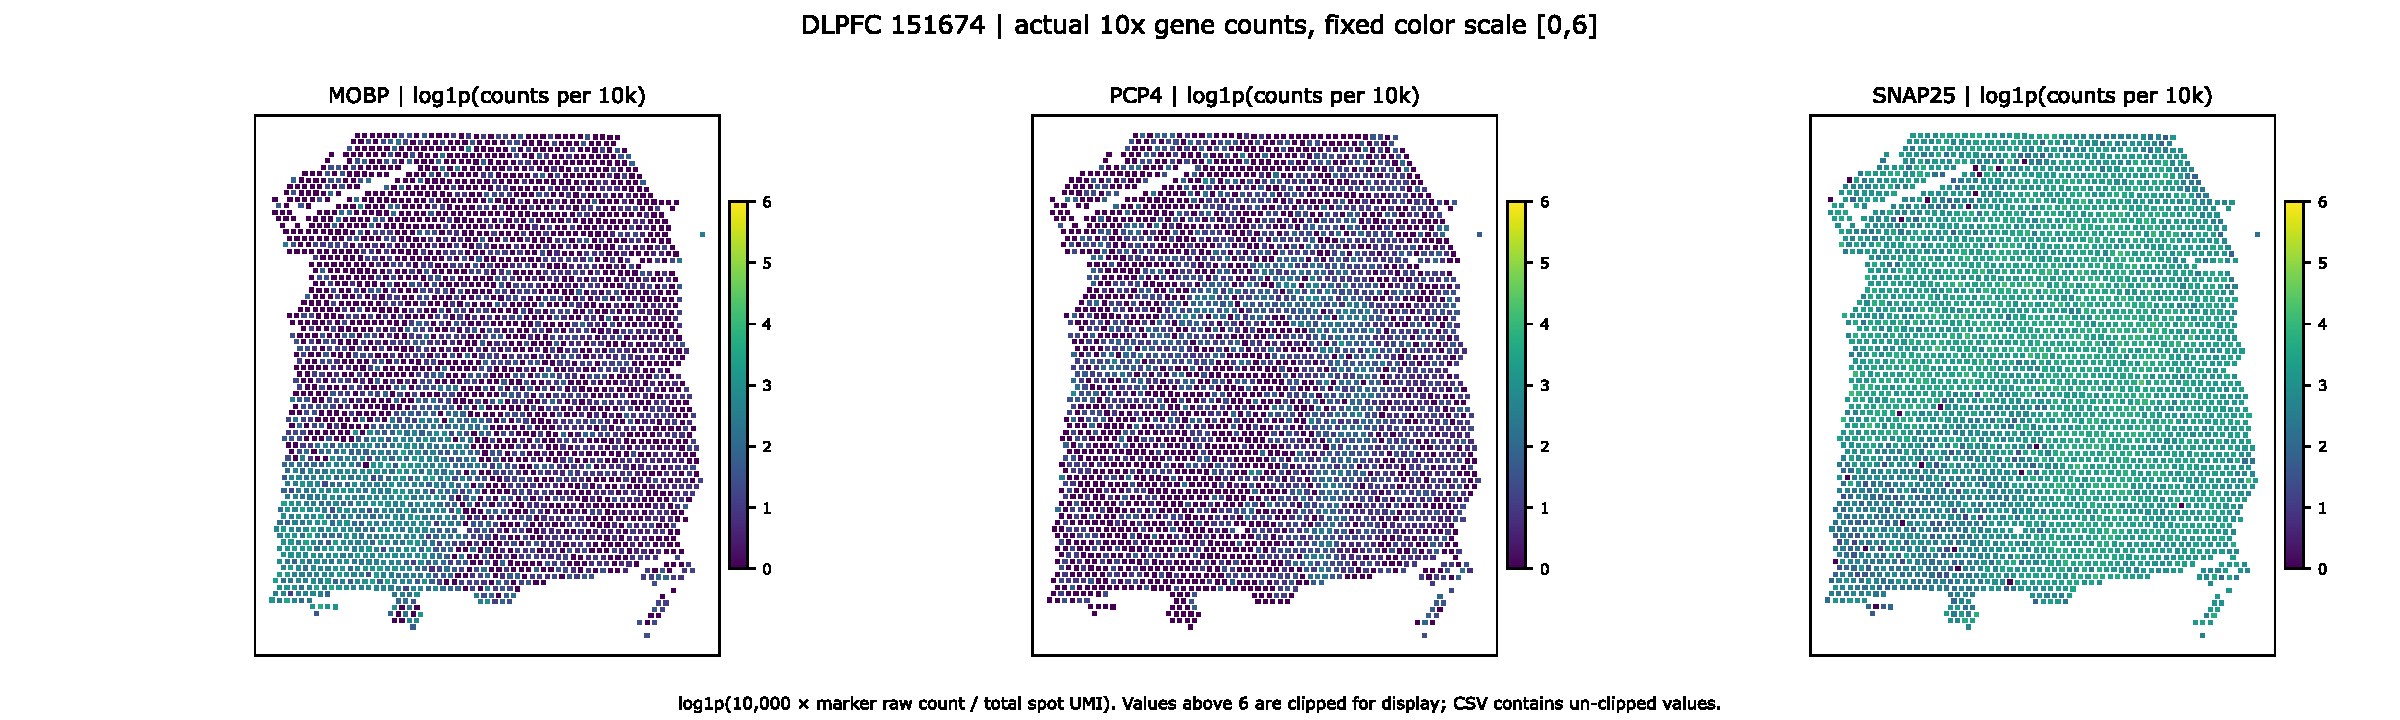
\includegraphics[width=0.97\linewidth,height=0.72\textheight,keepaspectratio]{E4_SOURCE_FIGURES_20261122_RELEASE/figures_pdf/151674/151674_MOBP_PCP4_SNAP25_expression.pdf}
\captionof{figure}{DLPFC切片151674：MOBP/PCP4/SNAP25表达三联图（原始E4图件转换的矢量PDF；聚类编号未根据参考标签重排）。}
\label{fig:cc-e4-app-151674-markers}
\end{minipage}\par\medskip
}{%
\par\noindent\emph{[待插入原始E4图件：151674_MOBP_PCP4_SNAP25_expression.svg]}\par
}
\IfFileExists{E4_SOURCE_FIGURES_20261122_RELEASE/figures_pdf/151674/151674_reference_A_B_confusion.pdf}{%
\par\noindent\begin{minipage}{\linewidth}
\centering
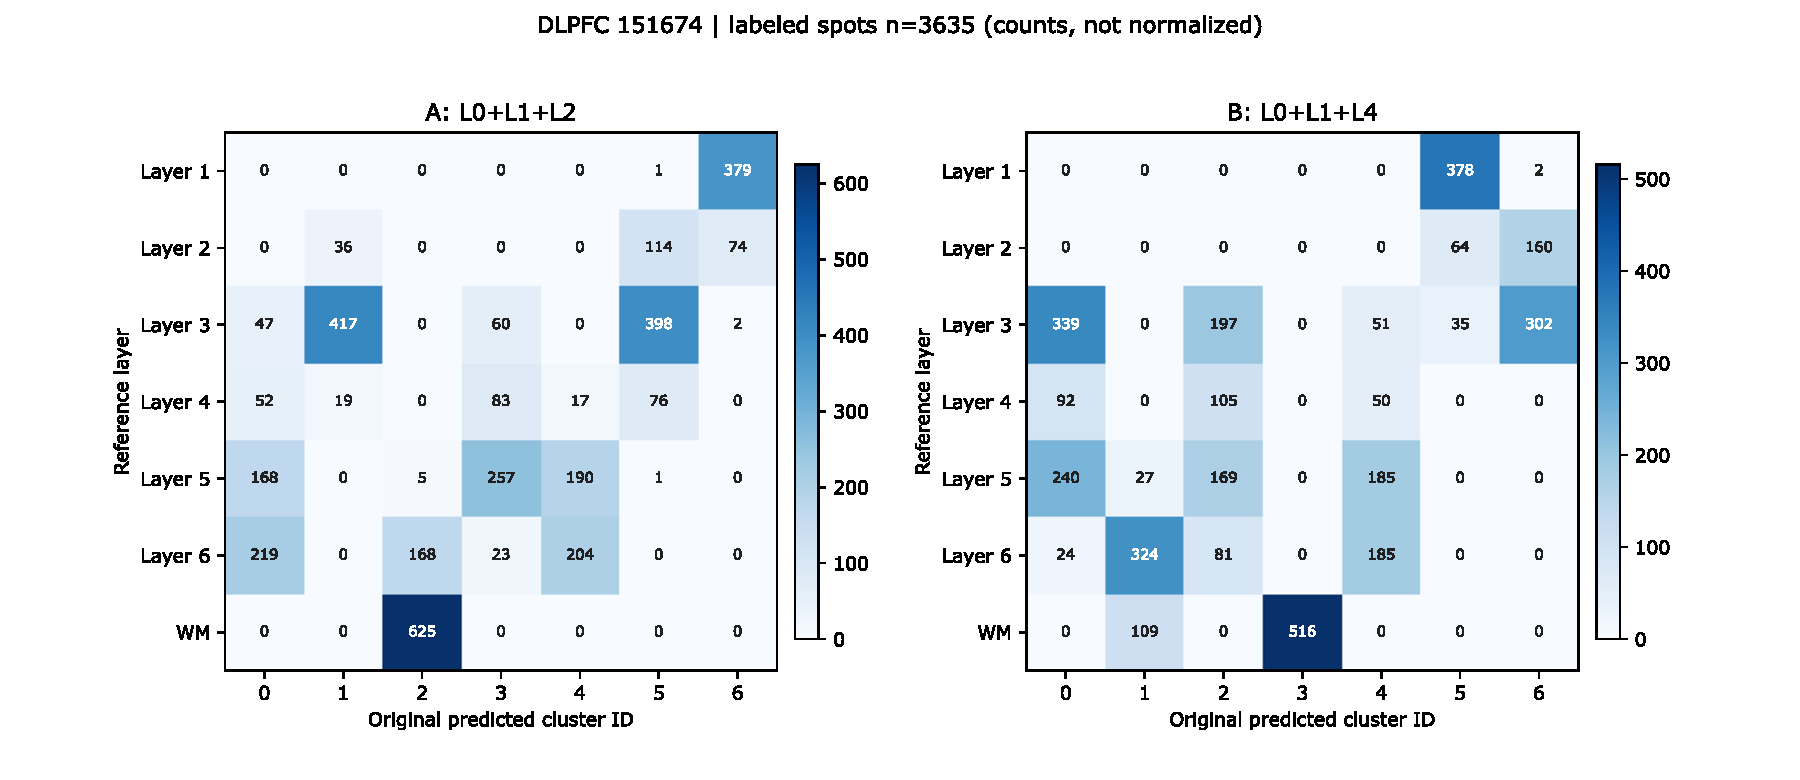
\includegraphics[width=0.97\linewidth,height=0.72\textheight,keepaspectratio]{E4_SOURCE_FIGURES_20261122_RELEASE/figures_pdf/151674/151674_reference_A_B_confusion.pdf}
\captionof{figure}{DLPFC切片151674：参考层与A/B簇交叉计数图（原始E4图件转换的矢量PDF；聚类编号未根据参考标签重排）。}
\label{fig:cc-e4-app-151674-confusion}
\end{minipage}\par\medskip
}{%
\par\noindent\emph{[待插入原始E4图件：151674_reference_A_B_confusion.svg]}\par
}
\subsection{DLPFC切片151675}
\IfFileExists{E4_SOURCE_FIGURES_20261122_RELEASE/figures_pdf/151675/151675_reference_A_B_spatial.pdf}{%
\par\noindent\begin{minipage}{\linewidth}
\centering
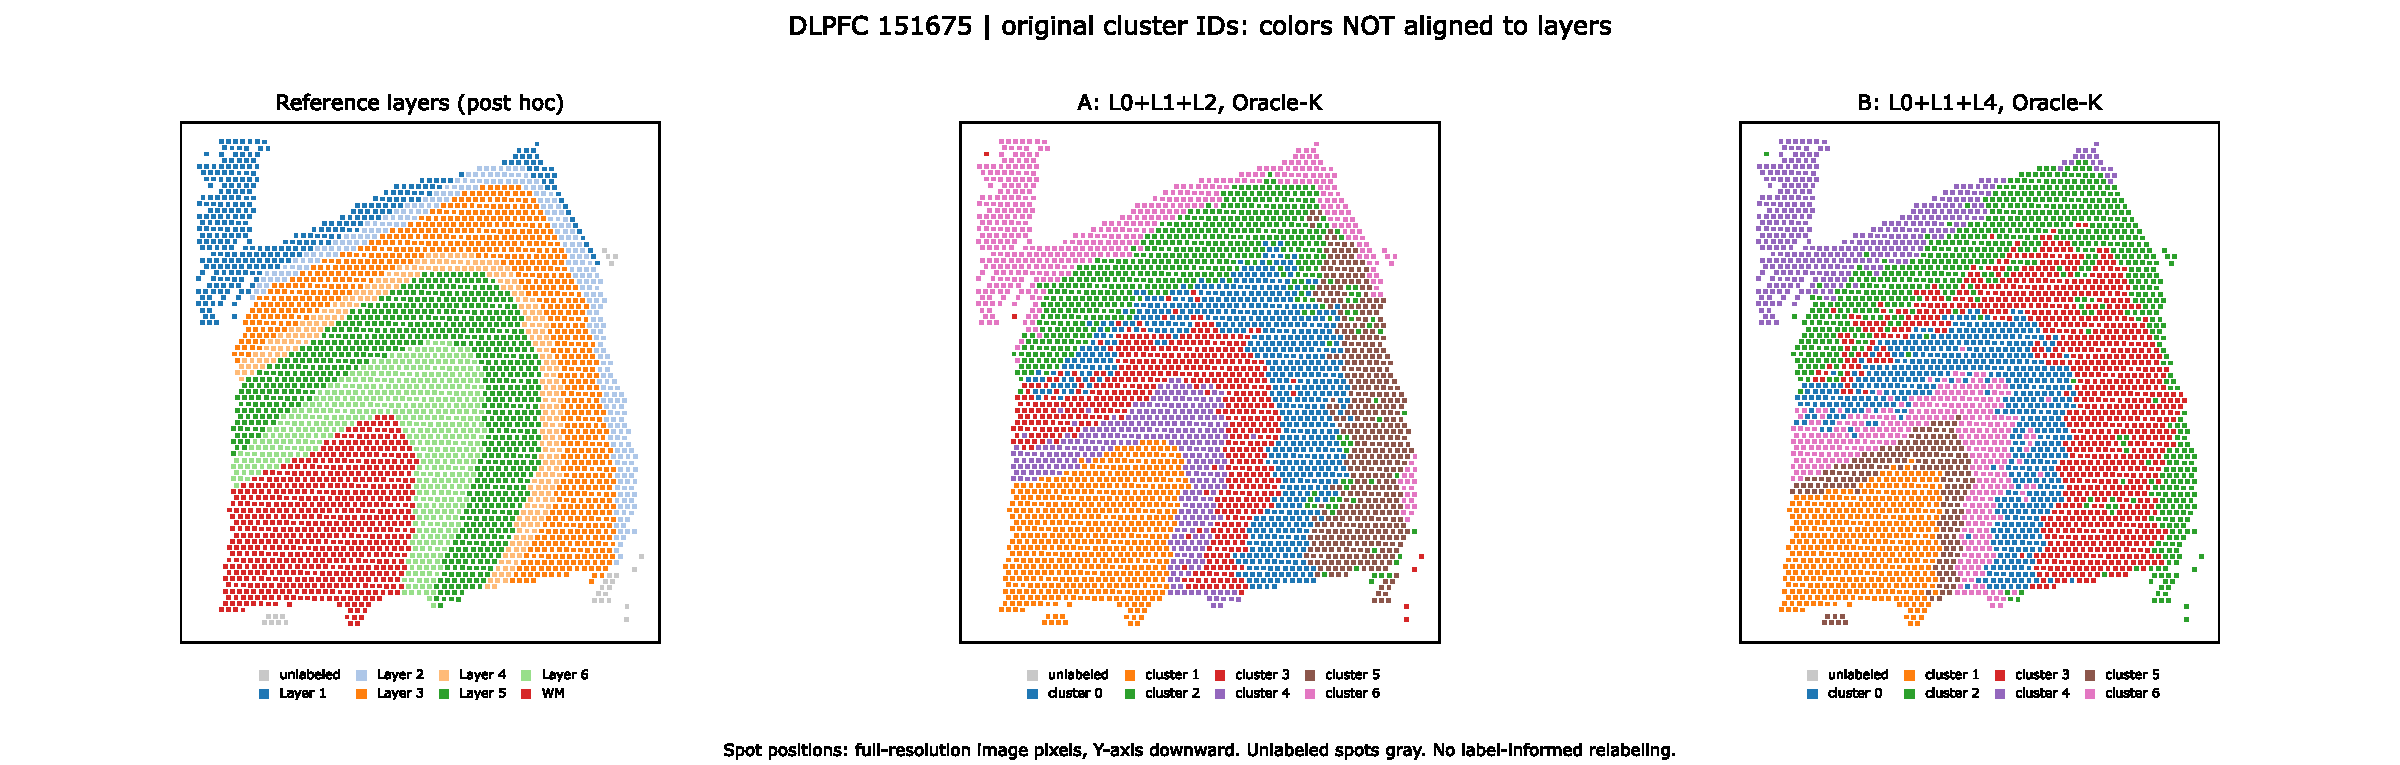
\includegraphics[width=0.97\linewidth,height=0.72\textheight,keepaspectratio]{E4_SOURCE_FIGURES_20261122_RELEASE/figures_pdf/151675/151675_reference_A_B_spatial.pdf}
\captionof{figure}{DLPFC切片151675：参考层与A/B原始聚类三联图（原始E4图件转换的矢量PDF；聚类编号未根据参考标签重排）。}
\label{fig:cc-e4-app-151675-map}
\end{minipage}\par\medskip
}{%
\par\noindent\emph{[待插入原始E4图件：151675_reference_A_B_spatial.svg]}\par
}
\IfFileExists{E4_SOURCE_FIGURES_20261122_RELEASE/figures_pdf/151675/151675_MOBP_PCP4_SNAP25_expression.pdf}{%
\par\noindent\begin{minipage}{\linewidth}
\centering
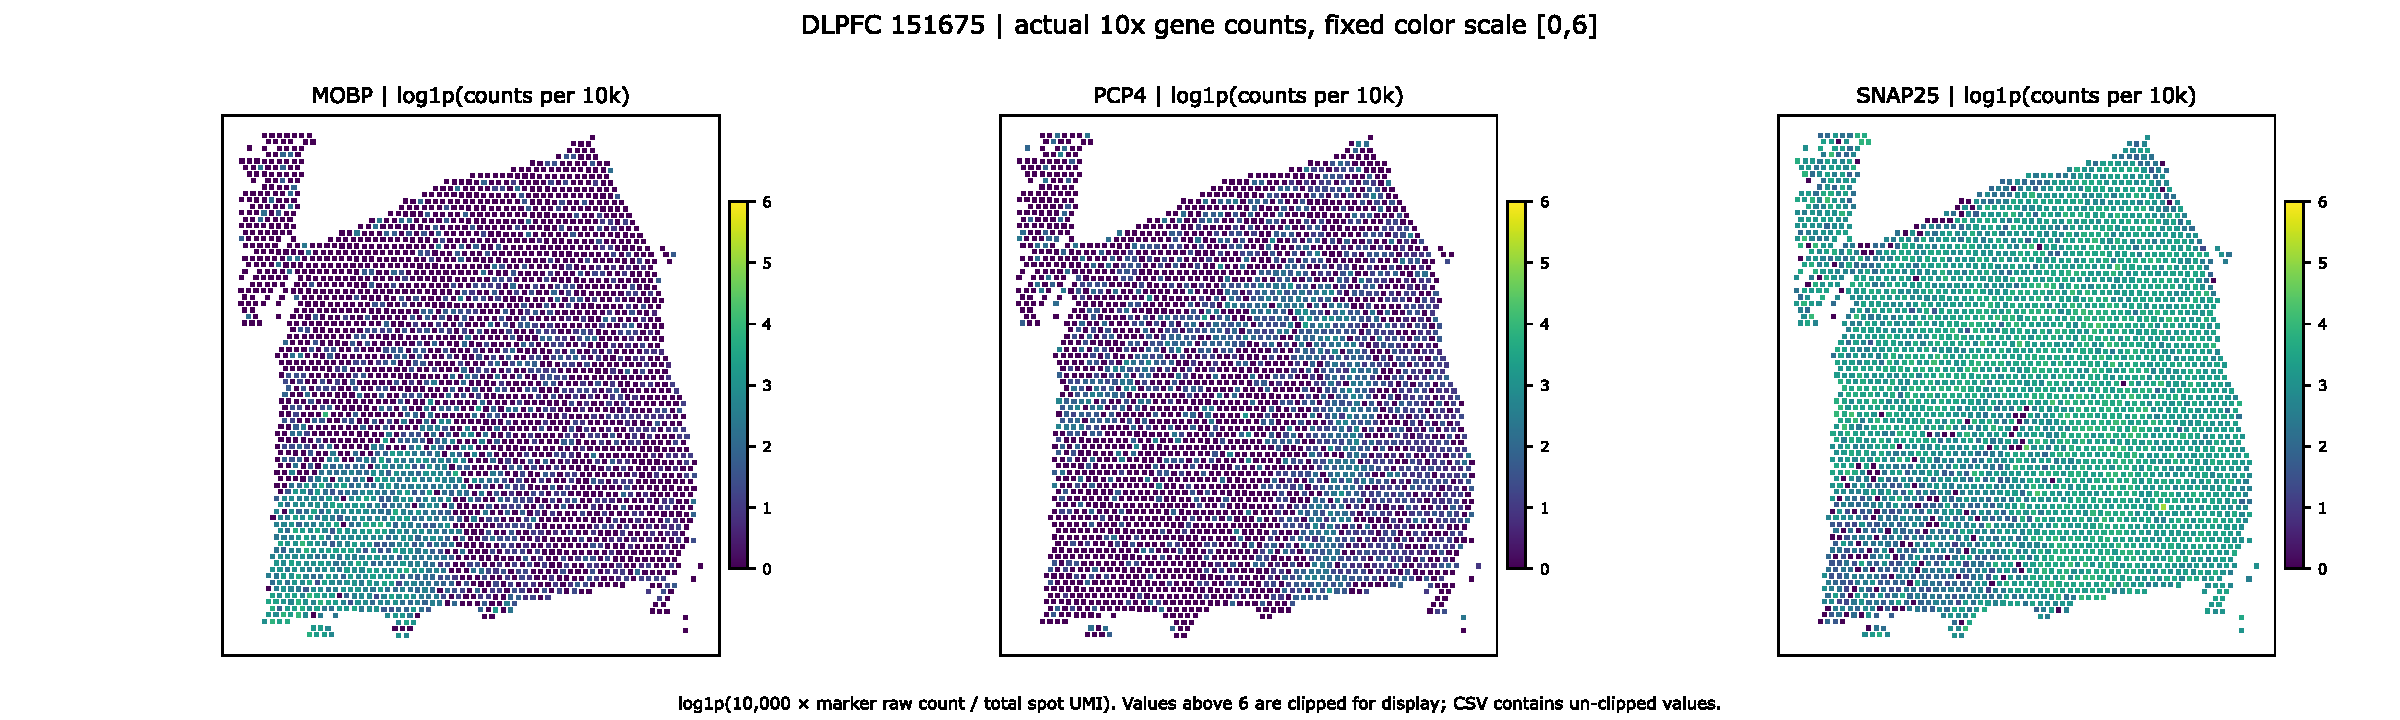
\includegraphics[width=0.97\linewidth,height=0.72\textheight,keepaspectratio]{E4_SOURCE_FIGURES_20261122_RELEASE/figures_pdf/151675/151675_MOBP_PCP4_SNAP25_expression.pdf}
\captionof{figure}{DLPFC切片151675：MOBP/PCP4/SNAP25表达三联图（原始E4图件转换的矢量PDF；聚类编号未根据参考标签重排）。}
\label{fig:cc-e4-app-151675-markers}
\end{minipage}\par\medskip
}{%
\par\noindent\emph{[待插入原始E4图件：151675_MOBP_PCP4_SNAP25_expression.svg]}\par
}
\IfFileExists{E4_SOURCE_FIGURES_20261122_RELEASE/figures_pdf/151675/151675_reference_A_B_confusion.pdf}{%
\par\noindent\begin{minipage}{\linewidth}
\centering
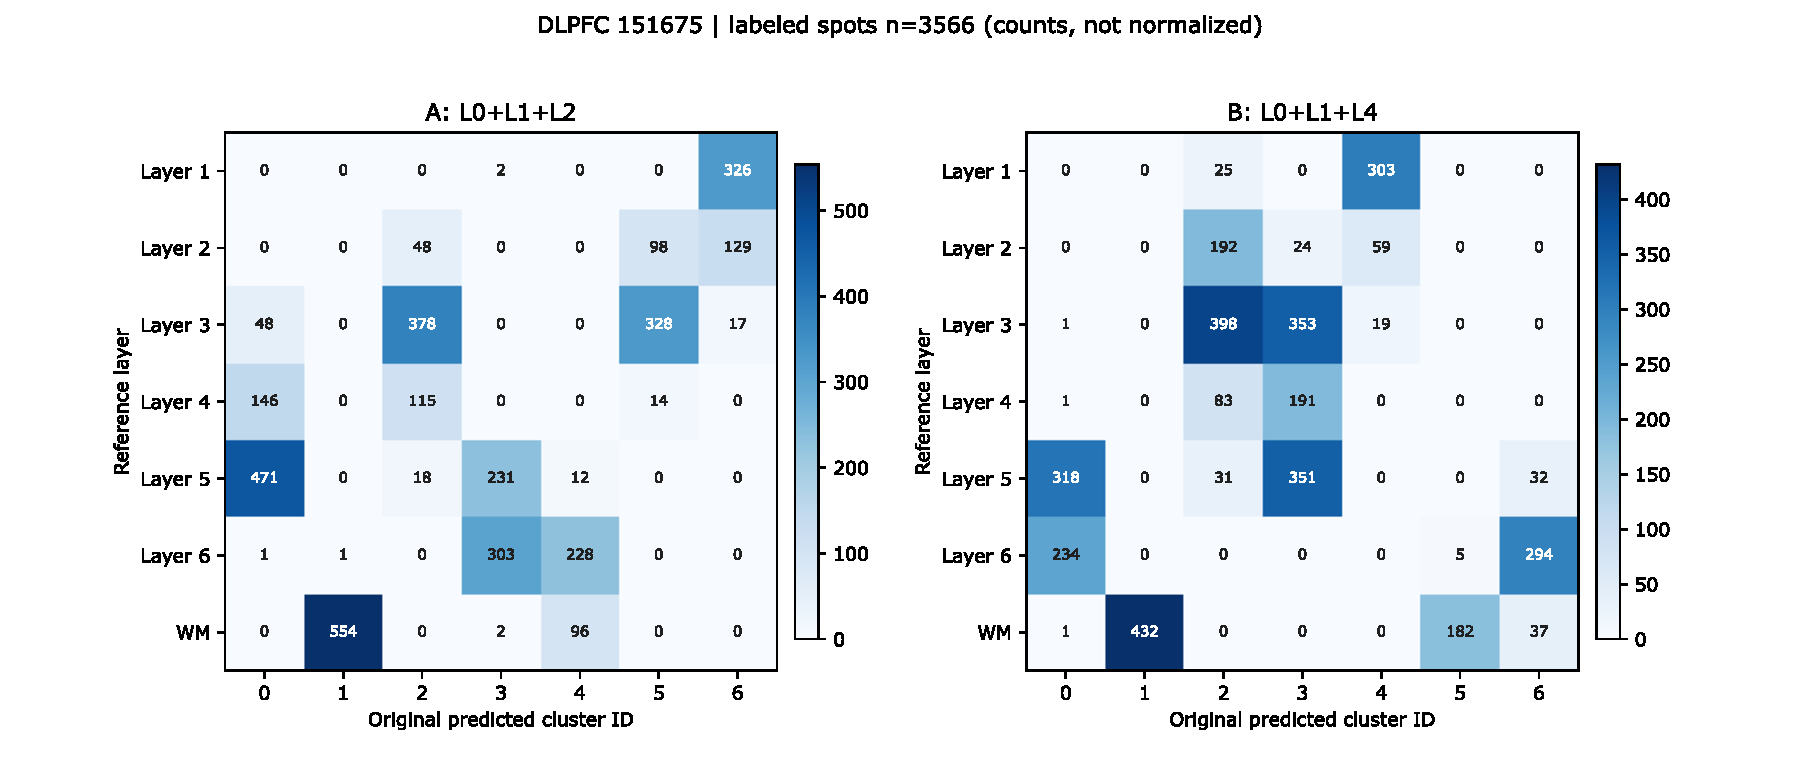
\includegraphics[width=0.97\linewidth,height=0.72\textheight,keepaspectratio]{E4_SOURCE_FIGURES_20261122_RELEASE/figures_pdf/151675/151675_reference_A_B_confusion.pdf}
\captionof{figure}{DLPFC切片151675：参考层与A/B簇交叉计数图（原始E4图件转换的矢量PDF；聚类编号未根据参考标签重排）。}
\label{fig:cc-e4-app-151675-confusion}
\end{minipage}\par\medskip
}{%
\par\noindent\emph{[待插入原始E4图件：151675_reference_A_B_confusion.svg]}\par
}
\subsection{DLPFC切片151676}
\IfFileExists{E4_SOURCE_FIGURES_20261122_RELEASE/figures_pdf/151676/151676_reference_A_B_spatial.pdf}{%
\par\noindent\begin{minipage}{\linewidth}
\centering
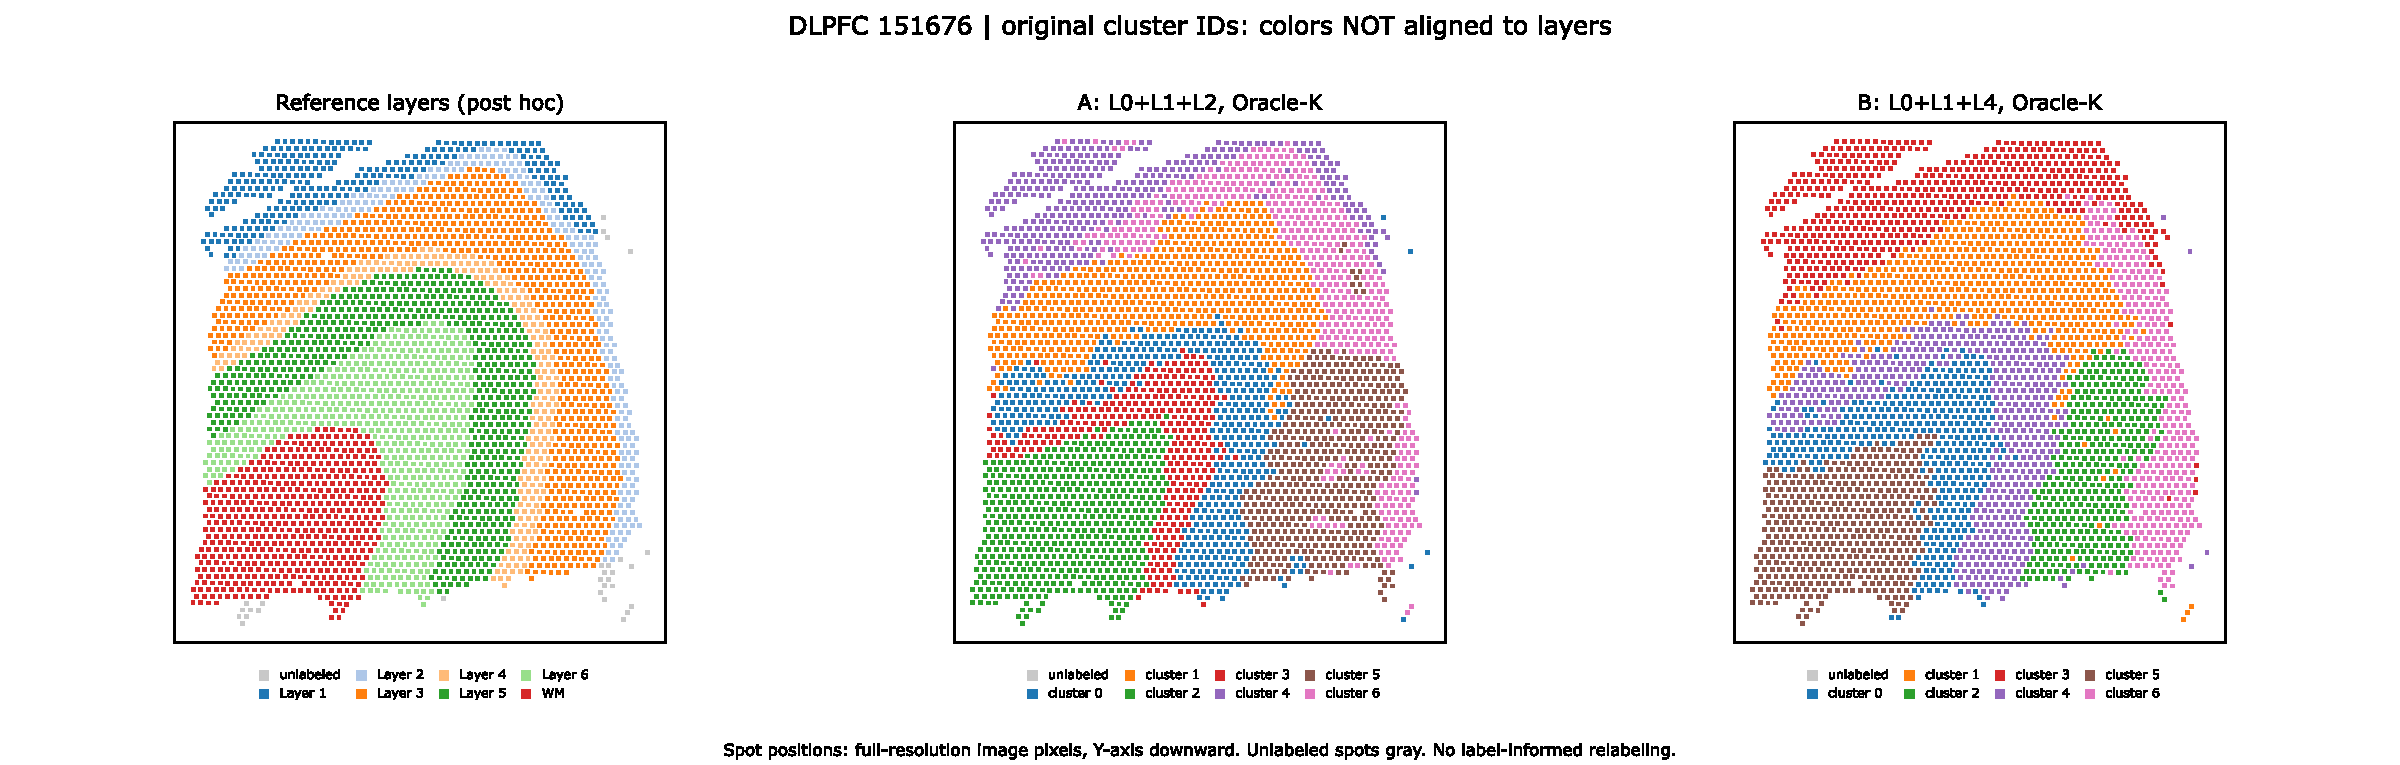
\includegraphics[width=0.97\linewidth,height=0.72\textheight,keepaspectratio]{E4_SOURCE_FIGURES_20261122_RELEASE/figures_pdf/151676/151676_reference_A_B_spatial.pdf}
\captionof{figure}{DLPFC切片151676：参考层与A/B原始聚类三联图（原始E4图件转换的矢量PDF；聚类编号未根据参考标签重排）。}
\label{fig:cc-e4-app-151676-map}
\end{minipage}\par\medskip
}{%
\par\noindent\emph{[待插入原始E4图件：151676_reference_A_B_spatial.svg]}\par
}
\IfFileExists{E4_SOURCE_FIGURES_20261122_RELEASE/figures_pdf/151676/151676_MOBP_PCP4_SNAP25_expression.pdf}{%
\par\noindent\begin{minipage}{\linewidth}
\centering
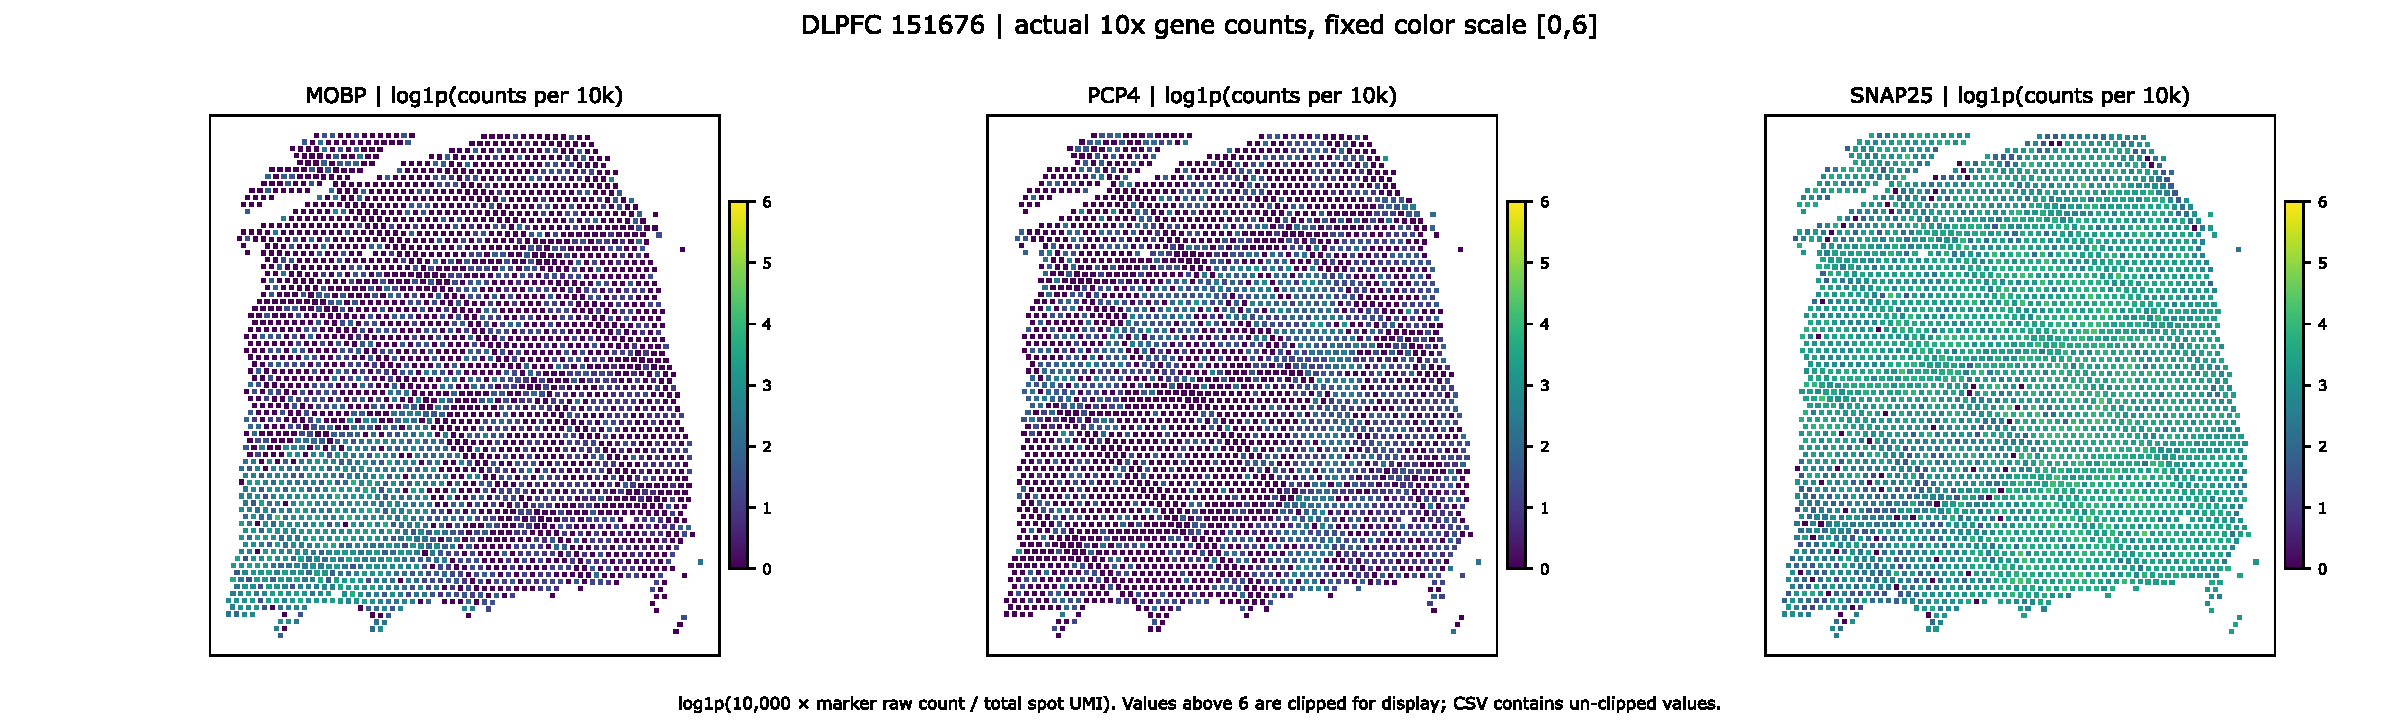
\includegraphics[width=0.97\linewidth,height=0.72\textheight,keepaspectratio]{E4_SOURCE_FIGURES_20261122_RELEASE/figures_pdf/151676/151676_MOBP_PCP4_SNAP25_expression.pdf}
\captionof{figure}{DLPFC切片151676：MOBP/PCP4/SNAP25表达三联图（原始E4图件转换的矢量PDF；聚类编号未根据参考标签重排）。}
\label{fig:cc-e4-app-151676-markers}
\end{minipage}\par\medskip
}{%
\par\noindent\emph{[待插入原始E4图件：151676_MOBP_PCP4_SNAP25_expression.svg]}\par
}
\IfFileExists{E4_SOURCE_FIGURES_20261122_RELEASE/figures_pdf/151676/151676_reference_A_B_confusion.pdf}{%
\par\noindent\begin{minipage}{\linewidth}
\centering
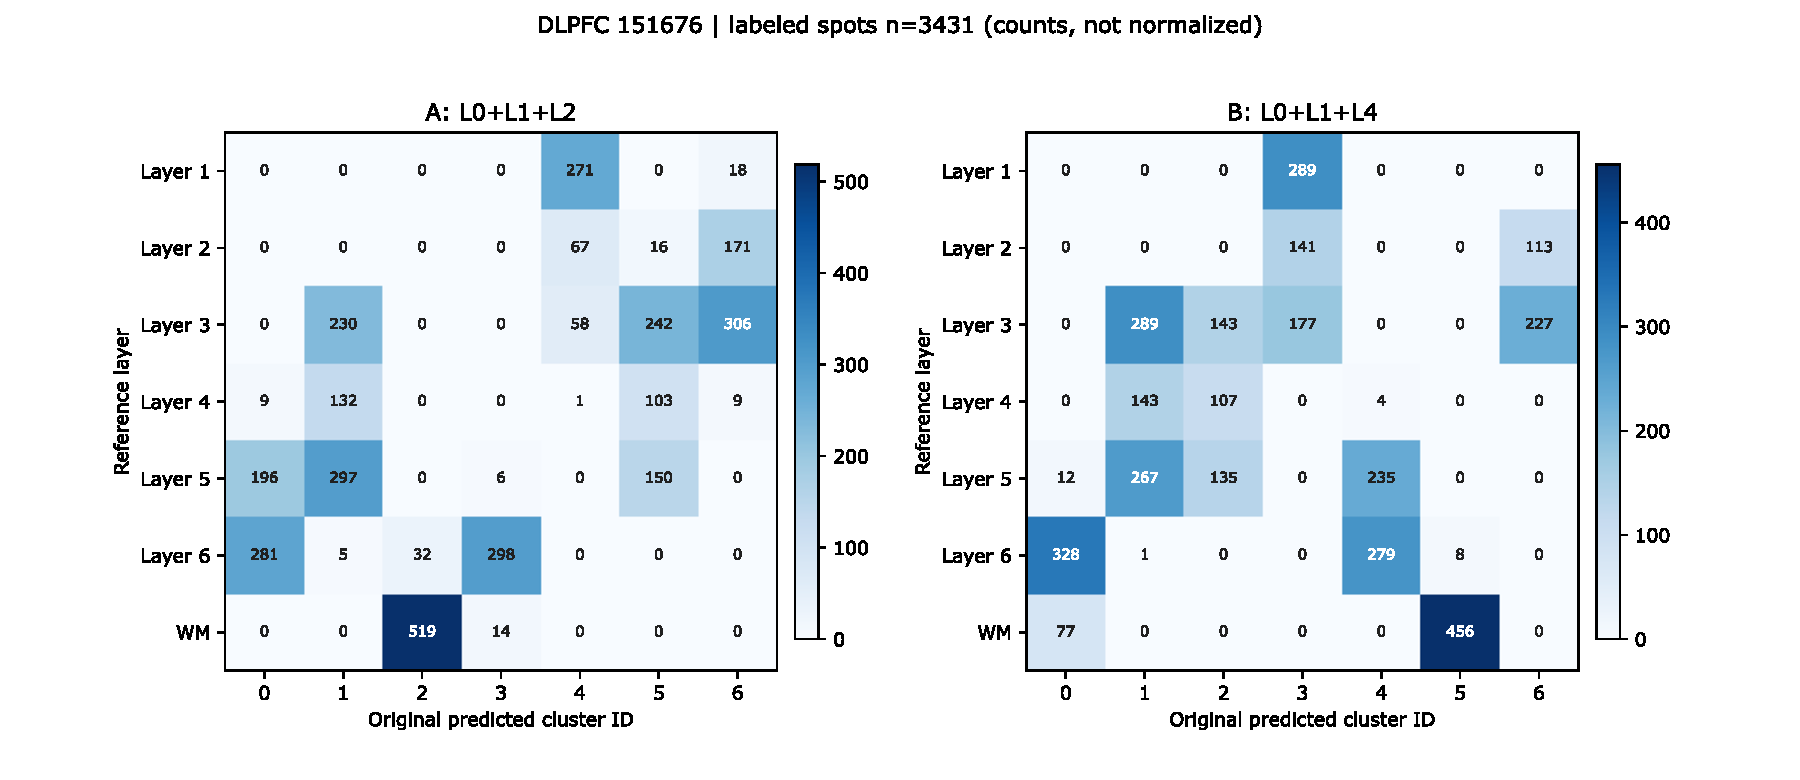
\includegraphics[width=0.97\linewidth,height=0.72\textheight,keepaspectratio]{E4_SOURCE_FIGURES_20261122_RELEASE/figures_pdf/151676/151676_reference_A_B_confusion.pdf}
\captionof{figure}{DLPFC切片151676：参考层与A/B簇交叉计数图（原始E4图件转换的矢量PDF；聚类编号未根据参考标签重排）。}
\label{fig:cc-e4-app-151676-confusion}
\end{minipage}\par\medskip
}{%
\par\noindent\emph{[待插入原始E4图件：151676_reference_A_B_confusion.svg]}\par
}

}{}

\bibliographystyle{unsrt}
\bibliography{thesis_cellcharter_references_rev_p0_20261124}
\end{document}
